\documentclass[11pt,a4paper,oneside]{report}
\usepackage[T1]{fontenc}
\usepackage[utf8]{inputenc}
\usepackage[english]{babel}
\babelprovide[import,main]{french}
\usepackage{lmodern}
\usepackage{amsmath,amssymb,amsthm}
\usepackage{graphicx}
\usepackage{booktabs,longtable,tabularx,array}
\usepackage[a4paper,margin=2.5cm]{geometry}
\usepackage{microtype}
\usepackage{xcolor}
\usepackage{listings}
\usepackage{caption}
\usepackage{hyperref}
\definecolor{academicblue}{RGB}{29,63,91}
\hypersetup{colorlinks=true,linkcolor=academicblue,citecolor=academicblue,
 urlcolor=academicblue,pdftitle={Traitement d'images par des équations aux dérivées partielles},
 pdfauthor={Mhamed Halhoul et Khalil Amraoui},
 pdfsubject={Projet scientifique de Master : Modélisation déterministe et applications},bookmarksdepth=2}
\author{Mhamed Halhoul et Khalil Amraoui}
\graphicspath{{../results/extended/figures/}}
\captionsetup{font=small,labelfont=bf}
\setlength{\parindent}{1.3em}
\setlength{\parskip}{0.25em}
\setlength{\emergencystretch}{2em}
\setcounter{tocdepth}{1}
\newcommand{\dd}{\mathrm{d}}
\newcommand{\R}{\mathbb{R}}
\newcommand{\norm}[1]{\left\lVert#1\right\rVert}
\newcommand{\utrue}{u_{\mathrm{true}}}
\newcommand{\dt}{\Delta t}
\newcommand{\dx}{\Delta x}
\newcommand{\dy}{\Delta y}
\lstset{columns=fullflexible,keepspaces=true,showstringspaces=false,
 breaklines=true,basicstyle=\ttfamily\small}

\begin{document}
\selectlanguage{french}
\hypersetup{pageanchor=false}
\begin{titlepage}
\thispagestyle{empty}
\definecolor{coverink}{RGB}{20,39,62}
\definecolor{coverteal}{RGB}{0,125,133}
\begin{minipage}[c]{0.67\linewidth}

\includegraphics[width=6.2cm]{../assets/logos/uae.png}
\end{minipage}\hfill
\begin{minipage}[c]{0.20\linewidth}
\raggedleft
\includegraphics[height=2.0cm]{../assets/logos/fpl.png}
\end{minipage}
\vspace{0.55cm}
\begin{center}
{\Large\bfseries\color{coverink} Université Abdelmalek Essaâdi\par}
\vspace{0.13cm}
{\large Faculté Polydisciplinaire de Larache\par}
\vspace{0.42cm}
{\small Année universitaire 2026--2027\par}
\vspace{0.18cm}
{\large Master\par}
\vspace{0.1cm}
{\large\itshape Modélisation mathématique\\et applications et apprentissages\par}
\vspace{0.14cm}
{\small M2 en cours\par}
\vspace{1.05cm}
{\small\bfseries\color{coverteal} PROJET SCIENTIFIQUE DE MASTER\par}
\vspace{0.3cm}
{\fontsize{26}{31}\selectfont\bfseries\color{coverink}
Traitement d'images\\par des équations\\aux dérivées partielles\par}
\vspace{0.4cm}
{\large Débruitage par diffusion linéaire\\et diffusion de Perona--Malik\par}
\vspace{0.28cm}
{\small\itshape Image Denoising with PDEs:\\Linear Heat Diffusion and Perona--Malik Diffusion\par}
\vspace{0.35cm}
{\color{coverteal}\rule{0.34\linewidth}{1.2pt}\par}
\vspace{0.35cm}
{\small Module : Modélisation déterministe et applications\par}
\vspace{0.16cm}
{\small Modélisation, analyse numérique et expérimentation reproductible\par}
\end{center}
\vfill
\begin{minipage}[t]{0.45\linewidth}
{\small\color{coverteal} Réalisé par\par}
\vspace{0.12cm}
{\large\bfseries Mhamed Halhoul\\Khalil Amraoui\par}
\end{minipage}\hfill
\begin{minipage}[t]{0.45\linewidth}
\raggedleft
{\small\color{coverteal} Professeur encadrant :\par}
\vspace{0.12cm}
{\large\bfseries Pr. Hatim Tayeq\par}
\end{minipage}
\vspace{0.55cm}
\end{titlepage}
\pagenumbering{roman}
\hypersetup{pageanchor=true}
\chapter*{Résumé}
\addcontentsline{toc}{chapter}{Résumé}
Ce projet étudie le débruitage d'images par évolution diffusive.
L'équation de la chaleur sert de référence linéaire ; deux conductances
de Perona--Malik, exponentielle et rationnelle, sont évaluées au moyen
d'une variante discrète directionnelle à quatre voisins. Les échanges
sont conservatifs, les frontières à flux nul et l'intégration temporelle
est réalisée par Euler explicite. Le rapport distingue le modèle
continu, le système semi-discret et l'algorithme effectivement exécuté.
La condition suffisante de stabilité donne des démonstrations de
conservation des constantes, de la moyenne et du principe du maximum
discret ; elle ne résout pas les difficultés du modèle continu non linéaire.

L'étude archivée porte sur deux images synthétiques de $128\times128$
pixels, trois niveaux de bruit gaussien et dix réalisations par cas.
Les méthodes partagent les mêmes observations non tronquées. Les 540
trajectoires sont évaluées par MSE, erreur relative $L^2$, PSNR et SSIM,
avec des mesures de durée séparées. Les résultats montrent un compromis
conditionnel : certains réglages dépendant des variations locales
réduisent le bruit tout en conservant mieux les transitions, tandis que
des valeurs trop petites de $K$ préservent des fluctuations et que des
durées excessives peuvent sur-lisser. Les classements PSNR et SSIM ne
coïncident pas toujours. Les choix maximisant une métrique avec accès à
l'image propre sont explicitement des oracles exploratoires. Ces
observations ne constituent ni un benchmark d'images naturelles ni une
règle universelle de sélection des paramètres. Tous les chiffres et
figures proviennent des expériences déjà réalisées et auditées ; aucun
calcul expérimental supplémentaire n'accompagne cette rédaction.

\noindent\textbf{Mots-clés :} équations aux dérivées partielles ; chaleur ;
Perona--Malik ; flux conservatifs ; débruitage ; reproductibilité.
\chapter*{Abstract}
\addcontentsline{toc}{chapter}{Abstract}
\selectlanguage{english}
This Master's course project studies image denoising through diffusion
equations. Linear heat diffusion is compared with exponential and
rational Perona--Malik conduction laws, implemented as a conservative,
four-neighbour directional scheme with zero boundary flux and explicit
Euler time stepping. The continuous model, spatially discrete system
and fully discrete algorithm are carefully distinguished. A sufficient
step-size condition yields preservation of constants, mean conservation
and a discrete maximum principle; it does not establish well-posedness
of the nonlinear continuous model.

The archived study uses two synthetic $128\times128$ images, three
Gaussian noise levels and ten noise realisations per case. All methods
share the same unclipped observations. A total of 540 trajectories is
assessed using MSE, relative $L^2$ error, PSNR and a precisely specified
SSIM variant, with separate runtime measurements. The evidence supports
a parameter-dependent trade-off: some gradient-dependent settings reduce
noise while better retaining transitions, whereas small conduction
scales can preserve noise and long diffusion times can oversmooth
structures. PSNR and SSIM rankings sometimes disagree. Ground-truth-based
parameter choices are labelled exploratory oracles, not deployable tuning
rules. The limited synthetic-image study does not establish general
performance on natural images. All numerical claims and illustrations
are derived from existing audited results; no new experiment was run
during the writing phase.

\noindent Programme (French title):
\foreignlanguage{french}{Modélisation mathématique et applications et apprentissages}.
\selectlanguage{french}
\begingroup
\small
\setlength{\parskip}{0pt}
\tableofcontents
\endgroup
\chapter*{Notations et conventions de lecture}
\addcontentsline{toc}{chapter}{Notations et conventions de lecture}
\noindent
\begin{tabularx}{\textwidth}{>{\raggedright\arraybackslash}p{3cm}X}
\toprule
Notation & Signification \\
\midrule
$\Omega$, $\boldsymbol n$ & Domaine rectangulaire et normale extérieure. \\
$\utrue$, $f$, $\eta$ & Image propre, observation bruitée et bruit ajouté. \\
$u(x,y,t)$ & Fonction décrivant l'évolution continue de l'image. \\
$N_y$, $N_x$, $i$, $j$ & Nombre de lignes et colonnes ; indices vertical et horizontal. \\
$U_{ij}(t)$, $U^n_{ij}$ & Valeurs semi-discrètes et état après $n$ pas d'Euler. \\
$\dx$, $\dy$, $\dt$ & Pas spatiaux et pas de diffusion numérique. \\
$t_n=n\dt$ & Temps de diffusion, distinct du temps machine. \\
$\sigma$ & Écart-type du bruit gaussien pixel par pixel. \\
$K$, $c(s)$ & Échelle de variation et conductance dépendant d'une pente. \\
$a_{PQ}$, $Q$ & Conductance partagée et contribution d'interface à la divergence. \\
$\overline U$, $\norm{U}_2$ & Moyenne des pixels et norme euclidienne des valeurs. \\
$\mu$, $s$ dans les tables & Moyenne sur les graines et écart-type échantillonnal. \\
\bottomrule
\end{tabularx}

Les noms de fichiers et de configurations sont conservés en anglais pour
la traçabilité. Dans les tableaux, « PM » désigne toujours la variante
directionnelle implémentée, non une approximation isotrope complète.
Un signe $\pm$ signifie un écart-type échantillonnal sur dix graines,
jamais un intervalle de confiance. Les annexes sont séparées du contenu
principal afin de conserver les détails reproductibles sans alourdir
la comparaison ciblée.
\clearpage
\pagenumbering{arabic}
\chapter{Question scientifique et modèle des images}
\section{Débruiter sans effacer les structures}
\label{sec:context}

Une image acquise contient des variations d'intensité qui proviennent
à la fois de la scène et du processus d'observation. Certaines sont
utiles : une frontière entre deux objets, une transition d'éclairage
ou un détail fin. D'autres constituent du bruit. Débruiter consiste à
réduire ces dernières sans effacer les premières. Ce compromis est
difficile parce qu'un calcul local voit seulement les valeurs et leurs
variations ; il ne connaît pas leur origine.

Une moyenne locale atténue efficacement des fluctuations indépendantes,
mais mélange également les intensités de part et d'autre d'une frontière.
Une évolution par EDP organise ce lissage en une famille d'états : le
temps de diffusion règle l'échelle de transformation. L'image initiale
est l'observation, et chaque instant définit une reconstruction possible.
Il ne s'agit pas de mesurer une durée physique d'acquisition. L'EDP
constitue ici un modèle de traitement, dont la pertinence dépend de
l'image, du bruit et du choix d'arrêt.

La chaleur offre une référence simple, linéaire et analysable. Elle
échange de l'intensité entre voisins sans adapter le coefficient aux
variations. Perona--Malik propose au contraire un frein dépendant des
pentes locales \cite{perona1990}. Cette idée motive une comparaison,
mais pas une conclusion préalable : une grande différence peut aussi
être produite par le bruit, et la conductance peut alors préserver ce
qu'il faudrait éliminer.

\subsection{Question et nature du travail}
La question étudiée est :
\begin{quote}
Dans quelles conditions la diffusion dépendant du gradient modifie-t-elle
le compromis entre réduction du bruit et préservation des contours,
par rapport à la diffusion linéaire ?
\end{quote}
Le mot « conditions » inclut le niveau de bruit, le paramètre $K$, la
conductance, la durée d'évolution et la nature de l'image. La réponse
sera limitée à la grille expérimentale observée. Les figures apportent
une lecture des transitions, tandis que les métriques quantifient des
écarts à une référence connue. Aucune de ces lectures ne remplace toutes
les autres.

Le projet est un travail de cours de niveau M2, non une recherche
nouvelle. Son apport pédagogique est de relier la modélisation aux
équations, les équations à un schéma exact et les sorties à une
interprétation traçable. Les hypothèses et limites sont donc aussi
importantes que les scores. La stabilité d'un calcul, sa fidélité à un
modèle et l'efficacité de son débruitage sont trois questions différentes.
Le périmètre comprend la chaleur et les deux lois de conductance dans
une variante directionnelle conservative. Il exclut le défloutage
inverse, la segmentation, les modèles variationnels supplémentaires et
les méthodes apprises. Les perspectives sont décrites comme telles,
sans leur attribuer de simulations réalisées.

\subsection{Une comparaison et non un concours présupposé}
L'image propre est disponible parce que les données sont synthétiques.
Elle permet de mesurer les reconstructions et d'illustrer un compromis
qui serait plus difficile à quantifier sur une acquisition inconnue.
Elle n'est utilisée par aucun solveur. En revanche, retenir après coup
le meilleur réglage selon une métrique utilise cette information ; le
rapport nomme ce choix « oracle exploratoire ».

Le bruit non traité reste une méthode de référence à part entière.
Une évolution peut améliorer une mesure et en détériorer une autre,
ou devenir moins bonne que l'observation avec un arrêt trop tardif.
Le protocole conserve donc tous les réglages prédéfinis et les cas
défavorables. Cette organisation évite de confondre une illustration
réussie avec une conclusion générale.

\section{De la fonction image à l'observation numérique}
\label{sec:images}

\subsection{Domaine, intensités et échantillonnage}
On considère un domaine rectangulaire
$\Omega=(0,L_x)\times(0,L_y)\subset\R^2$ et une image propre
$\utrue:\Omega\to[0,1]$. Il s'agit d'une intensité scalaire en niveaux
de gris, non d'une image couleur. La normalisation fixe l'unité de
mesure ; elle ne rend pas le phénomène physique de bruit universel.
La représentation continue facilite l'écriture des opérateurs et des
conditions aux limites. Une image comportant des sauts n'est toutefois
pas une fonction partout différentiable.

Dans le calcul, l'image est une matrice de $N_y\times N_x$ pixels. Les
valeurs sont interprétées aux centres d'une grille uniforme, comme
précisé en section~\ref{sec:schemes}. Avec les pas unitaires utilisés,
$L_x=N_x$ et $L_y=N_y$ dans la convention pixel. Les coordonnées
normalisées employées pour construire les motifs synthétiques sont
une recette de génération ; elles ne remplacent pas les pas spatiaux
du solveur par $1/127$.
Les valeurs de référence sont construites dans $[0,1]$ avant tout
ajout de bruit. Cette propriété ne signifie pas que chaque image utilise
les deux extrémités de l'intervalle, ni qu'une méthode doit forcer ses
sorties à y rester. Les mêmes tableaux propres sont utilisés pour
toutes les réalisations d'un cas.

\subsection{Bruit gaussien : une hypothèse sur les pixels}
L'observation est écrite
\begin{equation}
 f=\utrue+\eta,\qquad
 f_{ij}=(\utrue)_{ij}+\sigma Z_{ij},\qquad
 Z_{ij}\overset{\mathrm{iid}}{\sim}\mathcal N(0,1).
 \label{eq:noise-model}
\end{equation}
L'indépendance concerne les pixels au sein d'un champ tiré. La graine
détermine une réalisation reproductible du générateur NumPy. Les
couplages entre cas dus à la réutilisation des graines sont décrits en
section~\ref{sec:protocol}. L'écriture fonctionnelle $f=\utrue+\eta$
est une notation de modélisation : le code produit un bruit fini sur
la grille. Il ne construit pas une fonction continue de bruit blanc,
dont la définition mathématique nécessiterait un autre cadre.

Même si chaque $\eta_{ij}$ a une espérance nulle, la moyenne du champ
réalisé n'est pas exactement nulle. Sa conservation par les solveurs
ne garantit donc pas une restauration exacte de la moyenne propre.
Le paramètre $\sigma$ est l'écart-type d'intensité par pixel. Il vaut
$0{,}025$, $0{,}05$ ou $0{,}10$ dans l'étude étendue.
Une variable gaussienne n'est pas bornée. Certaines observations
peuvent ainsi être négatives ou dépasser un. Les tronquer modifierait
la distribution, notamment près des niveaux sombres et clairs, puis
changerait les données et les métriques. Ni l'observation ni les états
des solveurs ne sont donc tronqués dans le calcul scientifique.
L'affichage des \emph{intensités} utilise seulement une échelle commune
$[0,1]$ ; les tableaux évalués et archivés restent inchangés. Les cartes
de gradient ont une échelle distincte explicitée dans leur légende.

\subsection{Donnée initiale, frontière et temps}
Les deux évolutions commencent au même état :
\begin{equation}
 u(x,y,0)=f(x,y).
 \label{eq:initial-data}
\end{equation}
Un flux nul est imposé sur la frontière. Pour la chaleur, il s'écrit
$\partial_{\boldsymbol n}u=0$ ; pour le modèle non linéaire,
$c(|\nabla u|)\nabla u\cdot\boldsymbol n=0$. Aucune image périodique
ni information extérieure n'est supposée. Sur la grille, la condition
est réalisée par l'absence exacte d'interfaces sortantes, et non par
l'ajout d'une bande de valeurs fixes.
Les temps archivés sont $t_n=n\dt$, avec $\dt=0{,}20$ et
$\dx=\dy=1$. Ils mesurent une échelle de diffusion dans cette convention
numérique, pas une durée en secondes. Le temps machine est une autre
variable, mesurée par chronomètre pour l'exécution informatique. Une
même trajectoire peut avoir le même temps de diffusion et des durées
informatiques différentes selon l'environnement.

\chapter{Modèles continus et interprétation}
\section{La diffusion linéaire : un modèle de référence}
\label{sec:heat}

\subsection{Évolution, flux et conditions aux limites}

Le modèle de chaleur part de l'observation bruitée $f$ et recherche une
famille d'images $u(\cdot,t)$ vérifiant
\begin{equation}
 \partial_t u=\Delta u \quad\text{dans }\Omega,\qquad
 u(\cdot,0)=f,\qquad \partial_{\boldsymbol n}u=0
 \quad\text{sur }\partial\Omega.
 \label{eq:heat-continuous}
\end{equation}
Le Laplacien $\Delta u=\partial_{xx}u+\partial_{yy}u$ mesure la différence
entre une valeur et ses environs immédiats : une pointe isolée tend à
diminuer et un creux isolé tend à augmenter. L'équation ne distingue pas
l'origine de ces variations. Elle atténue donc une fluctuation de bruit,
mais également une transition appartenant réellement à l'image.
Le coefficient de diffusion est fixé à un ; toute modification de ce
coefficient changerait l'échelle temporelle de comparaison.

En introduisant le flux physique $\boldsymbol J=-\nabla u$, on écrit
$\partial_t u+\operatorname{div}\boldsymbol J=0$.
La condition $\partial_{\boldsymbol n}u=0$ impose
$\boldsymbol J\cdot\boldsymbol n=0$ : aucune quantité n'est échangée avec
l'extérieur. Pour une solution suffisamment régulière, l'intégration
sur le rectangle donne
\begin{equation}
 \frac{\dd}{\dd t}\int_\Omega u\,\dd x\,\dd y
 =\int_{\partial\Omega}\nabla u\cdot\boldsymbol n\,\dd S=0.
 \label{eq:heat-mass}
\end{equation}
Ainsi, la moyenne spatiale reste celle de l'observation. En particulier,
le débruitage ne supprime pas la moyenne du bruit effectivement tiré :
même si son espérance statistique est nulle, sa moyenne sur un échantillon
fini n'est généralement pas exactement nulle.

\subsection{Échelles et fréquences}

Sur l'espace entier $\R^2$, pour une donnée initiale dans un cadre où la
convolution est bien définie, par exemple $f\in L^1(\R^2)\cap L^2(\R^2)$,
la solution à $t>0$ s'exprime par
\begin{equation}
 u(x,y,t)=(G_t*f)(x,y),\qquad
 G_t(z)=\frac{1}{4\pi t}\exp\left(-\frac{|z|^2}{4t}\right).
 \label{eq:heat-gaussian}
\end{equation}
La variance de ce noyau est $2t$ dans chacune des deux directions.
Avec la convention angulaire pour la transformation de Fourier,
on obtient le multiplicateur
$\exp(-t|\xi|^2)$ : les composantes de grande fréquence spatiale sont
atténuées plus rapidement. Cette représentation éclaire l'intérêt de la
chaleur pour un bruit fluctuant à l'échelle du pixel. Elle explique aussi
pourquoi une frontière nette s'élargit avec le temps.

Le problème effectivement étudié n'est toutefois pas posé sur $\R^2$.
Sur un rectangle avec conditions de Neumann, la solution est engendrée
par le Laplacien de Neumann ; sa représentation utilise ses modes propres
ou un noyau adapté aux frontières. Des réflexions de la donnée peuvent
permettre une représentation équivalente dans un cadre approprié, mais
la convolution de la seule image finie avec $G_t$ sur tout l'espace
n'est pas, sans traitement du bord, la solution exacte de
\eqref{eq:heat-continuous}. Une extension par zéro imposerait notamment
un comportement différent aux frontières. Cette distinction est
essentielle pour relier le modèle au code conservatif.

\subsection{Deux dissipations et leurs hypothèses}

Pour une solution régulière, l'énergie de Dirichlet
\begin{equation}
 E_D(u)=\frac12\int_\Omega |\nabla u|^2\,\dd x\,\dd y
 \label{eq:dirichlet-energy}
\end{equation}
mesure la variation spatiale. Si une perturbation $v$ respecte le cadre
variationnel de Neumann, son premier accroissement s'écrit
\begin{equation}
 \dd E_D(u)[v]
 =\int_\Omega \nabla u\cdot\nabla v
 =-\int_\Omega (\Delta u)v,
 \label{eq:dirichlet-firstvariation}
\end{equation}
le terme de bord étant nul. L'équation de chaleur est donc formellement
le flot de gradient négatif de $E_D$ pour la métrique $L^2$.
Pour une solution assez régulière pour dériver l'énergie et effectuer
l'intégration par parties, ce calcul donne
\begin{equation}
 \frac{\dd}{\dd t}E_D(u(t))
 =-\int_\Omega (\Delta u)^2\,\dd x\,\dd y\leq0.
 \label{eq:dirichlet-dissipation}
\end{equation}
Ce sont des identités pour le modèle continu régulier ; une donnée
pixelisée et bruitée n'est pas supposée posséder initialement toutes
les dérivées utilisées. Elles motivent le modèle, sans remplacer une
analyse du schéma entièrement discret.

Une seconde quantité, distincte de $E_D$, est la variance spatiale
quadratique. Avec $\bar f=|\Omega|^{-1}\int_\Omega f$, la conservation de
la moyenne et l'intégration par parties donnent
\begin{equation}
 \frac{\dd}{\dd t}\frac12\int_\Omega (u-\bar f)^2
 =-\int_\Omega |\nabla u|^2\leq0.
 \label{eq:heat-variance}
\end{equation}
La chaleur réduit les variations par rapport à la moyenne, et non
nécessairement l'erreur par rapport à $\utrue$ à chaque instant. Lorsque
les détails de l'image propre sont suffisamment atténués, l'erreur de
reconstruction peut augmenter alors même que l'énergie continue de
décroître. Le sur-lissage ne constitue donc pas une instabilité du
modèle : il révèle un choix de temps inadapté à l'objectif de débruitage.

Cette lecture en termes d'échelles et de diffusion constitue le point
de comparaison des modèles dépendant des variations locales
\cite{weickert1998}. Dans les expériences, le temps d'arrêt est par
conséquent un paramètre scientifique aussi important que le choix de
l'équation.

\section{Diffusion de Perona--Malik : adaptation et difficultés}
\label{sec:perona-malik}

\subsection{Un coefficient dépendant des variations locales}

Le modèle continu proposé par Perona et Malik est
\begin{equation}
 \partial_t u=\operatorname{div}\bigl(c(|\nabla u|)\nabla u\bigr),
 \qquad u(\cdot,0)=f,
 \qquad c(|\nabla u|)\nabla u\cdot\boldsymbol n=0.
 \label{eq:pm-continuous}
\end{equation}
Il vise à favoriser le lissage des régions peu variables tout en
réduisant les échanges au voisinage des fortes variations
\cite{perona1990}. Les deux lois étudiées sont
\begin{equation}
 c_{\mathrm{exp}}(s)=\exp\left(-\frac{s^2}{K^2}\right),\qquad
 c_{\mathrm{rat}}(s)=\frac{1}{1+s^2/K^2},\qquad s\geq0,
 \quad K>0.
 \label{eq:pm-conductances}
\end{equation}
Elles valent un en $s=0$, sont décroissantes pour $s>0$ et restent
strictement positives pour une valeur finie de $s$ dans le modèle
mathématique. Dans le calcul flottant, l'exponentielle peut devenir
numériquement nulle pour un très grand rapport $s/K$ ; cette valeur
respecte encore la borne $0\leq c\leq1$ utilisée dans l'analyse discrète.

Le paramètre $K$ est une échelle de variation d'intensité par unité de
longueur. Avec un pas spatial égal à un pixel, il se lit dans la
convention intensité par pixel. Ce n'est ni une probabilité de contour
ni un seuil de segmentation. Pour $s\ll K$, les deux coefficients sont
proches de un et le comportement local se rapproche de la chaleur.
Pour $s\gg K$, la diffusion est freinée. L'exponentielle décroît plus
rapidement que la loi rationnelle ; à $s=K$, les valeurs sont
respectivement $\mathrm e^{-1}$ et $1/2$.

La distinction entre contour et bruit n'est pas donnée au modèle.
Une différence importante produite par le bruit peut également
réduire le coefficient de diffusion. Un petit $K$ peut ainsi conserver
des fluctuations que l'on souhaite éliminer. À l'inverse, un grand $K$
rend davantage de transitions perméables et accroît le risque de
lissage des structures. Comme les coefficients sont recalculés à
chaque étape, leur effet dépend aussi du temps : les variations qui
diminuent peuvent ensuite autoriser plus de diffusion. La comparaison
doit donc porter conjointement sur $K$, la loi $c$ et l'arrêt, sans
présupposer la supériorité d'une conductance sur l'autre.

\subsection{Pourquoi une conductance positive ne suffit pas}

Posons $g(s)=s c(s)$, amplitude du flux dans la direction du gradient.
Une conductance positive n'implique pas que $g$ soit croissant.
Le calcul direct donne
\begin{align}
 g'_{\mathrm{exp}}(s)
 &=\exp(-s^2/K^2)\left(1-2s^2/K^2\right),
 \label{eq:pm-flux-exp}\\
 g'_{\mathrm{rat}}(s)
 &=\frac{1-s^2/K^2}{(1+s^2/K^2)^2}.
 \label{eq:pm-flux-rat}
\end{align}
La dérivée est nulle en $s=K/\sqrt2$ pour l'exponentielle et en $s=K$
pour la rationnelle ; elle est négative au-delà. Ces seuils concernent
la monotonie du flux, non la valeur à partir de laquelle la conductance
s'annule. Les deux lois possèdent donc un régime où une augmentation
de la pente diminue l'amplitude du flux.

Pour préciser la difficulté en dimension deux, écrivons
$A(p)=c(|p|)p$, $p\in\R^2$. Pour $p\ne0$ et $s=|p|$, sa matrice
différentielle est
\begin{equation}
 D A(p)=c(s)I+\frac{c'(s)}{s}p p^{\mathsf T}.
 \label{eq:pm-jacobian}
\end{equation}
Un vecteur orthogonal à $p$ est vecteur propre de valeur $c(s)$,
tandis que $p$ est vecteur propre de valeur $c(s)+s c'(s)=g'(s)$.
Dans une linéarisation autour d'un gradient suffisamment fort,
la seconde valeur devient négative. L'opérateur n'est donc pas
uniformément parabolique dans tous les régimes. Le problème continu
présente des difficultés de type diffusion avant--arrière ; un
argument fondé seulement sur $c>0$ serait insuffisant.

Ces dérivées sont ici démontrées par calcul élémentaire. Elles
éclairent la différence entre la motivation de préservation des
structures et les exigences d'une théorie de bonne position. Le fait
que les images numériques demeurent bornées sur une grille finie ne
prouve ni existence ni unicité ni dépendance continue pour toutes
les données du problème continu \eqref{eq:pm-continuous}.

\subsection{Une interprétation variationnelle formelle}

Une primitive adaptée est définie par $\Psi'(s)=s c(s)$ et
$\Psi(0)=0$. L'intégration donne
\begin{equation}
 \Psi_{\mathrm{exp}}(s)=\frac{K^2}{2}
    \left(1-\exp(-s^2/K^2)\right),\qquad
 \Psi_{\mathrm{rat}}(s)=\frac{K^2}{2}
    \log\left(1+s^2/K^2\right).
 \label{eq:pm-potentials}
\end{equation}
Pour une fonction suffisamment régulière et des variations compatibles
avec le flux nul, le premier accroissement de
\begin{equation}
 E_\Psi(u)=\int_\Omega\Psi(|\nabla u|)\,\dd x\,\dd y
 \label{eq:pm-energy-formal}
\end{equation}
est
\begin{equation}
 \dd E_\Psi(u)[v]
 =\int_\Omega c(|\nabla u|)\nabla u\cdot\nabla v
 =-\int_\Omega
    \operatorname{div}\bigl(c(|\nabla u|)\nabla u\bigr)v.
 \label{eq:pm-firstvariation}
\end{equation}
Le modèle est donc formellement un flot de gradient négatif pour
cette fonctionnelle. Le calcul s'étend au point $\nabla u=0$ puisque
$\Psi'(0)=0$ et les deux densités sont régulières comme fonctions
du vecteur gradient.

Cependant, la Hessienne de $p\mapsto\Psi(|p|)$ est précisément
$D A(p)$. Ses valeurs propres sont $c(s)$ dans les directions
tangentielles et $g'(s)$ dans la direction radiale. D'après
\eqref{eq:pm-flux-exp}--\eqref{eq:pm-flux-rat}, ces densités ne sont
pas convexes globalement. Elles ne fournissent pas le cadre convexe
de l'énergie de Dirichlet. Une identité de dissipation formelle, si
une solution classique et les opérations de dérivation existent,
ne construit pas cette solution et ne résout pas les difficultés
de passage à la limite. Elle ne justifie pas non plus une décroissance
de l'énergie pour l'algorithme explicite réellement utilisé, dont la
conductance est directionnelle. Aucune telle décroissance non linéaire
n'est revendiquée dans ce projet.

\subsection{Ce qui est implémenté et ce qui reste une perspective}

Le modèle \eqref{eq:pm-continuous} utilise la norme complète du
gradient dans un coefficient scalaire. Le solveur étudié emploie,
sur chaque interface, uniquement la différence dans la direction
normale à cette interface. Il s'agit de la \emph{variante discrète
directionnelle à quatre voisins}, détaillée dans la section suivante.
Cette dénomination doit accompagner l'interprétation des résultats.
Les motivations du modèle original restent pertinentes, mais le
schéma ne doit pas être présenté comme une reconstruction isotrope
exacte de $c(|\nabla u|)$.

Catté, Lions, Morel et Coll proposent de régulariser la dépendance
du coefficient en évaluant les variations sur une image spatialement
lissée \cite{catte1992}. Cette approche sépare l'image diffusée du
signal utilisé pour guider sa diffusion. Elle constitue une
perspective bibliographique pour traiter les difficultés du modèle,
et non une méthode expérimentée ici. Aucun noyau de régularisation
ni paramètre de lissage supplémentaire n'a été ajouté aux deux
solveurs étudiés.

\chapter{Discrétisation conservative et analyse}
\section{Du modèle aux flux numériques}
\label{sec:schemes}

\subsection{Grille, indices et trois niveaux de description}

Une image numérique possède $N_y$ lignes et $N_x$ colonnes. L'indice $i$
désigne la direction verticale, de pas $\dy$, et $j$ la direction
horizontale, de pas $\dx$. On peut interpréter les valeurs $U_{ij}$
comme celles de centres de cellules
\begin{equation}
 x_j=(j+\tfrac12)\dx,\qquad y_i=(i+\tfrac12)\dy,
 \quad 0\leq j<N_x,\quad 0\leq i<N_y,
 \label{eq:cell-centres}
\end{equation}
sur $\Omega=(0,N_x\dx)\times(0,N_y\dy)$. Dans les expériences,
$N_x=N_y=128$ et $\dx=\dy=1$ pixel. La matrice est convertie en
\texttt{float64} et copiée avant toute évolution. Les données doivent
être finies, à deux dimensions et comporter au moins deux pixels dans
chaque direction.

Il convient de séparer trois objets. L'EDP continue décrit une fonction
de l'espace et du temps. Le système \emph{semi-discret} est une équation
différentielle sur les $N_xN_y$ valeurs, après remplacement des
dérivées spatiales par des échanges sur la grille. Le schéma
\emph{entièrement discret} remplace ensuite cette équation différentielle
par une suite d'états $U^n$ au temps $t_n=n\dt$. Les propriétés de l'un
ne se transmettent pas automatiquement aux deux autres.

\subsection{Une conductance unique par interface intérieure}

Entre deux pixels horizontalement voisins, on définit
\begin{equation}
 \delta^x_{i,j+1/2}=U_{i,j+1}-U_{ij},\qquad
 a^x_{i,j+1/2}=c\left(\frac{|\delta^x_{i,j+1/2}|}{\dx}\right).
 \label{eq:horizontal-interface}
\end{equation}
Les interfaces verticales sont décrites de même par
\begin{equation}
 \delta^y_{i+1/2,j}=U_{i+1,j}-U_{ij},\qquad
 a^y_{i+1/2,j}=c\left(\frac{|\delta^y_{i+1/2,j}|}{\dy}\right).
 \label{eq:vertical-interface}
\end{equation}
Pour la chaleur, toutes les conductances intérieures valent un.
Pour Perona--Malik, on utilise l'une des deux lois
\eqref{eq:pm-conductances}. La conductance d'une interface est
partagée par ses deux pixels ; on ne calcule pas deux coefficients
indépendants selon le sens d'échange.

Le flux de gradient orienté dans le sens des indices croissants est
$F^x=a^x\delta^x/\dx$, et de même $F^y=a^y\delta^y/\dy$.
Le flux physique de diffusion est son opposé. Le code stocke
directement les contributions à la divergence,
\begin{equation}
 Q^x_{i,j+1/2}=\frac{a^x_{i,j+1/2}\delta^x_{i,j+1/2}}{\dx^2},
 \qquad
 Q^y_{i+1/2,j}=\frac{a^y_{i+1/2,j}\delta^y_{i+1/2,j}}{\dy^2}.
 \label{eq:edge-contributions}
\end{equation}
Une contribution $Q^x$ est ajoutée au pixel gauche et soustraite
au pixel droit ; $Q^y$ est ajoutée au pixel supérieur et soustraite
au pixel inférieur. Par exemple, si le pixel droit est plus clair,
$Q^x>0$ : le pixel gauche augmente et le droit diminue. Cette convention
de signe réalise le lissage tout en conservant la somme.

\subsection{Frontières et actualisation d'Euler}

Seules les interfaces entre pixels du domaine sont créées. On pose
les contributions des interfaces extérieures égales à zéro :
\begin{equation}
 Q^x_{i,-1/2}=Q^x_{i,N_x-1/2}=0,\qquad
 Q^y_{-1/2,j}=Q^y_{N_y-1/2,j}=0.
 \label{eq:boundary-edges}
\end{equation}
Il n'existe donc ni raccordement périodique ni échange avec une valeur
extérieure. Pour la chaleur, cela revient à utiliser un pixel fantôme
égal au pixel frontière, dans l'interprétation cellulaire
\eqref{eq:cell-centres}. Un pixel de coin possède deux voisins,
un pixel de bord non situé dans un coin en possède trois, et un pixel
intérieur en possède quatre.

Le système semi-discret est
\begin{equation}
 \frac{\dd U_{ij}}{\dd t}=(L_h(U))_{ij}
 =Q^x_{i,j+1/2}-Q^x_{i,j-1/2}
  +Q^y_{i+1/2,j}-Q^y_{i-1/2,j}.
 \label{eq:semidiscrete-directional}
\end{equation}
Euler explicite donne
\begin{equation}
 U^{n+1}_{ij}=U^n_{ij}+\dt(L_h(U^n))_{ij}.
 \label{eq:explicit-euler}
\end{equation}
Toutes les différences et toutes les conductances proviennent de
$U^n$. Le tableau $U^{n+1}$ est distinct ; une actualisation pixel
par pixel en place mélangerait deux niveaux temporels et ne serait
plus ce schéma. Pour un pixel intérieur, la chaleur est explicitement
\begin{align}
 U^{n+1}_{ij}=U^n_{ij}
 &+\frac{\dt}{\dx^2}
    (U^n_{i,j+1}-2U^n_{ij}+U^n_{i,j-1})\notag\\
 &+\frac{\dt}{\dy^2}
    (U^n_{i+1,j}-2U^n_{ij}+U^n_{i-1,j}).
 \label{eq:heat-stencil}
\end{align}
Sur le bord, les termes correspondant à un voisin extérieur sont
simplement absents dans la forme conservative.

\subsection{Un algorithme et des sorties fidèles à l'évolution}

Le pseudocode suivant expose les opérations essentielles. Les signes
opposés sont appliqués à une divergence initialement nulle, non au
tableau courant pendant le calcul des flux.

\begin{lstlisting}[basicstyle=\ttfamily\small,frame=single]
U = finite_float64_copy(f)
save_copy(U, n=0) if 0 is requested
for n in 1, ..., largest_checkpoint:
    delta_x = U[:, 1:] - U[:, :-1]
    delta_y = U[1:, :] - U[:-1, :]
    a_x = c(abs(delta_x)/dx)   # or ones for heat
    a_y = c(abs(delta_y)/dy)
    q_x = a_x * delta_x / dx**2
    q_y = a_y * delta_y / dy**2
    D = zeros_like(U)
    D[:, :-1] += q_x; D[:, 1:] -= q_x
    D[:-1, :] += q_y; D[1:, :] -= q_y
    U_new = U + dt*D
    U = U_new
    save_copy(U, n) if n is requested
\end{lstlisting}

Une trajectoire est poursuivie jusqu'au plus grand checkpoint demandé.
Les états intermédiaires sont copiés, et non recalculés en repartant
de l'observation. Cela assure une comparaison à budget d'itérations
commun. Le checkpoint zéro est une copie de la donnée initiale pour
chaque trajectoire ; le CSV conserve ces lignes par méthode et une
ligne bruitée commune, sans générer de nouvelles observations.
Aucune étape ne borne les intensités dans $[0,1]$.

Le chronométrage des solveurs commence après la copie initiale et
l'éventuelle sauvegarde à $n=0$. Il comprend les étapes d'évolution
et les copies des checkpoints positifs. Les durées enregistrées sont
cumulatives depuis ce départ ; elles ne doivent donc pas être
additionnées entre checkpoints. Elles n'incluent ni création du
bruit, ni calcul des métriques, ni figures, ni sérialisation finale.

\subsection{Portée de la variante directionnelle}

Une différence $|\delta^x|/\dx$ approche $|\partial_xu|$ sur une
interface horizontale, non $\sqrt{(\partial_xu)^2+(\partial_yu)^2}$.
Même pour une image régulière, les deux coefficients évalués aux
interfaces horizontales et verticales peuvent donc être différents.
À grille raffinée et pour une fonction suffisamment régulière,
la forme directionnelle correspond formellement, à l'intérieur,
à l'opérateur
\begin{equation}
 \partial_x\bigl(c(|\partial_xu|)\partial_xu\bigr)
 +\partial_y\bigl(c(|\partial_yu|)\partial_yu\bigr),
 \label{eq:directional-limit}
\end{equation}
et non à l'opérateur scalaire isotrope de
\eqref{eq:pm-continuous}. Cette différence ne disparaît pas en
diminuant seulement $\dt$. Une rotation de l'image par rapport aux
axes peut modifier les conductances et les résultats. La variante
est simple, conservative et courante pour une première étude,
mais cette dépendance directionnelle est une limite intrinsèque
de l'objet numérique évalué.

\section{Stabilité et propriétés discrètes démontrées}
\label{sec:discrete-properties}

\subsection{Condition suffisante et coefficients de mise à jour}

Écrivons $\mathcal N(P)$ pour l'ensemble des voisins d'un pixel $P$.
Si l'interface $PQ$ est horizontale, posons $h_{PQ}=\dx$ ; si elle
est verticale, $h_{PQ}=\dy$. La conductance partagée est
$a^n_{PQ}=a^n_{QP}$, égale à un pour la chaleur et comprise entre zéro
et un pour la variante Perona--Malik. Le schéma peut s'écrire
\begin{equation}
 U^{n+1}_P=
 \left(1-\sum_{Q\in\mathcal N(P)}\alpha^n_{PQ}\right)U^n_P
 +\sum_{Q\in\mathcal N(P)}\alpha^n_{PQ}U^n_Q,
 \qquad
 \alpha^n_{PQ}=\frac{\dt\,a^n_{PQ}}{h_{PQ}^2}.
 \label{eq:convex-update}
\end{equation}
Tous les $\alpha^n_{PQ}$ sont non négatifs et
\begin{equation}
 \sum_{Q\in\mathcal N(P)}\alpha^n_{PQ}
 \leq 2\dt\left(\frac1{\dx^2}+\frac1{\dy^2}\right).
 \label{eq:weight-bound}
\end{equation}
La présence de moins de voisins sur le bord ne peut qu'abaisser cette
somme. La condition suffisante
\begin{equation}
 \boxed{\dt\left(\frac1{\dx^2}+\frac1{\dy^2}\right)\leq\frac12}
 \label{eq:cfl}
\end{equation}
rend donc le coefficient central non négatif. Les coefficients de
\eqref{eq:convex-update} somment à un. Avec $\dx=\dy=1$ et
$\dt=0{,}20$, le membre de gauche vaut $0{,}40<0{,}50$ ; la somme
maximale des poids des voisins vaut $0{,}80$ et le poids central
est au moins $0{,}20$.

Cette condition est volontairement suffisante et commune aux trois
solveurs ; des conductances faibles pourraient autoriser ponctuellement
une borne moins restrictive, mais aucun pas adaptatif n'est utilisé.
Le programme rejette un pas invalide au lieu de le réduire silencieusement.
La comparaison de la borne inclut seulement une marge de
$32\varepsilon_{\mathrm{machine}}$ pour l'arrondi flottant du calcul
de stabilité, et non une permission de dépasser matériellement la
condition.

\subsection{Conservation des constantes et de la moyenne}

\paragraph{Constantes.}
Si $U^n_P=b$ pour tous les pixels, chaque différence d'interface est
nulle. Toutes les contributions $Q^x,Q^y$ sont donc nulles, quelle
que soit la conductance. Ainsi $U^{n+1}_P=b$. Par récurrence, une image
constante demeure constante pour tout nombre d'étapes. Cette propriété
n'impose pas que $b$ appartienne à $[0,1]$.

\paragraph{Somme.}
En sommant \eqref{eq:explicit-euler} sur les pixels, une interface
intérieure contribue une fois par $+\dt Q$ et une fois par
$-\dt Q$. Les deux termes s'annulent. Il n'existe aucune contribution
extérieure selon \eqref{eq:boundary-edges}. En arithmétique exacte,
\begin{equation}
 \sum_P U^{n+1}_P=\sum_P U^n_P=\sum_P f_P,
 \qquad \overline U^{n+1}=\overline U^n=\overline f.
 \label{eq:discrete-mass}
\end{equation}
Sur une grille uniforme, la masse pondérée par l'aire des cellules,
$\dx\dy\sum_P U_P$, est également conservée. Le résultat reste
valable lorsque les conductances dépendent de l'état : l'annulation
requiert leur partage sur l'interface, pas leur constance dans le
temps. En machine, les additions dans des cases distinctes puis la
sommation peuvent introduire un arrondi ; les tests contrôlent donc
la conservation à une tolérance absolue adaptée.

\subsection{Principe du maximum discret}

Sous \eqref{eq:cfl}, chaque valeur nouvelle est une combinaison
convexe de valeurs anciennes. Si $m_n=\min_P U^n_P$ et
$M_n=\max_P U^n_P$, alors
\begin{equation}
 m_n\leq U^{n+1}_P\leq M_n\quad\text{pour tout }P,
 \qquad m_{n+1}\geq m_n,\quad M_{n+1}\leq M_n.
 \label{eq:discrete-maximum}
\end{equation}
Par récurrence, $\min f\leq U^n_P\leq\max f$. La démonstration vaut
pour Perona--Malik malgré sa non-linéarité : à l'étape considérée,
les coefficients calculés depuis $U^n$ vérifient les mêmes bornes.

Il ne s'agit pas d'une borne dans $[0,1]$. Si le bruit place une valeur
initiale à $-0{,}1$ ou à $1{,}1$, le principe du maximum concerne cet
intervalle initial. Il est donc compatible avec l'absence de troncature.
Il ne prouve pas non plus une contraction entre deux solutions non
linéaires distinctes : leurs conductances dépendent de leurs états
respectifs. Aucune telle contraction n'est déduite de
\eqref{eq:convex-update}.

\subsection{Dissipation quadratique de la chaleur sur la grille}

Pour la chaleur seule, $L_h=L$ est une matrice réelle symétrique.
En regroupant les contributions par interface, on obtient
\begin{equation}
 \langle V,LV\rangle
 =-\sum_{\{P,Q\}\in\mathcal E}
    \frac{(V_Q-V_P)^2}{h_{PQ}^2}\leq0,
 \label{eq:linear-discrete-form}
\end{equation}
où $\mathcal E$ contient chaque interface intérieure une fois.
La matrice est négative semi-définie et annule les constantes.
Pour le rectangle à flux nul, ses valeurs propres sont comprises
entre $-4/\dx^2-4/\dy^2$ et zéro, comme le confirme la formule
explicite des modes de la section~\ref{sec:verification}.

Posons $V^n=U^n-\overline f$. Dans une base orthonormée de vecteurs
propres, chaque composante d'Euler est multipliée par
$1+\dt\lambda$, avec $\lambda\leq0$. Sous \eqref{eq:cfl},
$-1\leq1+\dt\lambda\leq1$. Il en résulte
\begin{equation}
 \sum_P (U^{n+1}_P-\overline f)^2
 \leq\sum_P (U^n_P-\overline f)^2.
 \label{eq:linear-discrete-l2}
\end{equation}
Cette dissipation est celle d'une quantité discrète précisément
définie, et non une affirmation sur l'erreur par rapport à l'image
propre. Le test existant emploie un état non constant et vérifie une
diminution stricte après plusieurs pas. La preuve spectrale précédente
est linéaire ; elle n'est pas transférée ici à une énergie non linéaire
de Perona--Malik.

\subsection{Ce que ces propriétés ne démontrent pas}

La \emph{stabilité discrète} examinée ici est le maintien de bornes
et de propriétés conservatrices à grille fixée. La \emph{consistance}
compare un opérateur discret à un opérateur différentiel sur des
fonctions régulières. La \emph{convergence} demande un passage à la
limite en raffinant la grille et le temps dans un cadre précisé.
Enfin, la \emph{bonne position} du problème continu concerne
l'existence, l'unicité et la dépendance vis-à-vis des données.
Les preuves précédentes ne rendent pas ces quatre notions
interchangeables. En particulier, elles ne prouvent pas une convergence
de la variante directionnelle vers le modèle scalaire
\eqref{eq:pm-continuous}, dont elle n'approche pas le même opérateur
dans sa limite formelle intérieure.

\chapter{Vérification, mesures et protocole}
\section{Vérification des solveurs et portée des contrôles}
\label{sec:verification}

\subsection{Tester des propriétés plutôt qu'une supériorité attendue}

Les tests scientifiques interrogent les opérations numériques avant
d'interpréter un classement des méthodes. Une image constante doit
rester identique pour la chaleur et les deux conductances. Zéro
itération doit restituer une copie indépendante de la donnée initiale.
Des entrées finies doivent produire des sorties finies de même
dimension et de type \texttt{float64}, sans modifier le tableau fourni.
Ces contrôles détectent des erreurs de gestion mémoire ou d'indices
que des images visuellement plausibles pourraient masquer.

La conservation est contrôlée sur une grille non carrée et une donnée
aléatoire déterministe. Les tests utilisent une tolérance absolue de
$2\times10^{-13}$ pour la somme et de $2\times10^{-15}$ pour la moyenne.
Ces seuils concernent les petits tableaux de test et les nombres
fixés d'itérations, non une borne universelle pour des tailles
arbitraires. Le principe du maximum est contrôlé à
$2\times10^{-14}$ près, par rapport aux extrema de l'entrée et sans
réduire artificiellement les sorties à $[0,1]$.

Un pixel isolé au bord gauche d'une image $5\times9$ ne doit pas
influencer le bord droit après un seul pas. Ce cas teste directement
l'absence de périodicité ; le caractère non carré aide à repérer une
confusion entre axes. Un autre test utilise $\dx=2$ et $\dy=1$,
pour distinguer explicitement les contributions horizontales et
verticales. Les paramètres inadmissibles sont rejetés : pas spatial
ou temporel non positif, pas temporel hors de la condition suffisante,
nombre d'étapes négatif ou non entier, $K\leq0$, données non finies
et nom de conductance inconnu.

Les valeurs des deux conductances sont contrôlées dans $[0,1]$.
Avec $K=10^9$, une petite image après cinq étapes doit rejoindre
numériquement la chaleur à $2\times10^{-15}$ près en tolérance
absolue. Ce test vérifie le régime $c\simeq1$ dans le code ; il ne
déclare pas qu'une valeur finie de $K$ rend exactement les modèles
identiques. Le bruit et les sorties déterministes sont également
contrôlés à graines fixées. Aucun test n'exige que Perona--Malik
obtienne un PSNR ou un SSIM supérieur à la chaleur.

La suite comporte aussi des tests fonctionnels de configurations,
agrégats, manifestes et modes de vérification. Les 165 tests ont
réussi dans l'exécution finale de phase 4 et dans l'audit indépendant
signalé pour cette phase. Aucun test ni calcul scientifique n'a été
relancé pour la rédaction du présent rapport.

\subsection{Une solution exacte du problème entièrement discret}

Une validation indépendante du solveur de chaleur utilise les modes
propres du Laplacien discret à flux nul. Pour
$0\leq p<N_y$ et $0\leq q<N_x$, définissons
\begin{equation}
 \phi_{pq}[i,j]=
 \cos\left(\frac{\pi p(i+1/2)}{N_y}\right)
 \cos\left(\frac{\pi q(j+1/2)}{N_x}\right).
 \label{eq:discrete-neumann-mode}
\end{equation}
Pour une suite $v_j=\cos(\theta(j+1/2))$, l'identité trigonométrique
$v_{j+1}+v_{j-1}=2\cos(\theta)v_j$ donne
$v_{j+1}-2v_j+v_{j-1}=-4\sin^2(\theta/2)v_j$.
Lorsque $\theta=\pi q/N_x$, le prolongement vérifie
$v_{-1}=v_0$ et $v_{N_x}=v_{N_x-1}$ : la même relation s'applique
au traitement du bord. En combinant les deux directions, on obtient
\begin{equation}
 L\phi_{pq}=\lambda_{pq}\phi_{pq},\qquad
 \lambda_{pq}=
 -\frac{4}{\dy^2}\sin^2\left(\frac{\pi p}{2N_y}\right)
 -\frac{4}{\dx^2}\sin^2\left(\frac{\pi q}{2N_x}\right).
 \label{eq:discrete-neumann-eigenvalue}
\end{equation}
La trajectoire d'Euler correspondante est donc exactement, en
arithmétique réelle,
\begin{equation}
 U^n=(1+\dt\lambda_{pq})^n\phi_{pq}.
 \label{eq:discrete-neumann-amplitude}
\end{equation}
La comparaison utilise une formule analytique indépendante de
l'implémentation des échanges, et non un second appel au même stencil.

Le cas enregistré prend $N_y=17$, $N_x=19$, $p=2$, $q=3$,
$\dy=1{,}1$, $\dx=0{,}8$, $\dt=0{,}2$ et sept pas.
La valeur propre enregistrée est $-0{,}488260677224588$ ; l'erreur
maximale entre le solveur et \eqref{eq:discrete-neumann-amplitude}
vaut $3{,}608224830031759\times10^{-16}$, très inférieure au seuil
de test $5\times10^{-13}$. Ces valeurs proviennent du bloc
\texttt{heat\_discrete\_neumann\_mode} de
\texttt{results/extended/verification.json}. Elles valident cette
réalisation du Laplacien et d'Euler pour un mode non constant,
notamment avec une grille non carrée et des pas différents.
Elles ne mesurent pas encore une erreur par rapport à une EDP continue.

\subsection{Deux contrôles d'amplitude séparant espace et temps}

Le contrôle spatial considère le mode cosinus $(p,q)=(1,1)$ sur le
carré unité, avec $\dx=\dy=1/N$ et $T=0{,}01$.
L'amplitude continue exacte est $\exp(T\lambda)$, avec
$\lambda=-2\pi^2$. On lui compare l'amplitude semi-discrète exacte
$\exp(T\lambda_h)$ : il n'y a donc aucune erreur d'Euler dans cette
comparaison. Les erreurs enregistrées sont
$5{,}200695560823032\times10^{-4}$ pour $N=16$ et
$1{,}3011185809019832\times10^{-4}$ pour $N=32$.

Le contrôle temporel fixe au contraire la grille $N_y=16$, $N_x=20$
sur le carré unité, les pas $\dy=1/16$, $\dx=1/20$, le mode
$(p,q)=(1,2)$ et $T=0{,}001$. Il compare
$(1+(T/m)\lambda_h)^m$ à $\exp(T\lambda_h)$, pour $m=8$ puis
$m=16$ pas. Les erreurs sont respectivement
$1{,}4342037335590696\times10^{-4}$ et
$7{,}156608836045297\times10^{-5}$.
Ces quatre erreurs, lues dans le bloc \texttt{refinement\_checks}
du même compte rendu, diminuent dans les deux comparaisons séparées.
Il s'agit de contrôles d'amplitude fondés sur les expressions
spectrales, non d'un nouveau benchmark d'images.

Deux niveaux ne constituent pas une preuve expérimentale d'un ordre
général de convergence. De plus, les modes cosinus sont très réguliers
et particulièrement compatibles avec le bord de Neumann. Ils ne
représentent pas les discontinuités géométriques et le bruit des images
du protocole. Le rapport se limite donc au constat de diminution
mesurée dans ces contrôles précis.

\subsection{Consistance : intérieur, bord et régularité}

Pour la chaleur, sur une fonction suffisamment régulière à l'intérieur,
les différences centrées donnent une erreur spatiale
$O(\dx^2+\dy^2)$ par développement de Taylor. Euler explicite possède
une erreur de consistance temporelle $O(\dt)$ lorsque la solution
dispose des dérivées temporelles nécessaires. Ces énoncés locaux ne
prouvent pas, à eux seuls, la convergence globale pour toute donnée.

Le bord mérite une réserve explicite. En une dimension, au premier
centre $x=h/2$, le flux nul impose
$(u(3h/2)-u(h/2))/h^2$ comme contribution du Laplacien.
Pour $u'(0)=0$ et une fonction assez régulière, son développement est
\begin{equation}
 \frac{u(3h/2)-u(h/2)}{h^2}
 =u''(h/2)+\frac{h}{24}u'''(0)+O(h^2).
 \label{eq:boundary-consistency}
\end{equation}
La précision ponctuelle générique est donc seulement du premier
ordre au bord sous la seule condition de Neumann. Si la compatibilité
supplémentaire $u'''(0)=0$ est satisfaite, ce terme disparaît ; c'est
le cas des modes cosinus utilisés. Un énoncé d'ordre deux sur tout
le rectangle, sans mention de ces hypothèses ou d'une analyse globale
adaptée, serait excessif.

Enfin, pour la variante Perona--Malik, les développements intérieurs
sur des fonctions régulières doivent être rapportés à l'opérateur
directionnel \eqref{eq:directional-limit}. Ils ne peuvent pas être
utilisés pour revendiquer une consistance isotrope avec
\eqref{eq:pm-continuous}. Aux frontières et pour des images bruitées
ou discontinues, les mêmes exigences de régularité doivent être
réexaminées. La vérification du code et la preuve de ses propriétés
discrètes restent ainsi distinguées d'une théorie complète du
problème continu.

\section{Mesurer la fidélité à l'image propre}
\label{sec:metrics}

L'image propre est connue dans cette expérience synthétique : elle fournit
une référence de mesure, non une information disponible dans une situation
réelle de débruitage. Plusieurs scores sont nécessaires, car une faible
erreur pixel à pixel ne garantit ni des transitions nettes ni une texture
visuellement satisfaisante. Aucune des mesures suivantes ne constitue une
mesure quantitative dédiée aux contours.

\subsection{Erreur quadratique et erreur relative}

Pour deux matrices $a$ et $b$ de même taille, comportant $P$ pixels, les
mesures implémentées sont
\begin{align}
 \operatorname{MSE}(a,b)
   &=\frac{1}{P}\sum_{i,j}(a_{i,j}-b_{i,j})^2,
   \label{eq:mse}\\
 E_{\mathrm{rel}}(a,b)
   &=\frac{\left(\sum_{i,j}(a_{i,j}-b_{i,j})^2\right)^{1/2}}
           {\left(\sum_{i,j}a_{i,j}^2\right)^{1/2}}.
   \label{eq:relative-error}
\end{align}
Dans les résultats, $a=u_{\mathrm{true}}$ et $b$ est l'observation ou un
état diffusé. Le dénominateur de \eqref{eq:relative-error} est non nul
pour les deux images étudiées. L'implémentation traite néanmoins le cas
limite : deux images nulles donnent une erreur relative nulle ; une
référence nulle et une estimation non nulle donnent $+\infty$.
Ces conventions sont testées, plutôt que masquées par une petite constante
ajoutée au dénominateur.

\subsection{PSNR et plage de référence}

Avec une plage de référence fixée à $L=1$, le rapport signal sur bruit de
crête est
\begin{equation}
 \operatorname{PSNR}(a,b)
   =10\log_{10}\!\left(\frac{L^2}{\operatorname{MSE}(a,b)}\right)
   \quad\text{en décibels}.
 \label{eq:psnr}
\end{equation}
Une MSE nulle donne $+\infty$. La plage $L$ ne dépend ni des extrema de
chaque sortie ni de ceux de l'observation bruitée : les vérités terrain
sont normalisées dans $[0,1]$ et \texttt{data\_range=1.0} est conservé
pour toutes les méthodes. Les valeurs hors de $[0,1]$ entrent donc
effectivement dans les erreurs. Cette convention rend les comparaisons
cohérentes avec la documentation officielle des métriques
\cite{skimage_metrics}.

Pour une configuration, le PSNR publié est la moyenne des dix PSNR
individuels. Il ne s'agit pas du PSNR de la MSE moyenne. Le logarithme est
non linéaire : pour des MSE positives $e_r$, la convexité de $-\log$
donne
\begin{equation}
 \frac1{10}\sum_{r=0}^{9}10\log_{10}(1/e_r)
 \ \geq\ 10\log_{10}\!\left(1/\left(\frac1{10}\sum_{r=0}^{9}e_r\right)\right).
 \label{eq:psnr-mean}
\end{equation}
L'égalité exige des erreurs identiques. L'export documentaire conserve
les colonnes agrégées du CSV sans changer cette définition.

\subsection{Le SSIM effectivement utilisé}

L'indice de similarité structurelle reprend l'idée de comparer localement
luminance, contraste et structure \cite{wang2004}. Il faut cependant
préciser sa variante numérique. Ici, chaque fenêtre valide uniforme
$7\times7$ contient $m=49$ pixels. Pour une fenêtre $W$,
\begin{align}
 \mu_a&=\frac1m\sum_{p\in W}a_p,
 &s_a^2&=\frac1{m-1}\sum_{p\in W}(a_p-\mu_a)^2,\\
 \mu_b&=\frac1m\sum_{p\in W}b_p,
 &s_{ab}&=\frac1{m-1}\sum_{p\in W}(a_p-\mu_a)(b_p-\mu_b).
\end{align}
La contribution locale et le score global sont
\begin{align}
 S_W(a,b)&=
 \frac{(2\mu_a\mu_b+C_1)(2s_{ab}+C_2)}
      {(\mu_a^2+\mu_b^2+C_1)(s_a^2+s_b^2+C_2)},
 \label{eq:ssim-local}\\
 \operatorname{SSIM}(a,b)&=\frac1{|\mathcal W|}\sum_{W\in\mathcal W}S_W(a,b),
 \qquad C_1=(0{,}01L)^2,\quad C_2=(0{,}03L)^2.
 \label{eq:ssim-global}
\end{align}
Seules les fenêtres entièrement contenues dans l'image sont moyennées :
il y en a $122\times122$ pour une image $128\times128$. Il n'y a pas de
prolongement artificiel au bord. Les covariances sont échantillonnales,
avec dénominateur $m-1$. Les moyennes locales sont calculées par sommes
cumulées NumPy. Les très petites variances négatives dues à l'annulation
en virgule flottante sont ramenées à zéro ; le score SSIM lui-même n'est
jamais borné à zéro. Une covariance négative peut produire un SSIM
négatif. Des tests indépendants vérifient notamment ce cas.

Cette définition n'est pas la configuration gaussienne $11\times11$,
d'écart-type $1{,}5$, présentée dans l'article original
\cite{wang2004}, dont les statistiques pondérées n'utilisent pas la
correction échantillonnale $m/(m-1)$. Elle est explicitement documentée et maintenue à
l'identique dans toutes les comparaisons ; la bibliothèque
\texttt{scikit-image} n'est pas utilisée pour calculer les scores de cette
exécution.

\subsection{Dispersion et limites de l'interprétation}

Pour chaque métrique $z$, les tableaux et bandes utilisent la moyenne et
l'écart-type échantillonnal des dix réalisations :
\begin{equation}
 \begin{aligned}
  \bar z&=\frac1{10}\sum_{r=0}^{9}z_r,\\
  s_z&=\left(\frac1{9}\sum_{r=0}^{9}(z_r-\bar z)^2\right)^{1/2}.
 \end{aligned}
 \label{eq:sample-aggregation}
\end{equation}
Les bandes représentent $\bar z\pm s_z$, un écart-type échantillonnal,
\emph{pas} un intervalle de confiance. Les dix réalisations renseignent
la variabilité due au bruit sur une image fixée ; elles ne mesurent pas
la variabilité entre images naturelles. Un classement numérique n'est
donc pas, à lui seul, un test de supériorité statistique ou perceptuelle.

\section{Un protocole synthétique figé et traçable}
\label{sec:protocol}

\subsection{Deux images aux structures complémentaires}

Les images sont construites par \path{datasets.py}, sans téléchargement.
La première, identifiée par \path{geometric_shapes}, comporte un fond d'intensité
$0{,}15$, une moitié droite à $0{,}32$, un rectangle à $0{,}72$ et un
disque à $0{,}92$. Avec $H=W=128$, le rectangle utilise les lignes
d'indices $H//6$ à $H//2-1$ et les colonnes $W//10$ à $2W//5-1$.
Le disque a pour centre $(2H/3,3W/4)$ en coordonnées ligne/colonne et
pour rayon $\min(H,W)/6$. Cette image teste principalement des plateaux
et des ruptures nettes, horizontales, verticales et courbes.

La seconde, identifiée par \path{ramps_and_edges}, introduit une variation régulière.
En coordonnées normalisées $x=j/(W-1)$ et $y=i/(H-1)$, son fond est
$0{,}08+0{,}48x$ ; un saut de $0{,}16$ est ajouté pour $y\geq0{,}55$.
Une ellipse centrée en $(0{,}28,0{,}70)$, de demi-axes $0{,}16$ et
$0{,}18$, est remplacée par l'intensité $0{,}88$. Enfin, la bande
$|y-(0{,}12+0{,}68x)|\leq0{,}025$ est fixée à $0{,}04$.
Le code borne cette \emph{construction de vérité terrain} dans $[0,1]$.
Cela ne doit pas être confondu avec une troncature du bruit ou des sorties,
qui n'est jamais pratiquée. L'image confronte le schéma directionnel à
une rampe, une ellipse et une structure oblique ; elle ne constitue pas
une validation exhaustive de l'invariance par rotation.

\subsection{Grille de paramètres}

Le plan étendu a été construit \emph{après} l'exploration rapide de
phase~3, puis enregistré avant le calcul de phase~4. Ce n'est pas une
évaluation prospective sur un ensemble d'images indépendant. Les
paramètres de \path{configs/extended.json} sont :
\begin{table}[htbp]
 \centering
 \caption{Protocole étendu figé avant exécution ; temps de diffusion en
 convention pixel, sans unité physique en secondes.}
 \label{tab:protocol}
 \begin{tabular}{ll}
  \toprule
  Élément & Valeurs \\
  \midrule
  Images et taille & Deux images synthétiques, $128\times128$ \\
  Bruit gaussien & $\sigma\in\{0{,}025;\,0{,}05;\,0{,}10\}$ \\
  Graines & $0,1,\ldots,9$ \\
  Pas spatiaux et temporel & $\dx=\dy=1$, $\dt=0{,}20$ \\
  Checkpoints $n$ & $0,1,2,5,10,20,40,80$ \\
  Conductions PM & Exponentielle et rationnelle \\
  Valeurs de $K$ & $0{,}025;\,0{,}05;\,0{,}10;\,0{,}20$ \\
  Plage des métriques & $L=1$ \\
  \bottomrule
 \end{tabular}
\end{table}

Pour chaque tuple image/$\sigma$/graine, une unique observation
$f=u_{\mathrm{true}}+\sigma\xi$ est générée, avec des composantes
gaussiennes standard indépendantes à l'intérieur de $\xi$. Ce même
tableau est fourni à la chaleur et aux huit variantes PM. L'observation
non traitée sert de référence commune à $n=0$.

Le générateur est réinitialisé avec la même graine pour chaque tuple.
Comme toutes les images ont la même taille, une graine donnée réutilise
le même champ gaussien standardisé entre images et niveaux de bruit.
Les comparaisons entre méthodes sont donc appariées de façon contrôlée,
mais les six cas image/$\sigma$ ne sont pas entièrement indépendants.
Les dix graines représentent dix réalisations de bruit sur chaque image,
non dix images différentes.

\subsection{Comptages et budgets comparables}

Le plan contient $2\times3\times10=60$ observations et
$60\times(1+2\times4)=540$ trajectoires. Chaque trajectoire est poursuivie
jusqu'à $n=80$, avec copies aux huit checkpoints ; il ne s'agit pas de
relancer un solveur pour chaque checkpoint. Une observation contribue
une ligne bruitée et $9\times8$ lignes de solveur, soit $73$ lignes.
Les fichiers contiennent ainsi $60\times73=4\,380$ lignes de métriques
et $6\times73=438$ groupes, chacun sur dix graines.

Les tableaux à checkpoint commun comparent le même nombre d'itérations
et le même $t=n\dt$. Cette égalité de budget numérique ne signifie pas
que les conductances produisent le même lissage effectif ni la même durée
machine. Tous les paramètres prédéfinis restent disponibles, y compris
les configurations défavorables. Les tables exhaustives sont séparées
des tableaux ciblés du corps du rapport.

\subsection{Cas représentatif et calcul pilote}

Avant exécution, le cas visuel a été fixé à
\path{geometric_shapes}, $\sigma=0{,}10$, graine~$0$, $n=20$ et
$K=0{,}10$ pour les deux PM. Ce choix n'a pas été modifié pour montrer
a posteriori le meilleur résultat. Ses figures décrivent une réalisation
individuelle, contrairement aux courbes agrégées sur dix graines.

Un pilote séparé, portant sur cette image, ce bruit et cette graine, mais
avec toute la grille de méthodes, $K$ et checkpoints, a pris
$6{,}8015153$~s. L'estimation conservative $60$ fois cette durée était
$408{,}090918$~s, inférieure au seuil préalable de $1\,200$~s. Le plan
complet n'a donc pas été réduit. Le pilote n'est pas ajouté comme une
onzième réalisation aux statistiques de l'étude.

\chapter{Résultats archivés et comparaison conditionnelle}
\section{Résultats : une efficacité dépendant du réglage et du critère}
\label{sec:results}

Les valeurs proviennent exclusivement des CSV de l'exécution étendue
archivée. Les tableaux ciblés sont exportés automatiquement depuis
\texttt{summary.csv} ; l'arrondi est appliqué seulement à l'affichage.
Les figures PDF existantes sont réutilisées sans régénération. Les
observations suivantes portent sur la grille étudiée, et non sur une
supériorité universelle de Perona--Malik.

\subsection{Comparaison au cas fixé}

La figure~\ref{fig:comparison} compare la vérité terrain, l'observation
commune et les trois sorties au même checkpoint. Les plateaux de la
chaleur deviennent plus réguliers, mais les frontières du rectangle sont
élargies. Avec $K=0{,}10$, la PM exponentielle conserve des pixels isolés
et des fluctuations visibles dans les régions constantes. La rationnelle
atténue davantage ces fluctuations tout en conservant des transitions
visuellement plus localisées. C'est une observation de ce cas, pas une
preuve de préservation exacte des contours.

\begin{figure}[htbp]
 \centering
 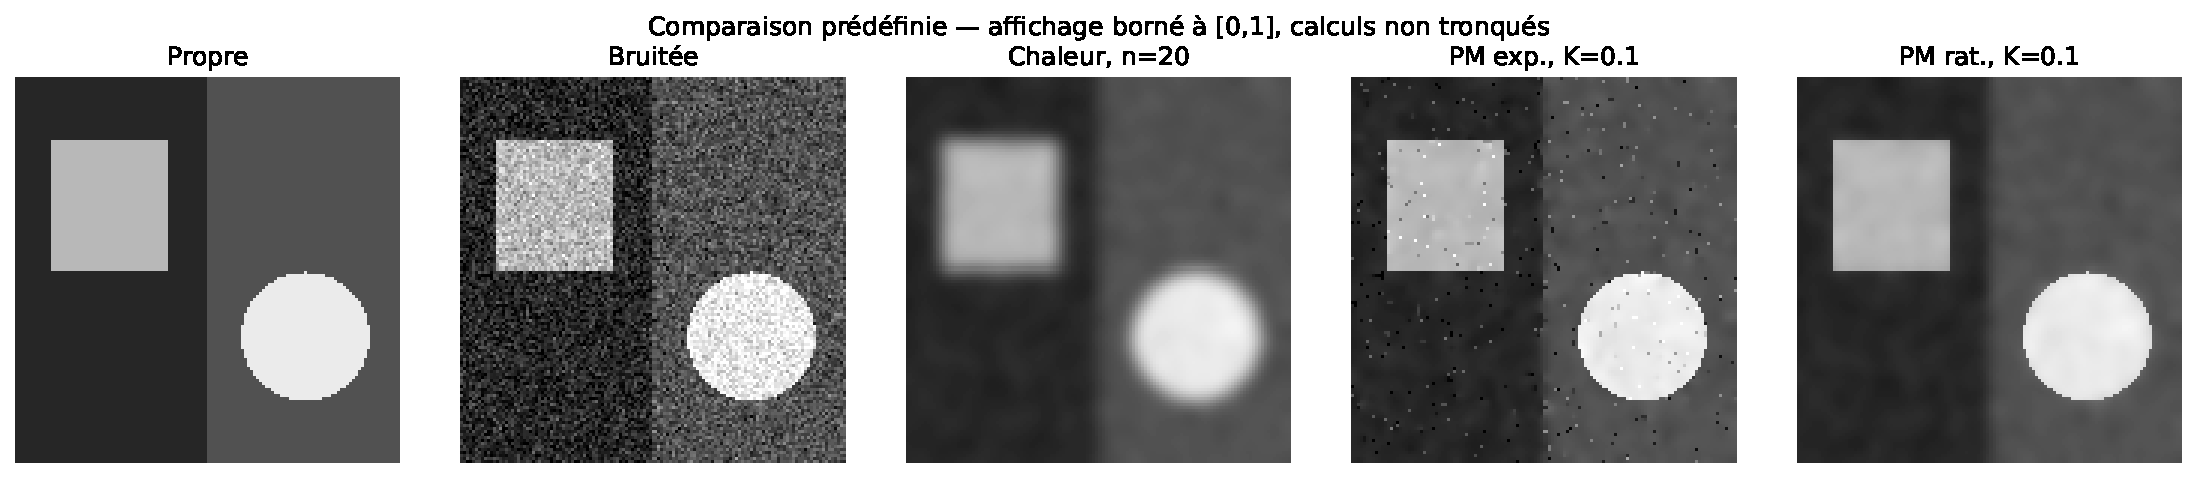
\includegraphics[width=\linewidth]{comparison.pdf}
 \caption{Cas individuel préfixé : \texttt{geometric\_shapes},
 $\sigma=0{,}10$, graine~$0$, $n=20$, $t=4$ ; $K=0{,}10$ pour les deux PM,
 $\dx=\dy=1$, $\dt=0{,}20$. Échelle d'affichage commune $[0,1]$,
 sans troncature des tableaux évalués. L'exponentielle conserve ici des
 fluctuations que la rationnelle atténue davantage ; aucune bande statistique.}
 \label{fig:comparison}
\end{figure}

Le profil de la figure~\ref{fig:profile} traverse le rectangle à la
ligne~$42$ (indices commençant à zéro). Contrairement aux images en gris,
il affiche les intensités non tronquées : les pics résiduels et la largeur
des transitions sont directement visibles. La figure~\ref{fig:gradients}
complète cette lecture par une visualisation de
$\sqrt{(D_xu)^2+(D_yu)^2}$ calculée avec \texttt{numpy.gradient}.
Ce gradient de visualisation n'est ni une métrique nouvelle ni le gradient
aux interfaces utilisé pour calculer les conductances directionnelles.
L'échelle colorée est commune ; son maximum est le plus grand des
$99$\textsuperscript{e} percentiles des cinq cartes, de sorte que certaines fortes
valeurs peuvent saturer à l'affichage sans être modifiées numériquement.

\begin{figure}[htbp]
 \centering
 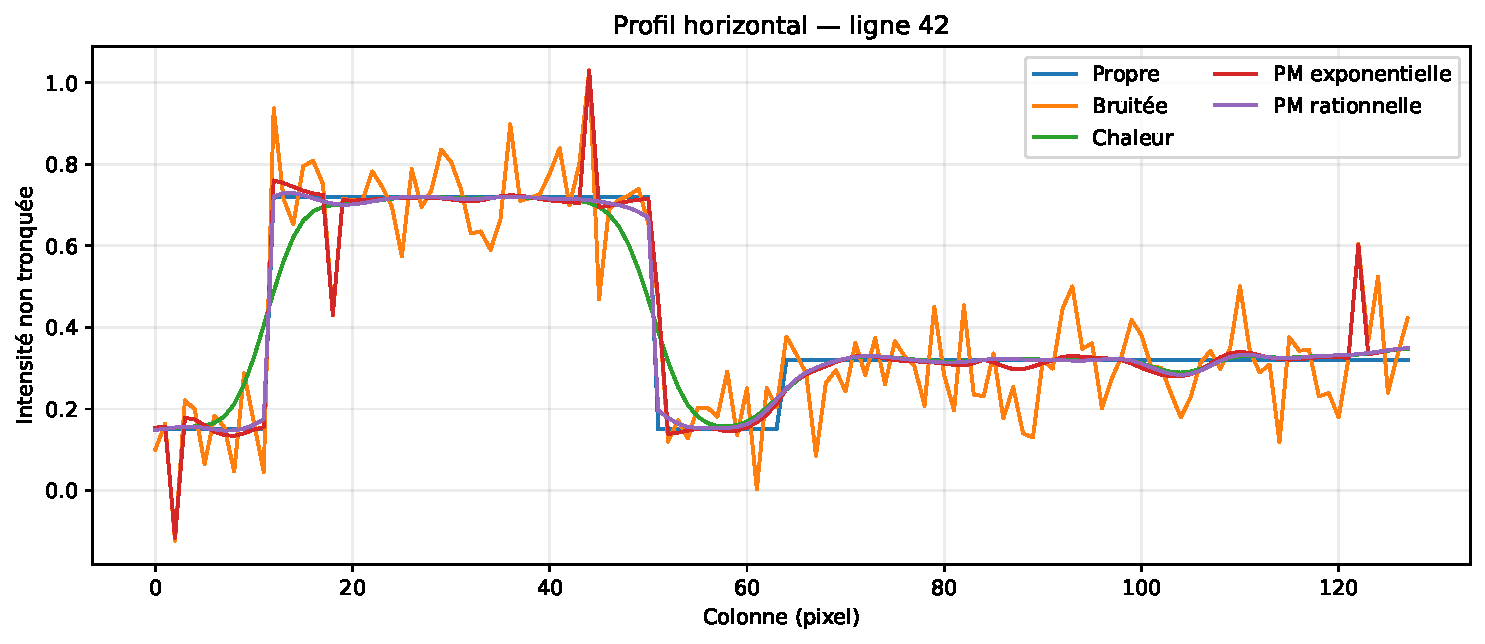
\includegraphics[width=0.95\linewidth]{intensity_profile.pdf}
 \caption{Profil horizontal, ligne~$42$, du même cas individuel
 \texttt{geometric\_shapes}, $\sigma=0{,}10$, graine~$0$, $n=20$, $t=4$,
 $K=0{,}10$, $\dx=\dy=1$, $\dt=0{,}20$. Intensités non tronquées :
 élargissement des transitions par la chaleur et pics résiduels de la PM
 exponentielle. Il ne s'agit pas d'une moyenne sur les graines.}
 \label{fig:profile}
\end{figure}
\begin{figure}[htbp]
 \centering
 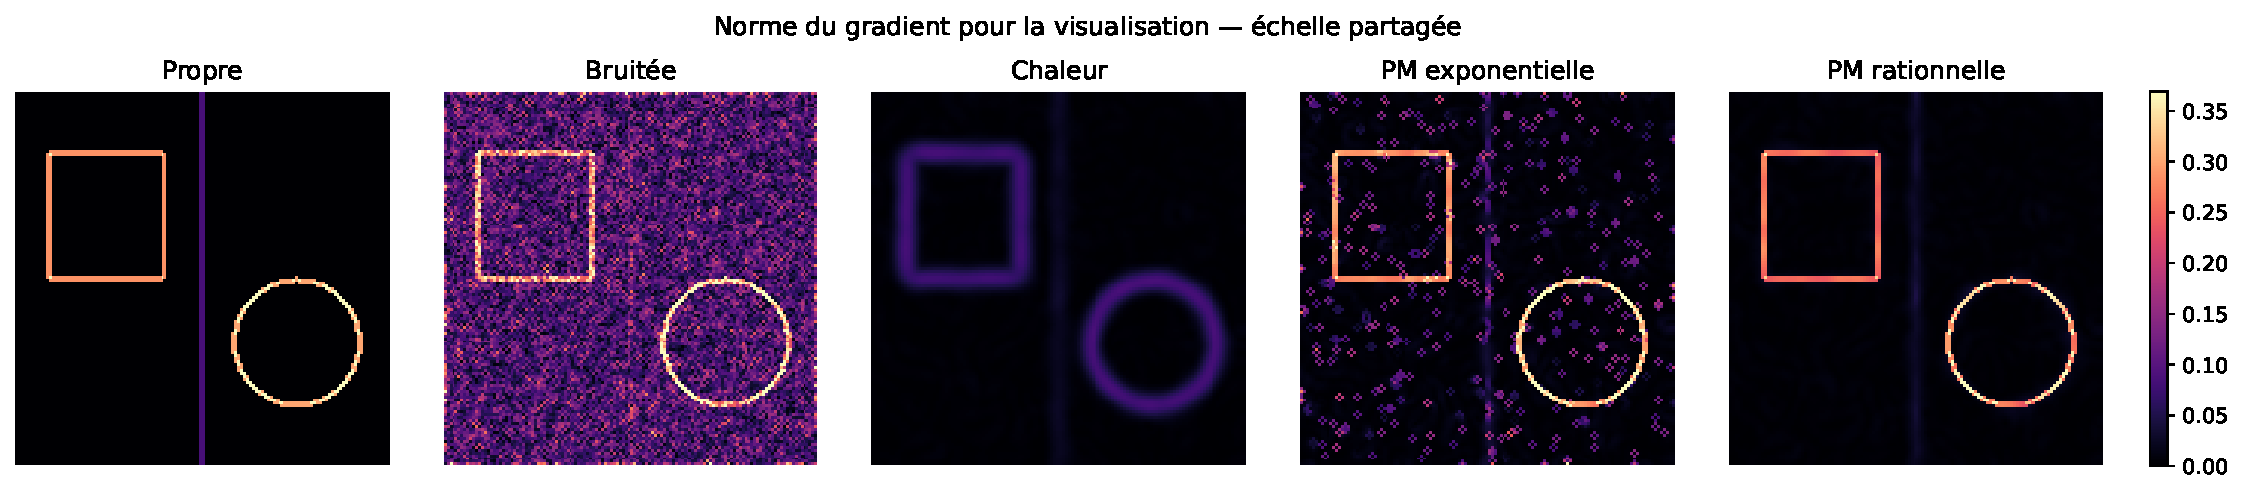
\includegraphics[width=\linewidth]{gradient_maps.pdf}
 \caption{Cartes de gradient du cas individuel \texttt{geometric\_shapes},
 $\sigma=0{,}10$, graine~$0$, $n=20$, $t=4$, $K=0{,}10$,
 $\dx=\dy=1$, $\dt=0{,}20$. Échelle commune, plafonnée pour l'affichage
 par les percentiles décrits dans le texte. Les réponses hors des frontières
 illustrent des fluctuations résiduelles ; ce n'est pas une mesure
 quantitative de qualité des contours.}
 \label{fig:gradients}
\end{figure}

Le tableau~\ref{tab:fixed-case}, lui, rapporte les dix graines.
La PM exponentielle améliore le PSNR par rapport à la chaleur
($28{,}3449$ contre $23{,}6482$~dB), tout en donnant un SSIM plus faible
($0{,}6254$ contre $0{,}8017$). L'erreur quadratique globale et les
statistiques structurelles locales ne classent donc pas nécessairement
les sorties de la même manière. La PM rationnelle avec ce $K$ atteint
ici les meilleurs scores des trois solveurs sélectionnés, sans que cette
comparaison à $K$ fixé désigne le meilleur réglage de toute la grille.

\begin{table}[htbp]
 \centering
 \caption{Comparaison agrégée fixée : \texttt{geometric\_shapes},
 $\sigma=0{,}10$, $n=20$, $t=4$, $K=0{,}10$ pour PM ; bruitée à $n=0$.
 Moyenne $\pm$ écart-type échantillonnal sur dix graines, non intervalle
 de confiance. Valeurs exportées depuis \texttt{summary.csv}.}
 \label{tab:fixed-case}
 % Generated from archived summary.csv; rounding applies only to display.
\begin{tabular}{lll}
\toprule
Méthode & PSNR (dB) & SSIM \\
\midrule
Bruitée & $19.9989 \pm 0.0458$ & $0.2168 \pm 0.0013$ \\
Chaleur & $23.6482 \pm 0.0432$ & $0.8017 \pm 0.0023$ \\
PM exp. & $28.3449 \pm 0.2351$ & $0.6254 \pm 0.0137$ \\
PM rat. & $34.6530 \pm 0.2974$ & $0.9292 \pm 0.0027$ \\
\bottomrule
\end{tabular}

\end{table}

\subsection{Toutes les valeurs de \texorpdfstring{$K$}{K} à budget commun}

Le tableau~\ref{tab:common-n20} conserve les huit variantes PM à $n=20$.
L'exponentielle avec $K=0{,}025$ reste proche de l'observation brute :
PSNR $20{,}1269$~dB, SSIM $0{,}2196$, contre $19{,}9989$~dB et $0{,}2168$
pour le bruit. Des différences dues au bruit dépassent elles aussi le
seuil, et leur diffusion devient très faible. Un petit $K$ ne distingue
donc pas automatiquement contour utile et fluctuation indésirable.
Avec $K=0{,}05$, l'exponentielle n'atteint encore que $21{,}1646$~dB.
Ces cas défavorables restent inclus, plutôt que supprimés au profit d'une
seule image flatteuse.

\begin{table}[htbp]
 \centering
 \caption{Toutes les méthodes à budget commun pour
 \texttt{geometric\_shapes}, $\sigma=0{,}10$, $n=20$, $t=4$ ;
 ligne bruitée de référence à $n=0$. Moyennes $\pm$ écarts-types
 échantillonnaux sur dix graines. $K=0{,}025$ est conservé exactement
 comme paramètre, sans arrondi en $0{,}03$.}
 \label{tab:common-n20}
 % Generated from archived summary.csv; rounding applies only to display.
\begin{tabular}{llrll}
\toprule
Méthode & $K$ & $n$ & PSNR (dB) & SSIM \\
\midrule
Chaleur & -- & 20 & $23.6482 \pm 0.0432$ & $0.8017 \pm 0.0023$ \\
Bruitée & -- & 0 & $19.9989 \pm 0.0458$ & $0.2168 \pm 0.0013$ \\
PM exp. & 0.025 & 20 & $20.1269 \pm 0.0483$ & $0.2196 \pm 0.0013$ \\
PM exp. & 0.05 & 20 & $21.1646 \pm 0.0617$ & $0.2455 \pm 0.0018$ \\
PM exp. & 0.1 & 20 & $28.3449 \pm 0.2351$ & $0.6254 \pm 0.0137$ \\
PM exp. & 0.2 & 20 & $35.7056 \pm 0.3280$ & $0.9378 \pm 0.0026$ \\
PM rat. & 0.025 & 20 & $23.7556 \pm 0.0893$ & $0.3276 \pm 0.0032$ \\
PM rat. & 0.05 & 20 & $33.3624 \pm 0.2979$ & $0.8348 \pm 0.0090$ \\
PM rat. & 0.1 & 20 & $34.6530 \pm 0.2974$ & $0.9292 \pm 0.0027$ \\
PM rat. & 0.2 & 20 & $26.9975 \pm 0.1527$ & $0.8667 \pm 0.0033$ \\
\bottomrule
\end{tabular}

\end{table}

\subsection{Temps de diffusion et sur-lissage}

Les figures~\ref{fig:curves025}--\ref{fig:curves10} couvrent les six cas.
Le suffixe image/bruit des fichiers identifie les agrégats sur dix
graines. Le fichier \texttt{metric\_curves.pdf} sans suffixe, qui concerne
uniquement la graine représentative, n'est pas utilisé comme courbe
agrégée. Chaque méthode dispose des mêmes checkpoints ; les bandes
expriment un écart-type, non une incertitude sur une population d'images.

\begin{figure}[p]
 \centering
 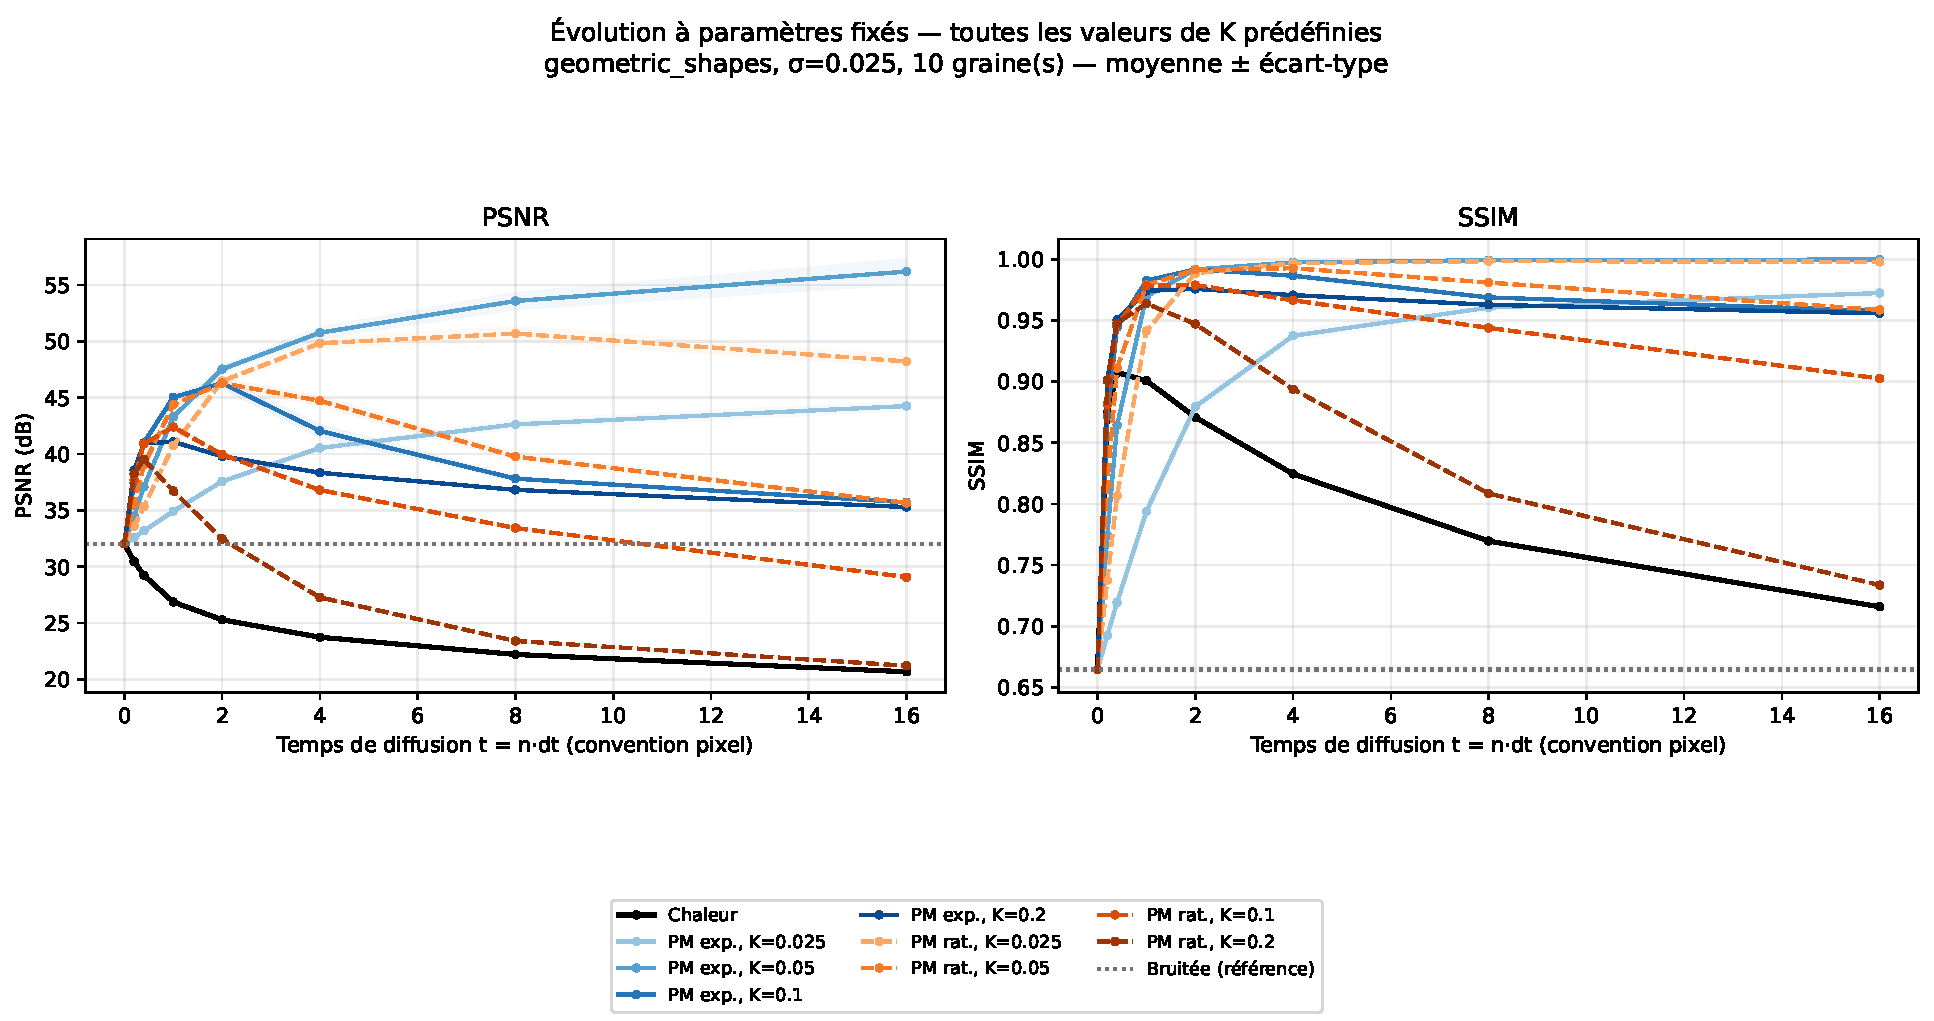
\includegraphics[width=0.98\linewidth]{metric_curves_geometric_shapes_sigma0p025.pdf}
 \par\medskip
 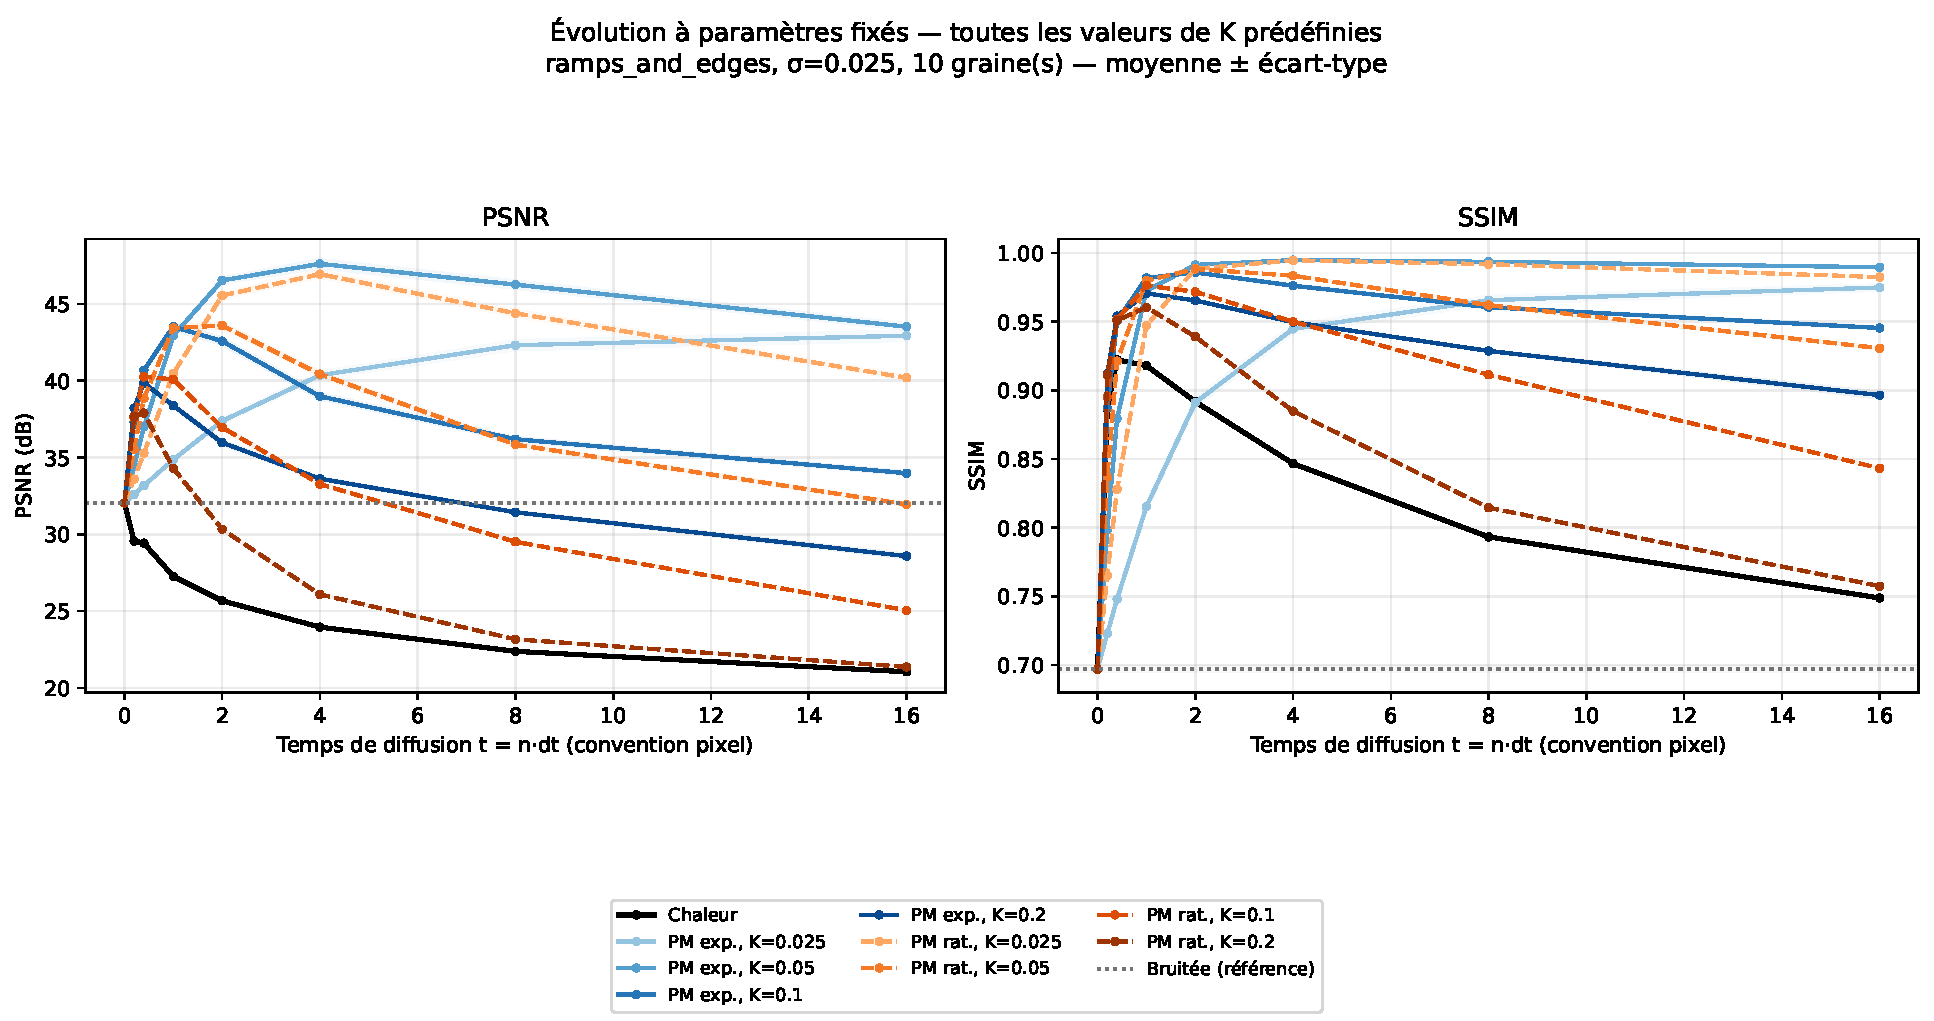
\includegraphics[width=0.98\linewidth]{metric_curves_ramps_and_edges_sigma0p025.pdf}
 \caption{PSNR et SSIM agrégés pour $\sigma=0{,}025$ :
 \texttt{geometric\_shapes} en haut, \texttt{ramps\_and\_edges} en bas.
 Moyennes sur dix graines ; bandes $\pm$ un écart-type échantillonnal.
 Chaleur et deux conductances PM, $K\in\{0{,}025;0{,}05;0{,}10;0{,}20\}$,
 $\dx=\dy=1$, $\dt=0{,}20$, $n=0,1,2,5,10,20,40,80$.
 Au faible bruit, un lissage plus intense peut dégrader la fidélité
 quadratique alors que les fluctuations locales diminuent.}
 \label{fig:curves025}
\end{figure}
\begin{figure}[p]
 \centering
 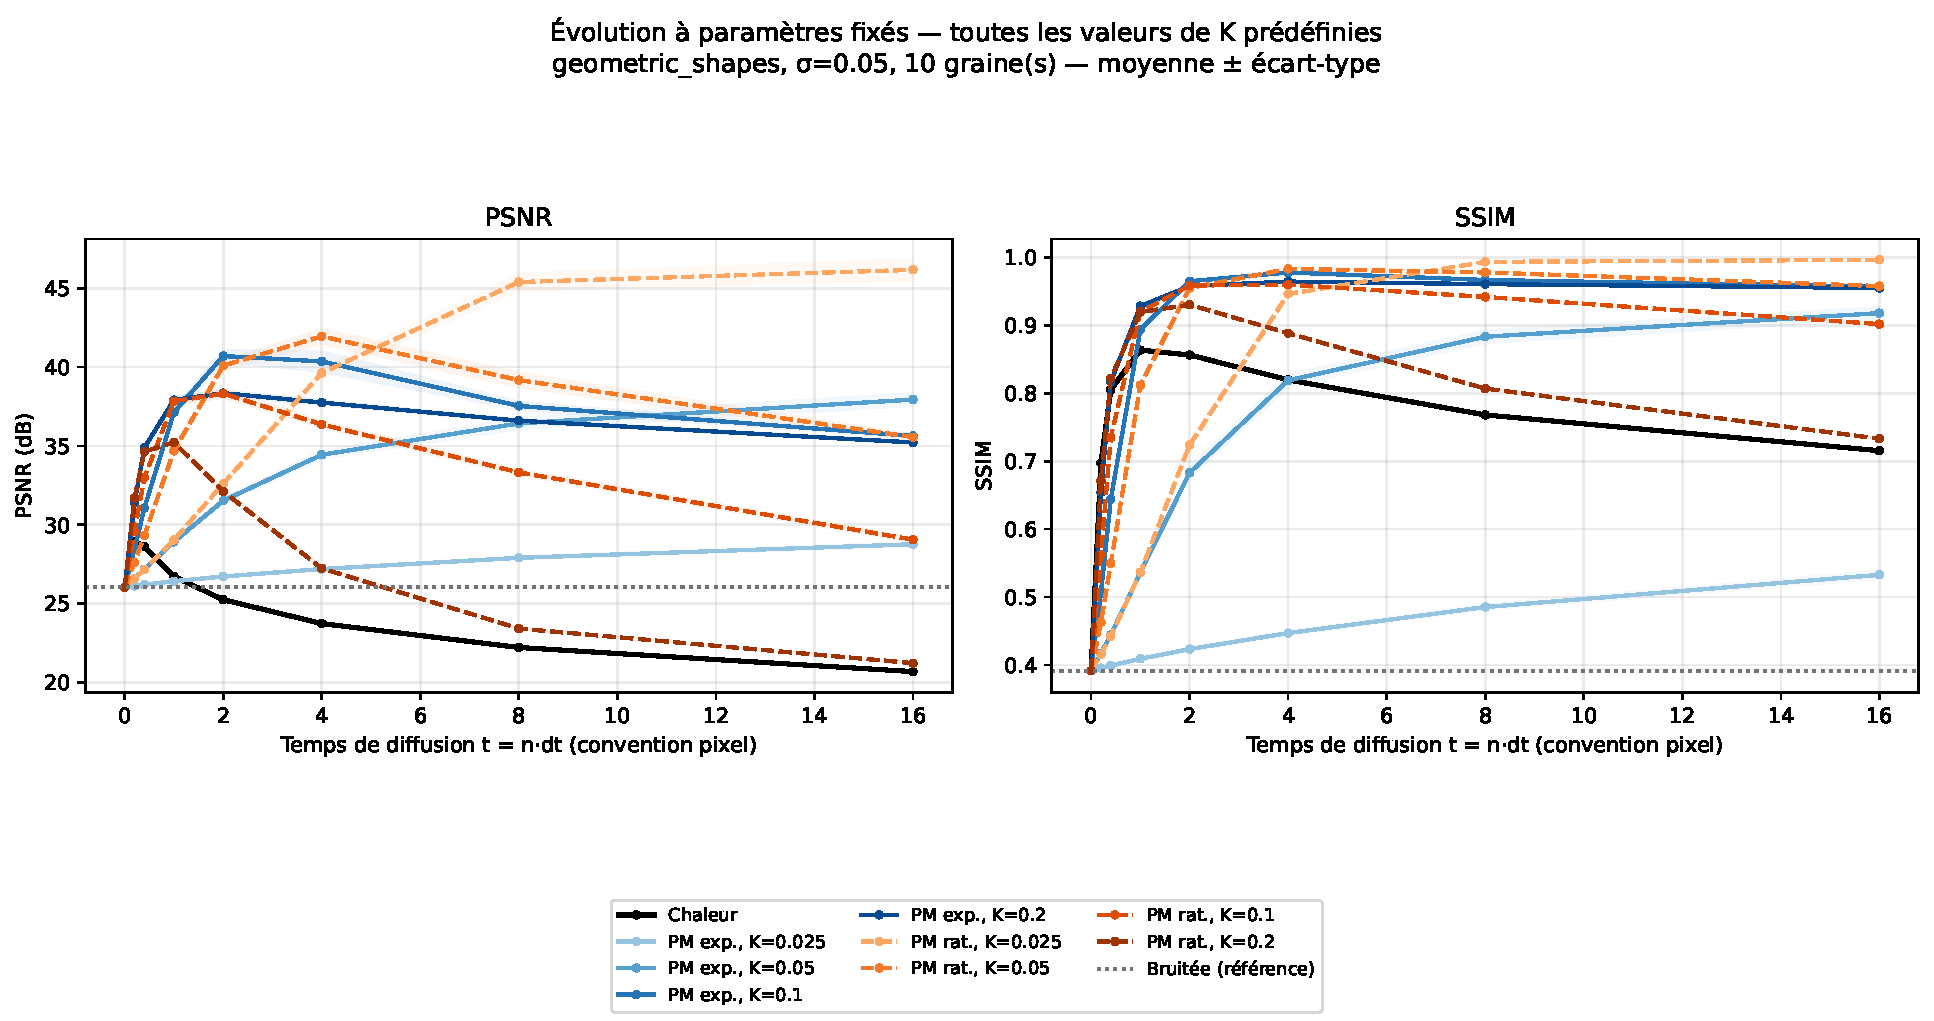
\includegraphics[width=0.98\linewidth]{metric_curves_geometric_shapes_sigma0p05.pdf}
 \par\medskip
 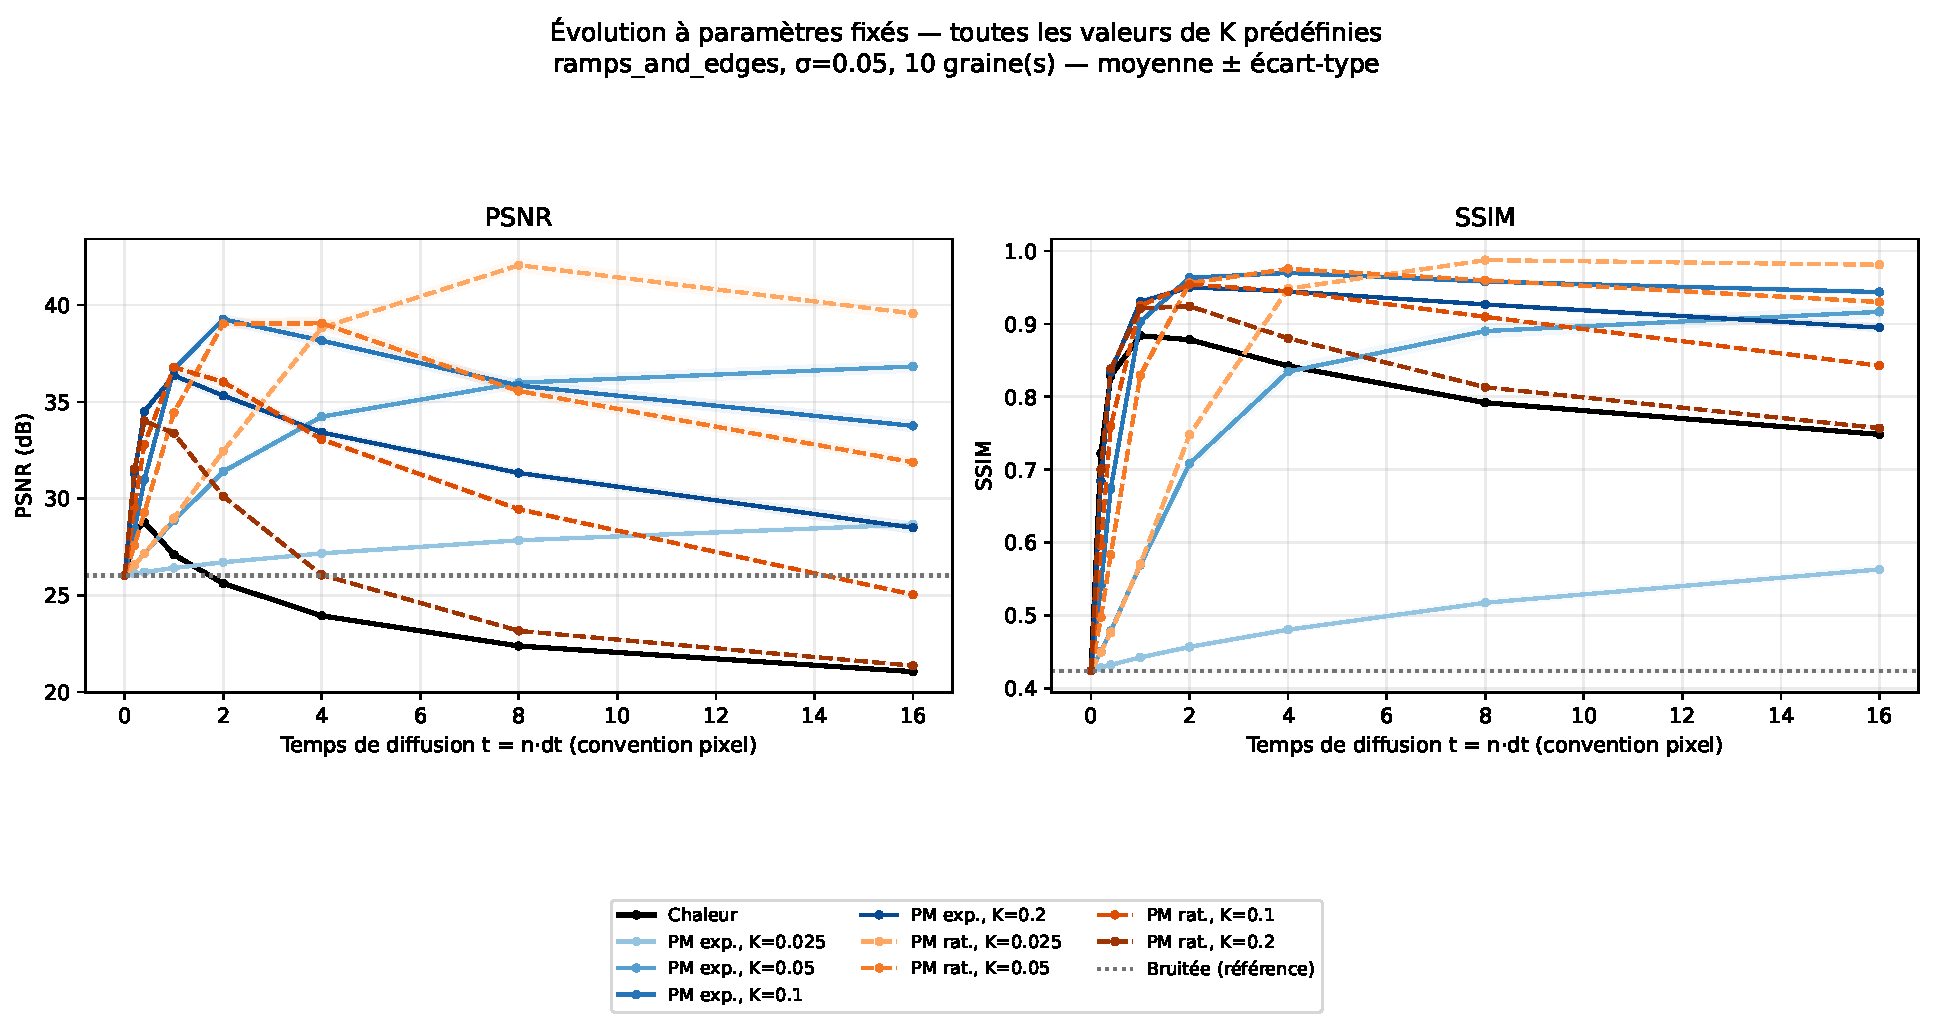
\includegraphics[width=0.98\linewidth]{metric_curves_ramps_and_edges_sigma0p05.pdf}
 \caption{PSNR et SSIM agrégés pour $\sigma=0{,}05$ :
 \texttt{geometric\_shapes} en haut, \texttt{ramps\_and\_edges} en bas.
 Dix graines, moyenne $\pm$ écart-type échantillonnal, non intervalle
 de confiance. Chaleur et PM exponentielle/rationnelle, quatre $K$
 prédéfinis de $0{,}025$ à $0{,}20$ ; $\dx=\dy=1$, $\dt=0{,}20$,
 checkpoints $0,1,2,5,10,20,40,80$. Les évolutions dépendent de la
 conductance et du seuil, et ne sont pas monotones pour toutes les variantes.}
 \label{fig:curves05}
\end{figure}
\begin{figure}[p]
 \centering
 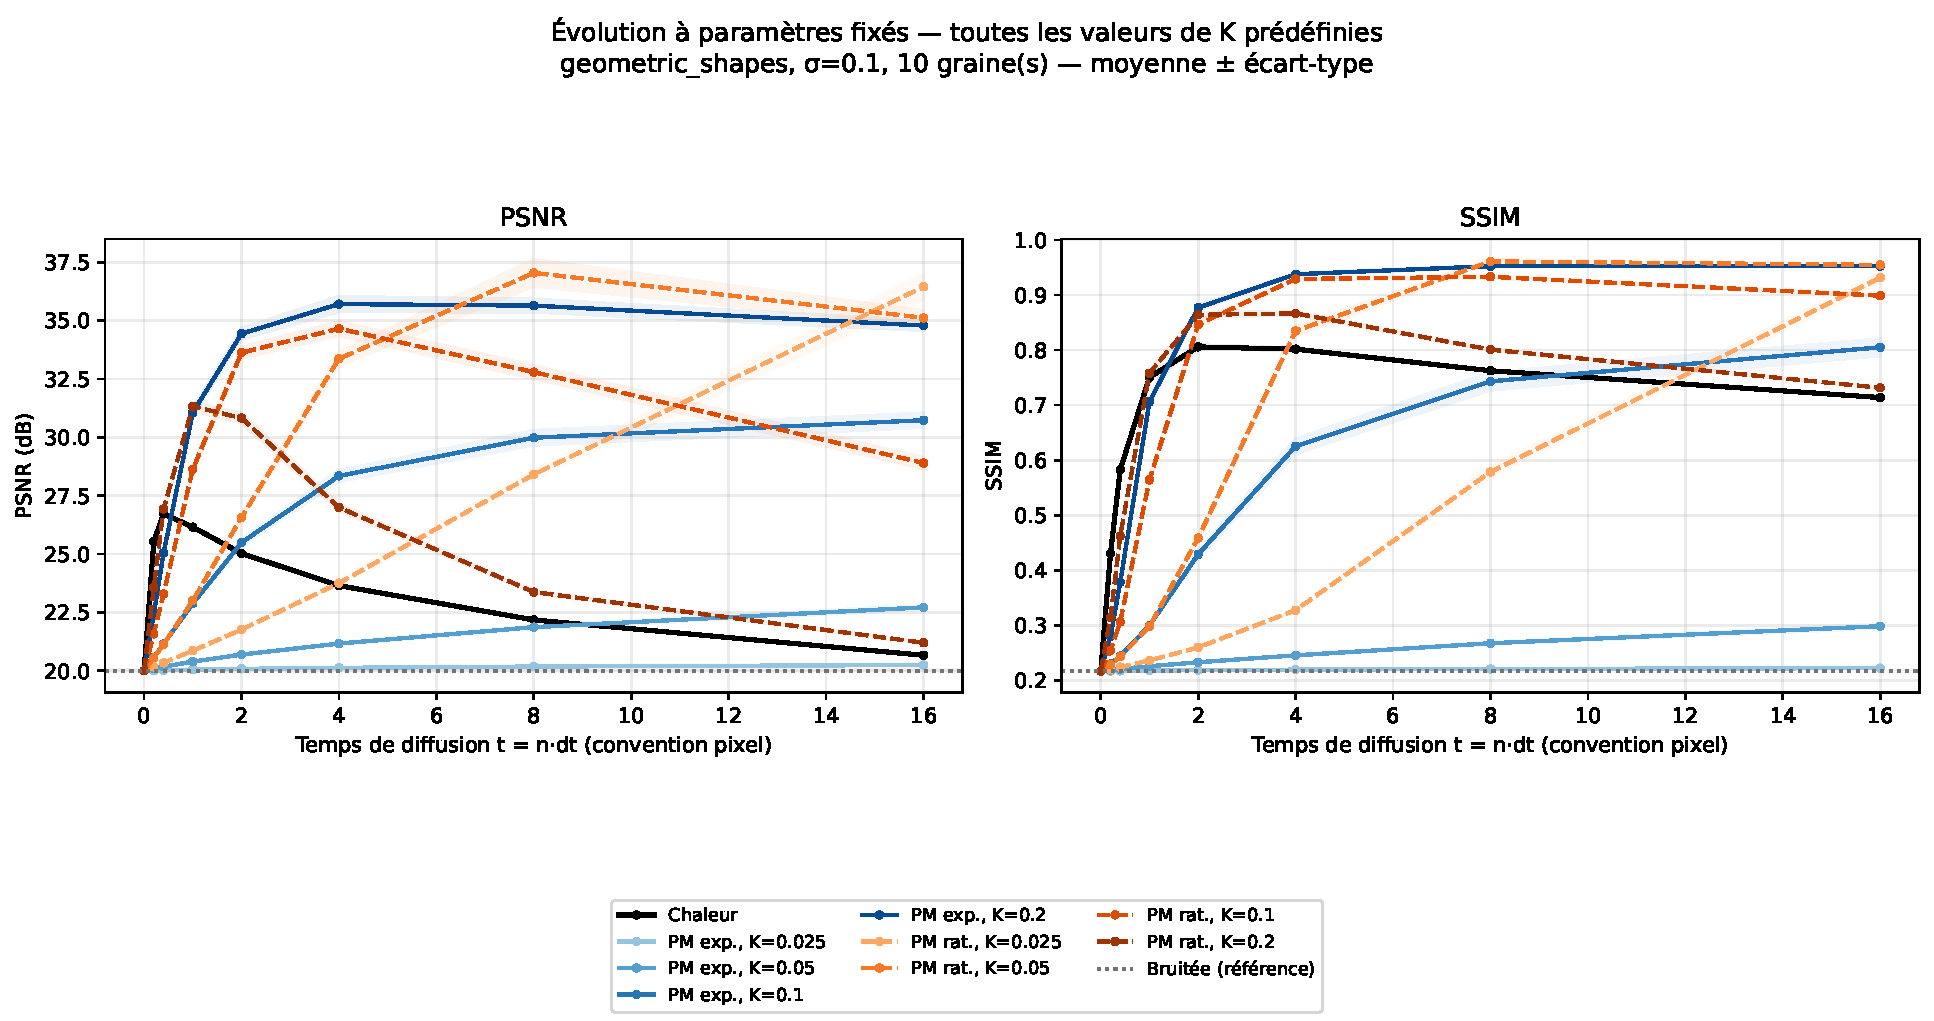
\includegraphics[width=0.98\linewidth]{metric_curves_geometric_shapes_sigma0p1.pdf}
 \par\medskip
 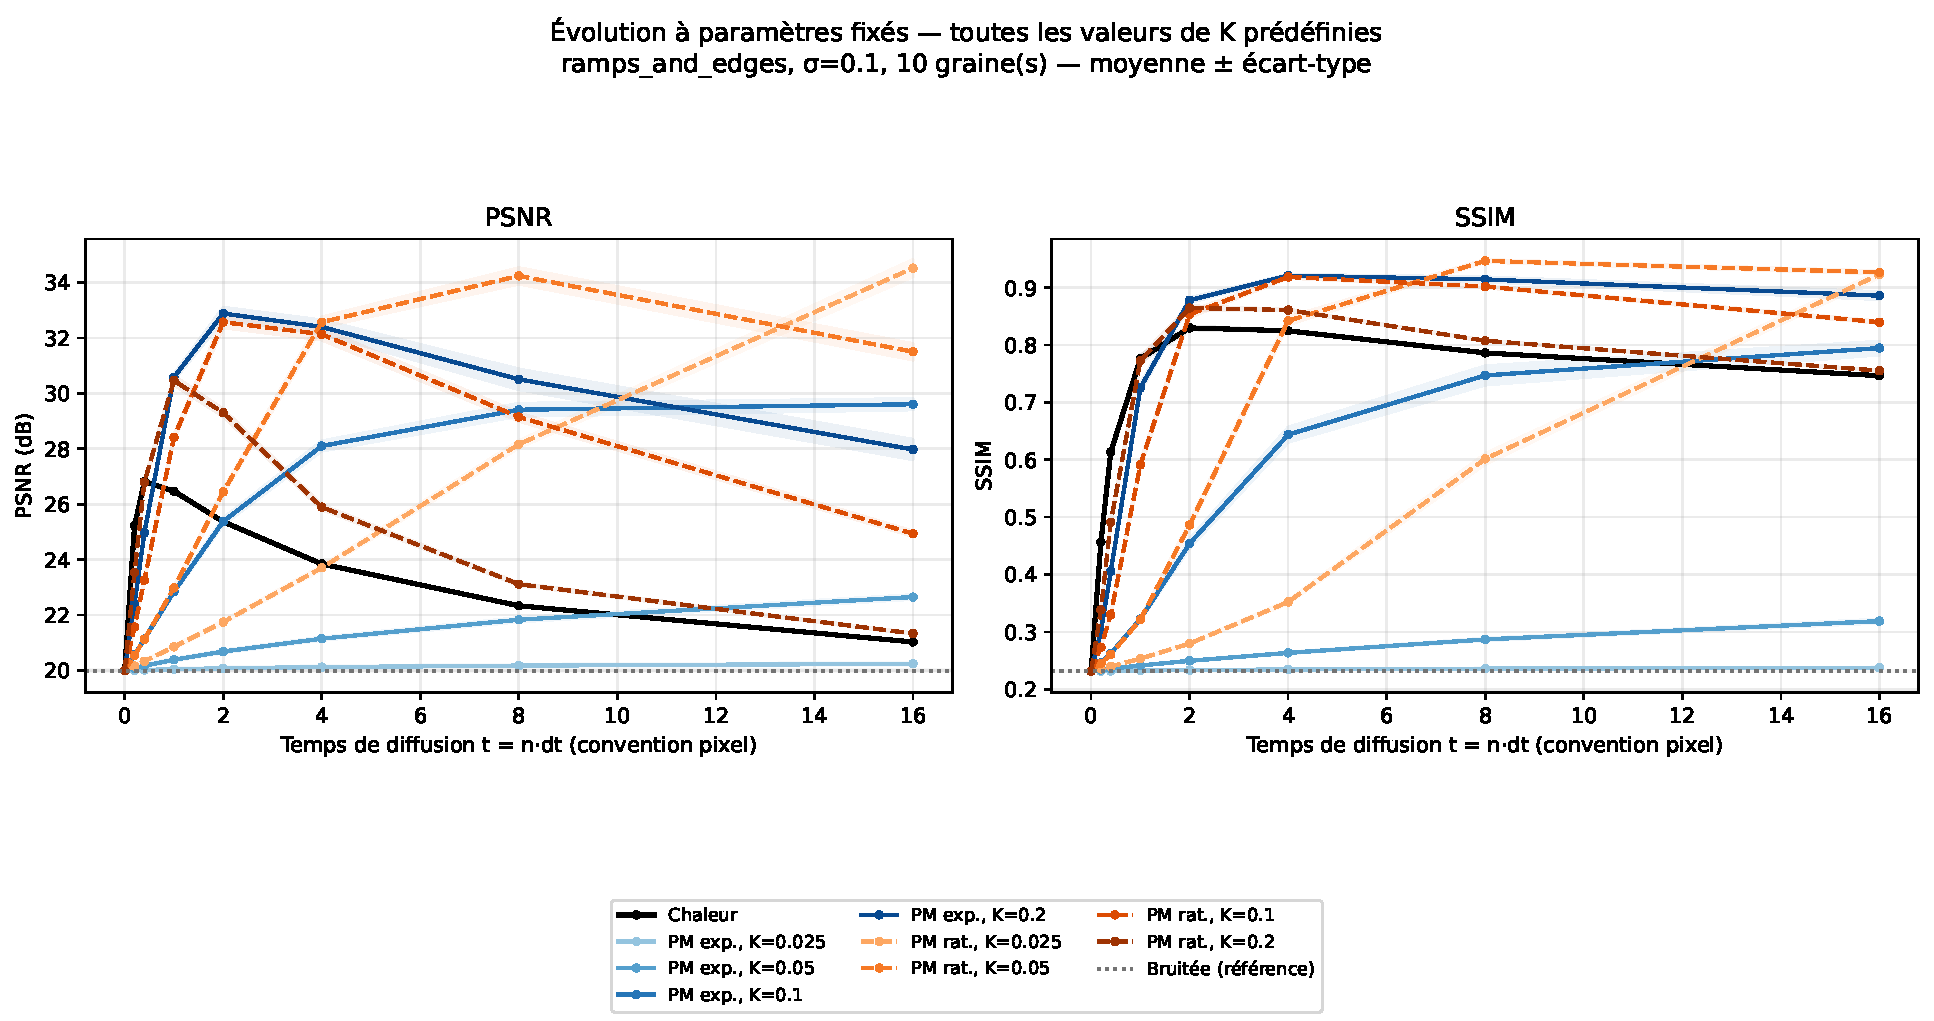
\includegraphics[width=0.98\linewidth]{metric_curves_ramps_and_edges_sigma0p1.pdf}
 \caption{PSNR et SSIM agrégés pour $\sigma=0{,}10$ :
 \texttt{geometric\_shapes} en haut, \texttt{ramps\_and\_edges} en bas.
 Moyennes et bandes $\pm$ un écart-type échantillonnal sur dix graines.
 Chaleur et huit PM avec $K=0{,}025;0{,}05;0{,}10;0{,}20$ ;
 $\dx=\dy=1$, $\dt=0{,}20$, huit checkpoints jusqu'à $t=16$.
 Les petits $K$ exponentiels conservent du bruit ; la poursuite des
 variantes plus diffusives peut conduire au sur-lissage.}
 \label{fig:curves10}
\end{figure}

Pour \texttt{geometric\_shapes}, $\sigma=0{,}10$, la chaleur atteint
$26{,}7244$~dB à $n=2$, mais seulement $20{,}6655$~dB à $n=80$.
Son SSIM passe de $0{,}8017$ à $n=20$ à $0{,}7138$ à $n=80$.
Le tableau~\ref{tab:time-case} montre que PM peut également sur-lisser :
la rationnelle $K=0{,}20$ passe de $31{,}3253$~dB à $n=5$ à
$21{,}1999$~dB à $n=80$. La stabilité n'implique donc pas que chaque
itération rapproche de la vérité terrain. Le schéma continue à diffuser,
mais les erreurs de structure peuvent prendre le dessus sur le gain
obtenu par réduction du bruit.

\begin{table}[htbp]
 \centering
 \caption{Interaction seuil/temps sur \texttt{geometric\_shapes},
 $\sigma=0{,}10$, aux checkpoints $n=2,5,20,80$ ($t=0{,}4;1;4;16$).
 Moyennes $\pm$ écarts-types échantillonnaux sur dix graines ;
 sous-ensemble explicite des variantes, sans budgets cachés.}
 \label{tab:time-case}
 % Generated from archived summary.csv; rounding applies only to display.
\begin{tabular}{llrll}
\toprule
Méthode & $K$ & $n$ & PSNR (dB) & SSIM \\
\midrule
Chaleur & -- & 2 & $26.7244 \pm 0.0724$ & $0.5828 \pm 0.0054$ \\
Chaleur & -- & 5 & $26.1523 \pm 0.0636$ & $0.7506 \pm 0.0064$ \\
Chaleur & -- & 20 & $23.6482 \pm 0.0432$ & $0.8017 \pm 0.0023$ \\
Chaleur & -- & 80 & $20.6655 \pm 0.0337$ & $0.7138 \pm 0.0009$ \\
PM exp. & 0.2 & 2 & $25.0458 \pm 0.0954$ & $0.3783 \pm 0.0040$ \\
PM exp. & 0.2 & 5 & $31.0611 \pm 0.1795$ & $0.7061 \pm 0.0084$ \\
PM exp. & 0.2 & 20 & $35.7056 \pm 0.3280$ & $0.9378 \pm 0.0026$ \\
PM exp. & 0.2 & 80 & $34.7866 \pm 0.2153$ & $0.9525 \pm 0.0008$ \\
PM rat. & 0.1 & 2 & $23.2927 \pm 0.0720$ & $0.3063 \pm 0.0024$ \\
PM rat. & 0.1 & 5 & $28.6326 \pm 0.1392$ & $0.5643 \pm 0.0067$ \\
PM rat. & 0.1 & 20 & $34.6530 \pm 0.2974$ & $0.9292 \pm 0.0027$ \\
PM rat. & 0.1 & 80 & $28.8937 \pm 0.2417$ & $0.8988 \pm 0.0023$ \\
PM rat. & 0.2 & 2 & $26.9275 \pm 0.0986$ & $0.4623 \pm 0.0041$ \\
PM rat. & 0.2 & 5 & $31.3253 \pm 0.1804$ & $0.7580 \pm 0.0066$ \\
PM rat. & 0.2 & 20 & $26.9975 \pm 0.1527$ & $0.8667 \pm 0.0033$ \\
PM rat. & 0.2 & 80 & $21.1999 \pm 0.0396$ & $0.7315 \pm 0.0010$ \\
\bottomrule
\end{tabular}

\end{table}

La figure~\ref{fig:k-sensitivity} compare les deux conductances aux
mêmes $K$ et aux mêmes temps. La rationnelle $K=0{,}025$, sur le premier
cas à $\sigma=0{,}10$, atteint $23{,}7556$~dB à $n=20$ puis
$36{,}4457$~dB à $n=80$ : un petit seuil peut demander un temps plus long
et n'est pas intrinsèquement défavorable. En revanche, augmenter $K$
favorise une diffusion plus forte et peut nécessiter un arrêt plus tôt.
Une comparaison de seuils détachée de la conductance et du temps serait
donc incomplète.

\begin{figure}[p]
 \centering
 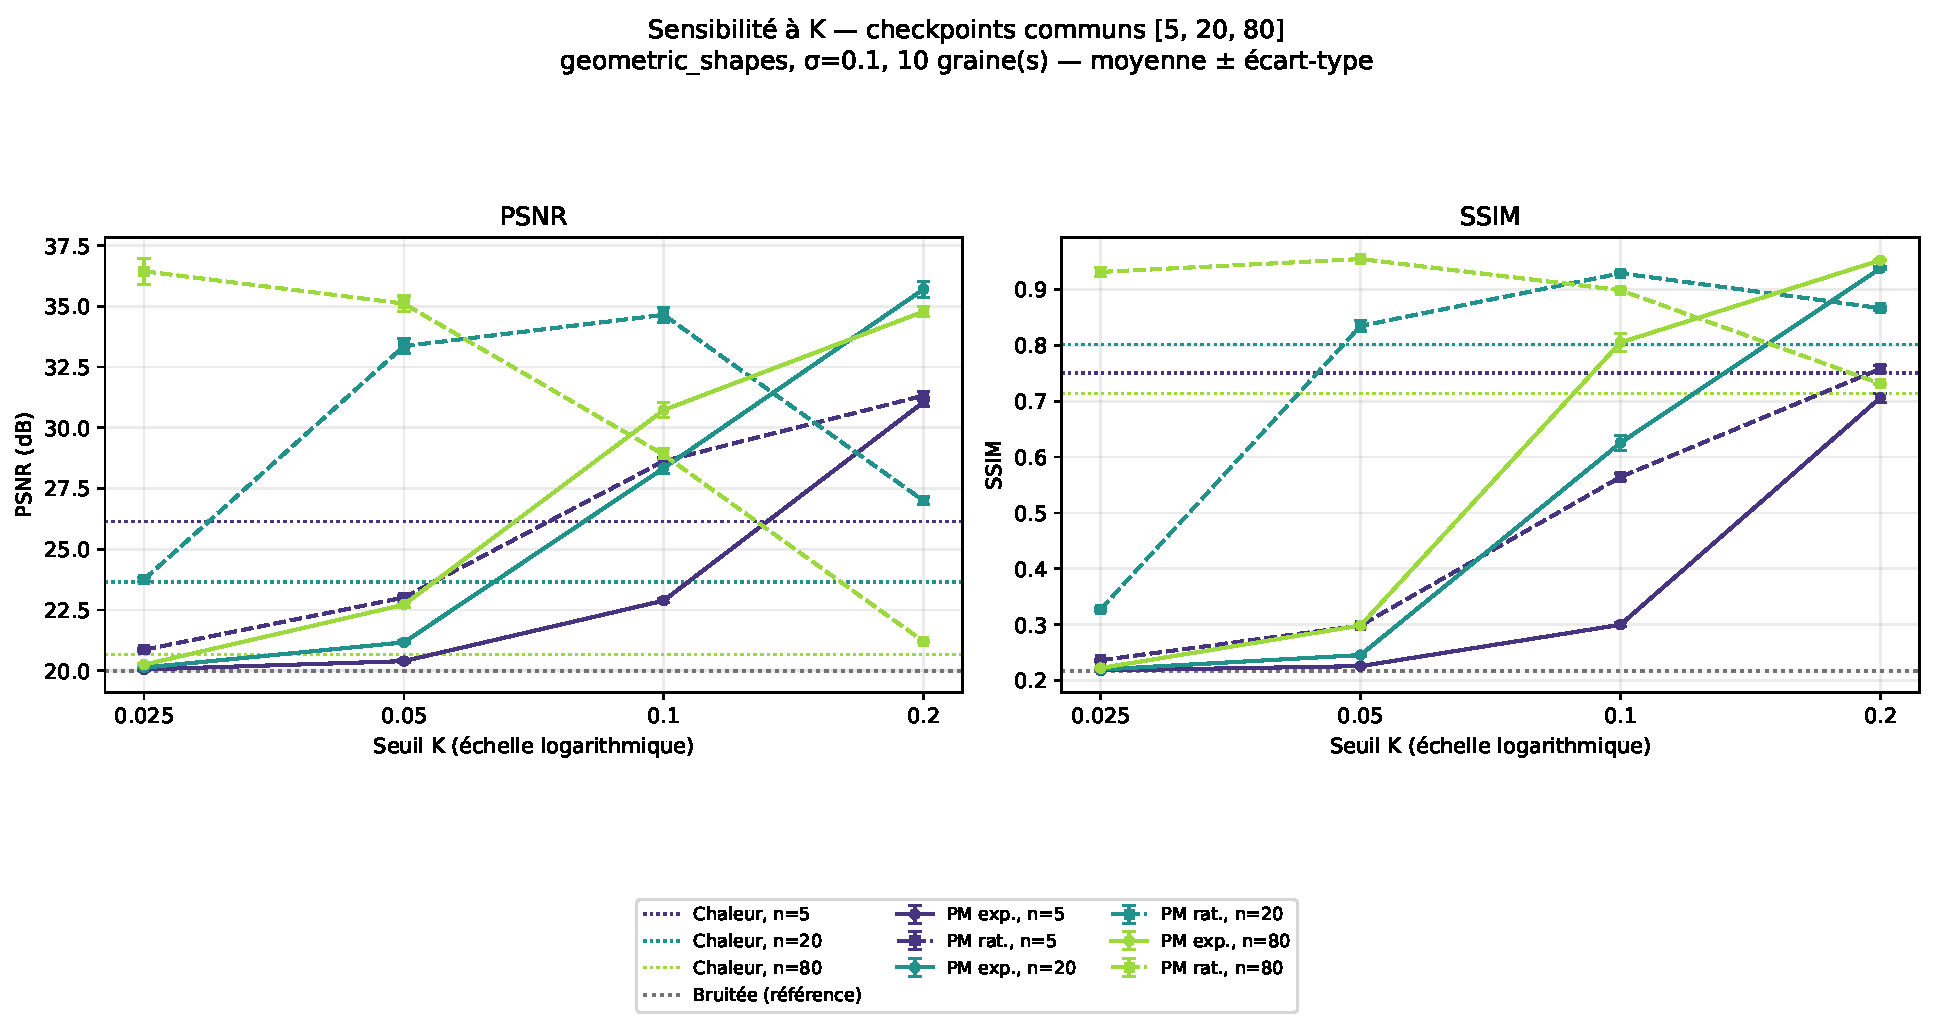
\includegraphics[width=0.98\linewidth]{k_sensitivity_geometric_shapes_sigma0p1.pdf}
 \par\medskip
 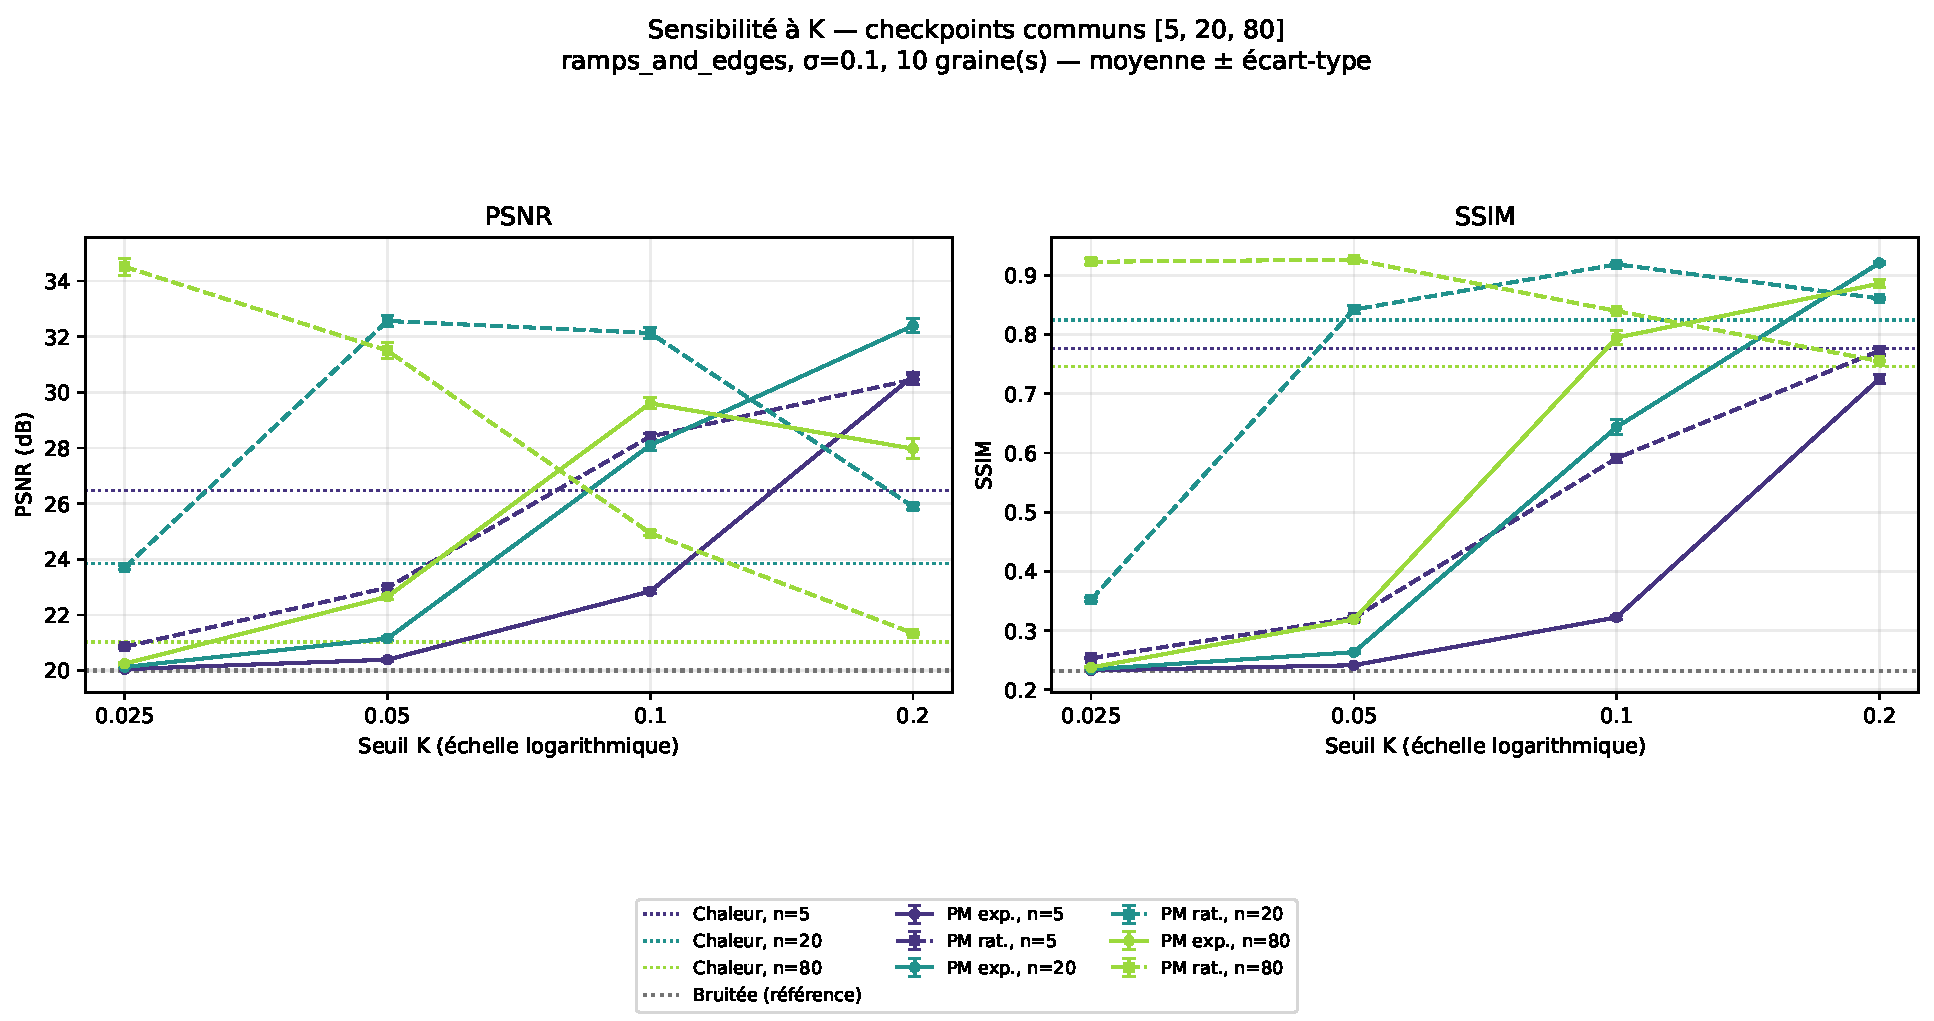
\includegraphics[width=0.98\linewidth]{k_sensitivity_ramps_and_edges_sigma0p1.pdf}
 \caption{Sensibilité à $K$ pour $\sigma=0{,}10$ :
 \texttt{geometric\_shapes} en haut, \texttt{ramps\_and\_edges} en bas.
 Deux conductances, $n=5,20,80$ ($t=1,4,16$),
 $K=0{,}025;0{,}05;0{,}10;0{,}20$, $\dx=\dy=1$, $\dt=0{,}20$.
 Points : moyennes sur dix graines ; barres : un écart-type échantillonnal.
 Les références de chaleur sont aux mêmes checkpoints. L'évolution avec
 $K$ change avec le temps : aucun seuil universel n'est identifié.}
 \label{fig:k-sensitivity}
\end{figure}

\subsection{Désaccords entre critères}

Le cas fixé n'est pas isolé. À $\sigma=0{,}025$ sur
\texttt{geometric\_shapes}, une seule itération de chaleur réduit le
PSNR moyen de $32{,}0401$ à $30{,}4691$~dB, mais augmente le SSIM de
$0{,}6646$ à $0{,}8740$. Sur \texttt{ramps\_and\_edges},
$\sigma=0{,}10$, $n=20$, la rationnelle $K=0{,}05$ donne
$32{,}5651\pm0{,}1841$~dB et $0{,}8422\pm0{,}0070$ en SSIM ;
l'exponentielle $K=0{,}20$ donne $32{,}3930\pm0{,}2530$~dB et
$0{,}9209\pm0{,}0023$. Les dispersions invitent à ne pas surinterpréter
le faible écart de PSNR ; les moyennes inversent leur ordre selon le critère,
sans qu'un test de significativité soit effectué ici.

Sur les $42$ couples cas/checkpoint positif, le meilleur réglage selon
le PSNR moyen et celui selon le SSIM moyen diffèrent $13$ fois.
Le compte rendu \texttt{analysis.json} relève aussi $172$ paires
discordantes sur $1\,512$ comparaisons de paires sans égalité.
Ces comptes décrivent la grille, sans test statistique. Enfin,
l'exponentielle $K=0{,}20$ sur \texttt{geometric\_shapes},
$\sigma=0{,}10$, passe entre $n=20$ et $80$ de $35{,}7056$ à
$34{,}7866$~dB, tandis que son SSIM augmente de $0{,}9378$ à $0{,}9525$.
Même le choix d'arrêt peut donc dépendre du critère.

\subsection{Meilleurs réglages observés : un oracle exploratoire}

Le tableau~\ref{tab:oracle-psnr} maximise le PSNR \emph{moyen sur les dix
graines}, parmi les configurations de solveur et checkpoints $n>0$
prédéfinis. C'est un \emph{oracle exploratoire}, puisqu'il utilise
l'image propre. Ce n'est ni un réglage sélectionnable sur une observation
seule ni une performance de généralisation. Il ne maximise pas
séparément chaque graine avant de moyenner : la règle de sélection doit
rester explicite.

\begin{table}[htbp]
 \centering
 \caption{Oracle exploratoire PSNR : maximum de la moyenne sur dix
 graines, parmi la grille figée avec $n>0$. Images et bruits indiqués
 dans chaque ligne ; dispersions échantillonnales. Tout $n=80$ est
 à la frontière temporelle étudiée, pas un optimum global.}
 \label{tab:oracle-psnr}
 % Generated from archived summary.csv; rounding applies only to display.
\begin{tabular}{lllrll}
\toprule
Image / $\sigma$ & Méthode & $K$ & $n$ & PSNR (dB) & SSIM \\
\midrule
Géométrique / 0.025 & PM exp. & 0.05 & 80 & $56.2055 \pm 1.0724$ & $0.9998 \pm 4.10\times10^{-5}$ \\
Géométrique / 0.05 & PM rat. & 0.025 & 80 & $46.1862 \pm 0.6477$ & $0.9967 \pm 0.0004$ \\
Géométrique / 0.1 & PM rat. & 0.05 & 40 & $37.0422 \pm 0.5734$ & $0.9611 \pm 0.0035$ \\
Rampe / 0.025 & PM exp. & 0.05 & 20 & $47.6194 \pm 0.2821$ & $0.9948 \pm 0.0004$ \\
Rampe / 0.05 & PM rat. & 0.025 & 40 & $42.0671 \pm 0.2953$ & $0.9874 \pm 0.0009$ \\
Rampe / 0.1 & PM rat. & 0.025 & 80 & $34.5137 \pm 0.3117$ & $0.9229 \pm 0.0053$ \\
\bottomrule
\end{tabular}

\end{table}

Les choix PSNR/SSIM coïncident dans cinq des six cas. Pour
\texttt{ramps\_and\_edges}, $\sigma=0{,}10$, l'oracle SSIM est en
revanche la rationnelle $K=0{,}05$, $n=40$, alors que l'oracle PSNR
choisit $K=0{,}025$, $n=80$ (tableau~\ref{tab:oracle-difference}).
Plusieurs maxima sont à $n=80$ ; aucun résultat ne permet de les appeler
optima globaux en temps, et aucune expérience supplémentaire n'est
introduite pour prolonger les courbes.

\begin{table}[htbp]
 \centering
 \caption{Deux oracles exploratoires distincts pour
 \texttt{ramps\_and\_edges}, $\sigma=0{,}10$ : sélection selon PSNR ou
 SSIM moyen. Dix graines ; scores et écarts-types issus du CSV,
 $\dx=\dy=1$, $\dt=0{,}20$.}
 \label{tab:oracle-difference}
 % Generated from archived summary.csv; rounding applies only to display.
\begin{tabular}{llrll}
\toprule
Méthode & $K$ & $n$ & PSNR (dB) & SSIM \\
\midrule
PM rat. & 0.025 & 80 & $34.5137 \pm 0.3117$ & $0.9229 \pm 0.0053$ \\
PM rat. & 0.05 & 40 & $34.2340 \pm 0.2965$ & $0.9465 \pm 0.0025$ \\
\bottomrule
\end{tabular}

\end{table}

\chapter{Reproductibilité, limites et conclusion}
\section{Reproductibilité : fichiers, nombres et temps machine}
\label{sec:reproducibility}

\subsection{Environnement enregistré et formats}

Le calcul étendu a été exécuté sur CPU sous Windows, dans l'environnement
Python local du projet, avec tableaux NumPy \texttt{float64}. Les versions
du tableau~\ref{tab:environment} proviennent du fichier
\path{environment.json}, et non de versions supposées disponibles au
moment de la lecture du rapport. Le paquet porte la version interne
$0.0.0$, qui n'est pas une publication.

\begin{table}[htbp]
 \centering
 \caption{Environnement du calcul étendu archivé ; versions enregistrées,
 sans installation ni nouvelle expérience pour la rédaction.}
 \label{tab:environment}
 \begin{tabular}{ll}
\toprule
Élément & Valeur enregistrée \\
\midrule
Python & 3.14.6 \\
Plateforme & Windows-11-10.0.26200-SP0 \\
numpy & 2.5.3 \\
matplotlib & 3.11.2 \\
pytest & 9.1.1 \\
pde-image-denoising & 0.0.0 \\
Calcul & CPU, float64 \\
\bottomrule
\end{tabular}

\end{table}

Une tentative initiale d'import de \path{skimage.metrics} avait chargé
une DLL SciPy refusée par Windows Application Control. La restriction
n'a pas été contournée. Les mesures finales utilisent donc les formules
NumPy documentées en section~\ref{sec:metrics} ; les paquets optionnels
\texttt{scikit-image} et SciPy, présents après cette tentative, ne sont
pas utilisés par le calcul. Cette différence d'implémentation est
consignée pour éviter une attribution trompeuse à une bibliothèque.

Chaque ligne de \path{metrics.csv} identifie image, bruit, graine,
méthode, conductance, $K$, pas, checkpoint, temps de diffusion, quatre
scores et durée cumulative. Des hashes identifient les observations et
sorties. \path{summary.csv} regroupe sans perdre la définition des
métriques individuelles. Les fichiers NPZ archivent les entrées et les
sorties nécessaires aux exemples ; les PDF/PNG, tables, configuration,
environnement, journal et manifeste complètent la chaîne de provenance.

\subsection{Intégrité et modes de vérification}

Le manifeste énumère les fichiers de résultats, leurs tailles et SHA-256,
et relie la configuration utilisée à son empreinte. Les hashes d'arrays
sont calculés sur une représentation canonique \texttt{float64} de
boutisme fixé, avec forme et type inclus. Le vérificateur contrôle la
structure des CSV, les clés de regroupement, les graines, les observations
communes, les métriques recalculées et toutes les moyennes et dispersions.
Les statistiques de durée sont recalculées depuis les durées enregistrées,
jamais comparées à un nouveau chronométrage.

Deux constats doivent être distingués. Le compte rendu local archivé
\path{results/extended/verification.json} atteste une reproduction
\emph{stricte} dans l'environnement Windows enregistré : égalité exacte
et aucune différence de hash recalculé. L'audit indépendant communiqué
pour cette phase atteste une reproduction \emph{numérique}
inter-environnements, avec \texttt{rtol=1e-10} et \texttt{atol=1e-12}.
Ce second constat est celui de l'audit fourni, et non une vérification
relancée pendant la rédaction.

Le mode numérique conserve des contrôles exacts de structure et
d'intégrité des fichiers archivés, mais accepte de faibles différences
des quantités recalculées sous la règle
$|a-b|\leq10^{-12}+10^{-10}|b|$. Il signale leurs éventuels hashes
différents sans annoncer une reproduction exacte. L'intégrité d'un
ZIP ou d'un manifeste et la proximité numérique entre environnements
sont donc deux garanties différentes. Le tableau~\ref{tab:verification}
résume les contrôles locaux réellement enregistrés ; les $165$ tests
réussis appartiennent à la validation antérieure, sans relance de la
suite scientifique pour cette rédaction.

\begin{table}[htbp]
 \centering
 \caption{Contrôles consignés dans la vérification stricte locale de
 phase~4 ; durée et horodatage ne sont pas assimilés à des quantités
 déterministes.}
 \label{tab:verification}
 \begin{tabular}{lll}
\toprule
Contrôle & Niveau & Erreur d'amplitude ou maximale \\
\midrule
Mode propre discret & $17\times19$, 7 pas & $3.60822483\times10^{-16}$ \\
Spatial & 16 & $5.20069556\times10^{-4}$ \\
Spatial & 32 & $1.30111858\times10^{-4}$ \\
Temporel & 8 & $1.43420373\times10^{-4}$ \\
Temporel & 16 & $7.15660884\times10^{-5}$ \\
\bottomrule
\end{tabular}

\end{table}

\subsection{Lire correctement les durées}

La durée enregistrée du pipeline expérimental est
$44{,}407302$~s dans son environnement d'origine. Elle inclut calculs,
métriques, écritures et figures ; elle n'est pas une mesure universelle
de coût. La somme des durées \emph{terminales} des $540$ trajectoires
est $16{,}5264453$~s. Le chronométrage du solveur inclut les copies
d'états aux checkpoints, mais pas la génération du bruit, les métriques,
les hashes ou les figures. Les durées aux checkpoints sont cumulatives :
les additionner sur tous les checkpoints compterait plusieurs fois le
même calcul. Enfin, $t=n\dt$ est un temps de diffusion dans une convention
numérique, sans relation d'identité avec ces secondes machine.

\section{Portée des résultats, limites et perspectives}
\label{sec:discussion}

\subsection{Réponse conditionnelle à la question de comparaison}

La diffusion dépendant des variations locales modifie effectivement le
compromis entre réduction du bruit et maintien de structures dans la
grille étudiée, mais cette modification dépend du seuil, de la conductance,
du temps et du critère. Au cas fixé, la rationnelle $K=0{,}10$ obtient
de meilleurs PSNR et SSIM que la chaleur à $n=20$. L'exponentielle au
même seuil améliore seulement le premier de ces deux critères.
À faible $K$, la limitation des flux peut aussi conserver le bruit ;
à forte diffusion ou après trop d'itérations, PM comme la chaleur peut
sur-lisser. Le gain potentiel n'est donc pas une propriété inconditionnelle
du nom de la méthode.

Ces observations sont compatibles avec le mécanisme des flux, sans
valoir démonstration d'une théorie de performance. La conservation de
la moyenne et le principe du maximum concernent l'évolution discrète
elle-même ; la fidélité à une image propre donnée relève d'une autre
question. Une évolution qui reste bornée entre les extrema de l'entrée
peut néanmoins éloigner les contours de leur position ou de leur largeur
de référence. De même, la dissipation de la chaleur ne garantit pas une
diminution de l'erreur de reconstruction à chaque étape.

\subsection{Ce que le plan ne permet pas d'affirmer}

Deux images synthétiques mettent en évidence des mécanismes, mais ne
représentent pas la diversité des images naturelles, de leurs textures
et de leurs appareils d'acquisition. Dix réalisations de bruit sur une
image ne remplacent pas dix images. Le bruit est exclusivement gaussien
additif indépendant par pixel ; les bruits dépendant de l'intensité,
impulsionnels ou spatialement corrélés ne sont pas étudiés. La réutilisation
du champ standardisé par graine et la construction du protocole après
la phase exploratoire limitent également l'interprétation statistique.

La grille de $K$ et de temps est finie. Ses maxima ne sont pas des
optima globaux, surtout lorsqu'ils atteignent le dernier checkpoint.
Les oracles exploratoires utilisent la vérité terrain : ils renseignent
le potentiel observé sur cette grille, sans proposer une règle applicable
à une photographie inconnue. Les PSNR et SSIM portent des notions de
fidélité différentes ; aucun ne remplace une validation perceptuelle ni
une analyse géométrique dédiée des contours. Les cartes de gradient
restent un support d'interprétation visuelle.

Enfin, la PM exécutée est directionnelle à quatre voisins. Ses flux ne
reconstruisent pas une norme isotrope complète du gradient aux interfaces,
et l'orientation de la grille peut intervenir. La stabilité démontrée
sur cette grille ne résout pas les difficultés du problème continu
non linéaire. Aucune contraction entre solutions, convergence globale
ou décroissance d'une énergie PM entièrement discrète n'est déduite des
figures et tests réalisés.

\subsection{Perspectives non réalisées}

Une prolongation pertinente serait de valider les observations sur des
images naturelles dont la provenance et les conditions d'utilisation
sont vérifiées. Elle devrait distinguer réglage des paramètres et
évaluation sur de nouvelles images. La régularisation proposée par
Catté et collaborateurs \cite{catte1992}, ainsi que d'autres approches
de diffusion discutées par Weickert \cite{weickert1998}, offrent des
pistes pour traiter les difficultés du modèle continu et la dépendance
à la grille ; elles n'ont pas été implémentées ici.

Une sélection de $K$ et de l'arrêt sans accès à l'image propre est un
problème à part entière. Elle pourrait mobiliser une estimation du bruit,
des critères de discrépance ou une autre stratégie explicitement validée.
Les liens avec problèmes inverses et optimisation permettraient aussi
de distinguer l'évolution de lissage d'une reconstruction guidée par un
modèle d'observation. Des comparaisons avec d'autres schémas numériques
ou des méthodes apprises exigeraient un protocole nouveau et des budgets
comparables. Ces pistes sont des perspectives, non des résultats de ce
projet.

\section{Conclusion}
\label{sec:conclusion}
La question initiale ne reçoit pas une réponse de supériorité uniforme.
Dans les cas synthétiques étudiés, la dépendance des échanges aux
variations locales modifie le compromis entre bruit et structures,
mais cet effet dépend fortement de $K$, de la conductance et du temps.
À paramètres fixés, la loi rationnelle avec $K=0{,}10$ et $n=20$
sur l'image géométrique bruitée à $\sigma=0{,}10$ améliore les deux
mesures principales par rapport à la chaleur. La loi exponentielle
au même réglage améliore le PSNR mais diminue le SSIM relatif à la
chaleur. Ce désaccord montre pourquoi le jugement ne peut être réduit
à une unique métrique.
Les faibles conductances peuvent protéger des différences dues au
bruit ; une diffusion trop longue peut au contraire effacer des
transitions. Le profil et les cartes illustrent ces mécanismes sans
constituer une nouvelle mesure quantitative de contours. Les meilleurs
réglages de la grille ont une valeur exploratoire : leur sélection
utilise l'image propre et certains maxima atteignent la frontière
temporelle étudiée. Ils ne définissent donc ni optimum global ni
règle de déploiement.

Sur le plan numérique, le partage des flux garantit la conservation,
et la borne sur le pas explicite donne le principe du maximum discret.
Ces propriétés sont établies pour le schéma réellement exécuté et
confortées par les tests existants. Elles ne prouvent pas la bonne
position de l'EDP de Perona--Malik ni une approximation isotrope de
son gradient : l'objet évalué est une variante directionnelle.
Le résultat principal de ce projet est ainsi une comparaison
conditionnelle et traçable, articulant modèle, démonstration discrète,
vérification et interprétation. L'extension à des images naturelles
et le choix des paramètres sans référence propre restent des
perspectives, au-delà du périmètre synthétique étudié.

\clearpage
\phantomsection
\addcontentsline{toc}{chapter}{Bibliographie}
\bibliographystyle{plain}
\bibliography{references}
\appendix
\chapter{Traçabilité et reproduction documentaire}
\label{app:reproduction}
\section{Organisation des fichiers et commandes}
Le point d'entrée est \path{report/main.tex}. Les chapitres utilisent
les sections de \path{report/sections/}, les tableaux issus de
\path{report/generated/} et les PDF déjà archivés dans
\path{results/extended/figures/}. La bibliographie est locale au
rapport. La présentation a pour point d'entrée \path{slides/main.tex}
et ses notes sont dans \path{slides/speaker_notes.md}.
Depuis la racine du projet, les commandes documentaires suivantes
n'appellent aucun solveur, runner ou calcul de métriques :
\begin{lstlisting}
.\.venv\Scripts\python.exe -B scripts/export_report_material.py
.\.venv\Scripts\python.exe -B scripts/export_report_material.py --check
.\.venv\Scripts\python.exe -B scripts/check_documentation.py
\end{lstlisting}
Le premier script lit les CSV et JSON archivés, contrôle les agrégats
et exporte les valeurs sélectionnées. Le mode \texttt{--check} compare
en mémoire tous les exports existants aux sources sans les réécrire.
Le second contrôle notamment les références, chemins et empreintes
protégées. Les résultats de ces contrôles ne valent pas compilation LaTeX.
Avec une distribution LaTeX fournissant les outils nécessaires, la
compilation peut être effectuée depuis la racine :
\begin{lstlisting}
latexmk -cd -pdf -interaction=nonstopmode -halt-on-error report/main.tex
latexmk -cd -pdf -interaction=nonstopmode -halt-on-error slides/main.tex
\end{lstlisting}
L'option \texttt{-cd} respecte les chemins relatifs depuis le répertoire
de chaque point d'entrée. Les alternatives avec \texttt{pdflatex},
\texttt{bibtex} ou Tectonic, les commandes effectivement exécutées et
les contrôles des journaux et de la mise en page sont consignés dans
\path{docs/phase5_build.md}. Ce suivi distingue la validation des
sources, la compilation et l'inspection du rendu ; leurs garanties ne
sont pas interchangeables.

Les PDF de cette édition ont été compilés et inspectés dans un
\emph{environnement externe} ; le blocage du compilateur Windows reste
consigné séparément. Les commandes, versions, vérifications et corrections
purement documentaires de cette édition figurent dans
\path{docs/phase5_v2_external_compilation.json}. Aucun solveur ni
calcul expérimental nouveau n'accompagne cette compilation.

\section{Correspondance des valeurs et limites de l'archive}
Les CSV documentaires conservent les chaînes numériques originales,
sans arrondi préalable. Le fichier
\path{report/generated/source_values.json} donne pour chaque ligne
sélectionnée la ligne de \path{summary.csv}, les valeurs sources et
les empreintes des sept fichiers qui alimentent les exports. L'arrondi
des tableaux LaTeX n'intervient qu'à l'affichage. Les paramètres $K$
sont conservés explicitement, notamment $K=0{,}025$.
Les contrôles documentaires recalculent les moyennes et écarts-types
à partir des valeurs déjà présentes dans \path{metrics.csv}, y compris
les durées enregistrées. Ils ne créent pas de mesures de solveur nouvelles.
La vérification scientifique stricte archivée reste celle de phase 4 ;
la reproduction numérique inter-environnements mentionnée dans le
rapport provient de l'audit indépendant communiqué.
L'archive de revue de phase 5 réunit les sources documentaires et les
sorties nécessaires à leur lecture. Elle exclut volontairement les
grands tableaux NPZ déjà audités. Un manifeste expérimental peut donc
y référencer un NPZ absent : cette archive documentaire n'est pas une
copie complète permettant de relancer seule le vérificateur scientifique.
Les fichiers protégés sont contrôlés dans le projet d'origine, avant
et après rédaction.

\chapter{Grille exhaustive des mesures agrégées}
\label{app:all-tables}
Les six tables suivantes reproduisent les 438 groupes du CSV agrégé.
Chaque valeur est une moyenne accompagnée de l'écart-type
échantillonnal sur dix graines. Les lignes à $n=0$ des solveurs sont
conservées telles qu'archivées : elles évaluent la même observation,
sans constituer des réalisations supplémentaires. Le bruit non traité
est également référencé à $n=0$. Les durées, MSE et erreurs relatives
complètes restent disponibles dans le CSV associé à cet export.
% All 438 archived summary groups, including n=0; sample SD, ten seeds.
\begin{longtable}{llrll}
\caption{Régions géométriques, $\sigma=0.025$ : grille complète, moyennes $\pm$ écarts-types sur dix graines.}\\
\toprule
Méthode & $K$ & $n$ & PSNR (dB) & SSIM \\
\midrule
\endfirsthead
\toprule
Méthode & $K$ & $n$ & PSNR (dB) & SSIM \\
\midrule
\endhead
\bottomrule
\endfoot
Chaleur & -- & 0 & $32.0401 \pm 0.0458$ & $0.6646 \pm 0.0020$ \\
Chaleur & -- & 1 & $30.4691 \pm 0.0216$ & $0.8740 \pm 0.0015$ \\
Chaleur & -- & 2 & $29.2461 \pm 0.0190$ & $0.9074 \pm 0.0012$ \\
Chaleur & -- & 5 & $26.8719 \pm 0.0150$ & $0.9007 \pm 0.0008$ \\
Chaleur & -- & 10 & $25.2946 \pm 0.0124$ & $0.8708 \pm 0.0006$ \\
Chaleur & -- & 20 & $23.7481 \pm 0.0101$ & $0.8245 \pm 0.0005$ \\
Chaleur & -- & 40 & $22.2170 \pm 0.0088$ & $0.7696 \pm 0.0003$ \\
Chaleur & -- & 80 & $20.6797 \pm 0.0082$ & $0.7159 \pm 0.0002$ \\
Bruitée & -- & 0 & $32.0401 \pm 0.0458$ & $0.6646 \pm 0.0020$ \\
PM exp. & 0.025 & 0 & $32.0401 \pm 0.0458$ & $0.6646 \pm 0.0020$ \\
PM exp. & 0.025 & 1 & $32.6135 \pm 0.0536$ & $0.6923 \pm 0.0023$ \\
PM exp. & 0.025 & 2 & $33.1924 \pm 0.0623$ & $0.7195 \pm 0.0026$ \\
PM exp. & 0.025 & 5 & $34.9358 \pm 0.0919$ & $0.7938 \pm 0.0033$ \\
PM exp. & 0.025 & 10 & $37.5746 \pm 0.1342$ & $0.8795 \pm 0.0037$ \\
PM exp. & 0.025 & 20 & $40.5494 \pm 0.2173$ & $0.9374 \pm 0.0035$ \\
PM exp. & 0.025 & 40 & $42.6393 \pm 0.3200$ & $0.9605 \pm 0.0033$ \\
PM exp. & 0.025 & 80 & $44.2669 \pm 0.3844$ & $0.9724 \pm 0.0029$ \\
PM exp. & 0.05 & 0 & $32.0401 \pm 0.0458$ & $0.6646 \pm 0.0020$ \\
PM exp. & 0.05 & 1 & $34.4836 \pm 0.0672$ & $0.7741 \pm 0.0025$ \\
PM exp. & 0.05 & 2 & $37.1016 \pm 0.0932$ & $0.8643 \pm 0.0027$ \\
PM exp. & 0.05 & 5 & $43.3047 \pm 0.1650$ & $0.9698 \pm 0.0013$ \\
PM exp. & 0.05 & 10 & $47.5433 \pm 0.2525$ & $0.9916 \pm 0.0005$ \\
PM exp. & 0.05 & 20 & $50.7729 \pm 0.4245$ & $0.9974 \pm 0.0002$ \\
PM exp. & 0.05 & 40 & $53.5923 \pm 0.6869$ & $0.9992 \pm 0.0001$ \\
PM exp. & 0.05 & 80 & $56.2055 \pm 1.0724$ & $0.9998 \pm 4.10\times10^{-5}$ \\
PM exp. & 0.1 & 0 & $32.0401 \pm 0.0458$ & $0.6646 \pm 0.0020$ \\
PM exp. & 0.1 & 1 & $37.4157 \pm 0.0737$ & $0.8720 \pm 0.0017$ \\
PM exp. & 0.1 & 2 & $41.0148 \pm 0.1195$ & $0.9445 \pm 0.0012$ \\
PM exp. & 0.1 & 5 & $45.0444 \pm 0.2204$ & $0.9825 \pm 0.0008$ \\
PM exp. & 0.1 & 10 & $46.2944 \pm 0.4012$ & $0.9916 \pm 0.0006$ \\
PM exp. & 0.1 & 20 & $42.0578 \pm 0.5082$ & $0.9865 \pm 0.0014$ \\
PM exp. & 0.1 & 40 & $37.8196 \pm 0.1081$ & $0.9688 \pm 0.0007$ \\
PM exp. & 0.1 & 80 & $35.7265 \pm 0.0441$ & $0.9576 \pm 0.0002$ \\
PM exp. & 0.2 & 0 & $32.0401 \pm 0.0458$ & $0.6646 \pm 0.0020$ \\
PM exp. & 0.2 & 1 & $38.5518 \pm 0.0812$ & $0.9012 \pm 0.0014$ \\
PM exp. & 0.2 & 2 & $40.9490 \pm 0.1235$ & $0.9504 \pm 0.0012$ \\
PM exp. & 0.2 & 5 & $41.0957 \pm 0.1190$ & $0.9742 \pm 0.0008$ \\
PM exp. & 0.2 & 10 & $39.8047 \pm 0.0816$ & $0.9757 \pm 0.0005$ \\
PM exp. & 0.2 & 20 & $38.3459 \pm 0.0525$ & $0.9707 \pm 0.0003$ \\
PM exp. & 0.2 & 40 & $36.8281 \pm 0.0331$ & $0.9628 \pm 0.0002$ \\
PM exp. & 0.2 & 80 & $35.2997 \pm 0.0275$ & $0.9557 \pm 0.0001$ \\
PM rat. & 0.025 & 0 & $32.0401 \pm 0.0458$ & $0.6646 \pm 0.0020$ \\
PM rat. & 0.025 & 1 & $33.6221 \pm 0.0571$ & $0.7376 \pm 0.0023$ \\
PM rat. & 0.025 & 2 & $35.3384 \pm 0.0705$ & $0.8066 \pm 0.0024$ \\
PM rat. & 0.025 & 5 & $40.7641 \pm 0.1321$ & $0.9414 \pm 0.0017$ \\
PM rat. & 0.025 & 10 & $46.4818 \pm 0.2400$ & $0.9885 \pm 0.0006$ \\
PM rat. & 0.025 & 20 & $49.8478 \pm 0.3996$ & $0.9968 \pm 0.0002$ \\
PM rat. & 0.025 & 40 & $50.7053 \pm 0.5756$ & $0.9984 \pm 0.0002$ \\
PM rat. & 0.025 & 80 & $48.2234 \pm 0.4522$ & $0.9978 \pm 0.0002$ \\
PM rat. & 0.05 & 0 & $32.0401 \pm 0.0458$ & $0.6646 \pm 0.0020$ \\
PM rat. & 0.05 & 1 & $35.6142 \pm 0.0656$ & $0.8160 \pm 0.0021$ \\
PM rat. & 0.05 & 2 & $39.0400 \pm 0.0945$ & $0.9110 \pm 0.0016$ \\
PM rat. & 0.05 & 5 & $44.3851 \pm 0.1986$ & $0.9789 \pm 0.0009$ \\
PM rat. & 0.05 & 10 & $46.3019 \pm 0.3011$ & $0.9914 \pm 0.0005$ \\
PM rat. & 0.05 & 20 & $44.7342 \pm 0.3488$ & $0.9927 \pm 0.0005$ \\
PM rat. & 0.05 & 40 & $39.7774 \pm 0.2397$ & $0.9809 \pm 0.0009$ \\
PM rat. & 0.05 & 80 & $35.6583 \pm 0.0714$ & $0.9586 \pm 0.0003$ \\
PM rat. & 0.1 & 0 & $32.0401 \pm 0.0458$ & $0.6646 \pm 0.0020$ \\
PM rat. & 0.1 & 1 & $37.7415 \pm 0.0753$ & $0.8813 \pm 0.0015$ \\
PM rat. & 0.1 & 2 & $40.9177 \pm 0.1225$ & $0.9464 \pm 0.0012$ \\
PM rat. & 0.1 & 5 & $42.4115 \pm 0.1872$ & $0.9783 \pm 0.0009$ \\
PM rat. & 0.1 & 10 & $39.9642 \pm 0.1549$ & $0.9789 \pm 0.0006$ \\
PM rat. & 0.1 & 20 & $36.8146 \pm 0.0933$ & $0.9664 \pm 0.0005$ \\
PM rat. & 0.1 & 40 & $33.4343 \pm 0.0713$ & $0.9439 \pm 0.0005$ \\
PM rat. & 0.1 & 80 & $29.0777 \pm 0.0604$ & $0.9025 \pm 0.0006$ \\
PM rat. & 0.2 & 0 & $32.0401 \pm 0.0458$ & $0.6646 \pm 0.0020$ \\
PM rat. & 0.2 & 1 & $38.2708 \pm 0.0843$ & $0.9008 \pm 0.0014$ \\
PM rat. & 0.2 & 2 & $39.5296 \pm 0.1097$ & $0.9477 \pm 0.0012$ \\
PM rat. & 0.2 & 5 & $36.7299 \pm 0.0926$ & $0.9638 \pm 0.0008$ \\
PM rat. & 0.2 & 10 & $32.4654 \pm 0.0675$ & $0.9471 \pm 0.0006$ \\
PM rat. & 0.2 & 20 & $27.2821 \pm 0.0391$ & $0.8938 \pm 0.0007$ \\
PM rat. & 0.2 & 40 & $23.4187 \pm 0.0152$ & $0.8085 \pm 0.0005$ \\
PM rat. & 0.2 & 80 & $21.2150 \pm 0.0096$ & $0.7336 \pm 0.0003$ \\
\end{longtable}

\begin{longtable}{llrll}
\caption{Régions géométriques, $\sigma=0.05$ : grille complète, moyennes $\pm$ écarts-types sur dix graines.}\\
\toprule
Méthode & $K$ & $n$ & PSNR (dB) & SSIM \\
\midrule
\endfirsthead
\toprule
Méthode & $K$ & $n$ & PSNR (dB) & SSIM \\
\midrule
\endhead
\bottomrule
\endfoot
Chaleur & -- & 0 & $26.0195 \pm 0.0458$ & $0.3914 \pm 0.0017$ \\
Chaleur & -- & 1 & $28.9376 \pm 0.0428$ & $0.6973 \pm 0.0033$ \\
Chaleur & -- & 2 & $28.6107 \pm 0.0385$ & $0.8053 \pm 0.0033$ \\
Chaleur & -- & 5 & $26.7195 \pm 0.0308$ & $0.8636 \pm 0.0025$ \\
Chaleur & -- & 10 & $25.2406 \pm 0.0254$ & $0.8564 \pm 0.0015$ \\
Chaleur & -- & 20 & $23.7283 \pm 0.0208$ & $0.8197 \pm 0.0010$ \\
Chaleur & -- & 40 & $22.2094 \pm 0.0179$ & $0.7681 \pm 0.0006$ \\
Chaleur & -- & 80 & $20.6768 \pm 0.0165$ & $0.7154 \pm 0.0005$ \\
Bruitée & -- & 0 & $26.0195 \pm 0.0458$ & $0.3914 \pm 0.0017$ \\
PM exp. & 0.025 & 0 & $26.0195 \pm 0.0458$ & $0.3914 \pm 0.0017$ \\
PM exp. & 0.025 & 1 & $26.1093 \pm 0.0471$ & $0.3953 \pm 0.0017$ \\
PM exp. & 0.025 & 2 & $26.1931 \pm 0.0482$ & $0.3990 \pm 0.0018$ \\
PM exp. & 0.025 & 5 & $26.4136 \pm 0.0509$ & $0.4090 \pm 0.0019$ \\
PM exp. & 0.025 & 10 & $26.7150 \pm 0.0545$ & $0.4232 \pm 0.0021$ \\
PM exp. & 0.025 & 20 & $27.1885 \pm 0.0607$ & $0.4469 \pm 0.0024$ \\
PM exp. & 0.025 & 40 & $27.8988 \pm 0.0768$ & $0.4852 \pm 0.0034$ \\
PM exp. & 0.025 & 80 & $28.7598 \pm 0.1009$ & $0.5327 \pm 0.0056$ \\
PM exp. & 0.05 & 0 & $26.0195 \pm 0.0458$ & $0.3914 \pm 0.0017$ \\
PM exp. & 0.05 & 1 & $26.5919 \pm 0.0535$ & $0.4169 \pm 0.0021$ \\
PM exp. & 0.05 & 2 & $27.1695 \pm 0.0621$ & $0.4443 \pm 0.0026$ \\
PM exp. & 0.05 & 5 & $28.9068 \pm 0.0912$ & $0.5359 \pm 0.0043$ \\
PM exp. & 0.05 & 10 & $31.5266 \pm 0.1341$ & $0.6831 \pm 0.0070$ \\
PM exp. & 0.05 & 20 & $34.4402 \pm 0.2247$ & $0.8190 \pm 0.0085$ \\
PM exp. & 0.05 & 40 & $36.4299 \pm 0.3274$ & $0.8833 \pm 0.0087$ \\
PM exp. & 0.05 & 80 & $37.9419 \pm 0.3772$ & $0.9180 \pm 0.0082$ \\
PM exp. & 0.1 & 0 & $26.0195 \pm 0.0458$ & $0.3914 \pm 0.0017$ \\
PM exp. & 0.1 & 1 & $28.4571 \pm 0.0673$ & $0.5063 \pm 0.0030$ \\
PM exp. & 0.1 & 2 & $31.0611 \pm 0.0942$ & $0.6439 \pm 0.0046$ \\
PM exp. & 0.1 & 5 & $37.1361 \pm 0.1860$ & $0.8936 \pm 0.0042$ \\
PM exp. & 0.1 & 10 & $40.7063 \pm 0.3436$ & $0.9650 \pm 0.0019$ \\
PM exp. & 0.1 & 20 & $40.3634 \pm 0.6243$ & $0.9779 \pm 0.0026$ \\
PM exp. & 0.1 & 40 & $37.5412 \pm 0.2336$ & $0.9668 \pm 0.0015$ \\
PM exp. & 0.1 & 80 & $35.6318 \pm 0.0909$ & $0.9570 \pm 0.0005$ \\
PM exp. & 0.2 & 0 & $26.0195 \pm 0.0458$ & $0.3914 \pm 0.0017$ \\
PM exp. & 0.2 & 1 & $31.3890 \pm 0.0753$ & $0.6542 \pm 0.0032$ \\
PM exp. & 0.2 & 2 & $34.8898 \pm 0.1203$ & $0.8169 \pm 0.0033$ \\
PM exp. & 0.2 & 5 & $37.9130 \pm 0.1741$ & $0.9283 \pm 0.0028$ \\
PM exp. & 0.2 & 10 & $38.3505 \pm 0.1530$ & $0.9579 \pm 0.0015$ \\
PM exp. & 0.2 & 20 & $37.7540 \pm 0.1134$ & $0.9645 \pm 0.0008$ \\
PM exp. & 0.2 & 40 & $36.6014 \pm 0.0716$ & $0.9608 \pm 0.0005$ \\
PM exp. & 0.2 & 80 & $35.2197 \pm 0.0534$ & $0.9551 \pm 0.0003$ \\
PM rat. & 0.025 & 0 & $26.0195 \pm 0.0458$ & $0.3914 \pm 0.0017$ \\
PM rat. & 0.025 & 1 & $26.5759 \pm 0.0505$ & $0.4155 \pm 0.0019$ \\
PM rat. & 0.025 & 2 & $27.1542 \pm 0.0556$ & $0.4421 \pm 0.0022$ \\
PM rat. & 0.025 & 5 & $29.0305 \pm 0.0738$ & $0.5364 \pm 0.0034$ \\
PM rat. & 0.025 & 10 & $32.6042 \pm 0.1173$ & $0.7239 \pm 0.0053$ \\
PM rat. & 0.025 & 20 & $39.6339 \pm 0.2601$ & $0.9463 \pm 0.0034$ \\
PM rat. & 0.025 & 40 & $45.4018 \pm 0.4980$ & $0.9936 \pm 0.0005$ \\
PM rat. & 0.025 & 80 & $46.1862 \pm 0.6477$ & $0.9967 \pm 0.0004$ \\
PM rat. & 0.05 & 0 & $26.0195 \pm 0.0458$ & $0.3914 \pm 0.0017$ \\
PM rat. & 0.05 & 1 & $27.5998 \pm 0.0572$ & $0.4627 \pm 0.0024$ \\
PM rat. & 0.05 & 2 & $29.3122 \pm 0.0709$ & $0.5494 \pm 0.0032$ \\
PM rat. & 0.05 & 5 & $34.6930 \pm 0.1361$ & $0.8118 \pm 0.0045$ \\
PM rat. & 0.05 & 10 & $40.0986 \pm 0.2567$ & $0.9551 \pm 0.0021$ \\
PM rat. & 0.05 & 20 & $41.9526 \pm 0.4437$ & $0.9832 \pm 0.0012$ \\
PM rat. & 0.05 & 40 & $39.1773 \pm 0.4279$ & $0.9779 \pm 0.0019$ \\
PM rat. & 0.05 & 80 & $35.5528 \pm 0.1449$ & $0.9579 \pm 0.0007$ \\
PM rat. & 0.1 & 0 & $26.0195 \pm 0.0458$ & $0.3914 \pm 0.0017$ \\
PM rat. & 0.1 & 1 & $29.5885 \pm 0.0665$ & $0.5619 \pm 0.0030$ \\
PM rat. & 0.1 & 2 & $32.9822 \pm 0.0972$ & $0.7351 \pm 0.0035$ \\
PM rat. & 0.1 & 5 & $37.8375 \pm 0.1969$ & $0.9200 \pm 0.0030$ \\
PM rat. & 0.1 & 10 & $38.3228 \pm 0.2388$ & $0.9587 \pm 0.0017$ \\
PM rat. & 0.1 & 20 & $36.3626 \pm 0.1810$ & $0.9600 \pm 0.0011$ \\
PM rat. & 0.1 & 40 & $33.3179 \pm 0.1437$ & $0.9419 \pm 0.0010$ \\
PM rat. & 0.1 & 80 & $29.0486 \pm 0.1215$ & $0.9018 \pm 0.0011$ \\
PM rat. & 0.2 & 0 & $26.0195 \pm 0.0458$ & $0.3914 \pm 0.0017$ \\
PM rat. & 0.2 & 1 & $31.6864 \pm 0.0777$ & $0.6713 \pm 0.0029$ \\
PM rat. & 0.2 & 2 & $34.6475 \pm 0.1195$ & $0.8222 \pm 0.0032$ \\
PM rat. & 0.2 & 5 & $35.2280 \pm 0.1500$ & $0.9197 \pm 0.0026$ \\
PM rat. & 0.2 & 10 & $32.1179 \pm 0.1282$ & $0.9303 \pm 0.0016$ \\
PM rat. & 0.2 & 20 & $27.2270 \pm 0.0781$ & $0.8884 \pm 0.0015$ \\
PM rat. & 0.2 & 40 & $23.4097 \pm 0.0308$ & $0.8069 \pm 0.0010$ \\
PM rat. & 0.2 & 80 & $21.2120 \pm 0.0194$ & $0.7331 \pm 0.0005$ \\
\end{longtable}

\begin{longtable}{llrll}
\caption{Régions géométriques, $\sigma=0.1$ : grille complète, moyennes $\pm$ écarts-types sur dix graines.}\\
\toprule
Méthode & $K$ & $n$ & PSNR (dB) & SSIM \\
\midrule
\endfirsthead
\toprule
Méthode & $K$ & $n$ & PSNR (dB) & SSIM \\
\midrule
\endhead
\bottomrule
\endfoot
Chaleur & -- & 0 & $19.9989 \pm 0.0458$ & $0.2168 \pm 0.0013$ \\
Chaleur & -- & 1 & $25.5341 \pm 0.0665$ & $0.4306 \pm 0.0035$ \\
Chaleur & -- & 2 & $26.7244 \pm 0.0724$ & $0.5828 \pm 0.0054$ \\
Chaleur & -- & 5 & $26.1523 \pm 0.0636$ & $0.7506 \pm 0.0064$ \\
Chaleur & -- & 10 & $25.0260 \pm 0.0527$ & $0.8058 \pm 0.0041$ \\
Chaleur & -- & 20 & $23.6482 \pm 0.0432$ & $0.8017 \pm 0.0023$ \\
Chaleur & -- & 40 & $22.1790 \pm 0.0371$ & $0.7625 \pm 0.0013$ \\
Chaleur & -- & 80 & $20.6655 \pm 0.0337$ & $0.7138 \pm 0.0009$ \\
Bruitée & -- & 0 & $19.9989 \pm 0.0458$ & $0.2168 \pm 0.0013$ \\
PM exp. & 0.025 & 0 & $19.9989 \pm 0.0458$ & $0.2168 \pm 0.0013$ \\
PM exp. & 0.025 & 1 & $20.0109 \pm 0.0460$ & $0.2171 \pm 0.0013$ \\
PM exp. & 0.025 & 2 & $20.0219 \pm 0.0461$ & $0.2173 \pm 0.0013$ \\
PM exp. & 0.025 & 5 & $20.0493 \pm 0.0467$ & $0.2179 \pm 0.0013$ \\
PM exp. & 0.025 & 10 & $20.0827 \pm 0.0473$ & $0.2186 \pm 0.0013$ \\
PM exp. & 0.025 & 20 & $20.1269 \pm 0.0483$ & $0.2196 \pm 0.0013$ \\
PM exp. & 0.025 & 40 & $20.1816 \pm 0.0492$ & $0.2208 \pm 0.0013$ \\
PM exp. & 0.025 & 80 & $20.2466 \pm 0.0507$ & $0.2223 \pm 0.0013$ \\
PM exp. & 0.05 & 0 & $19.9989 \pm 0.0458$ & $0.2168 \pm 0.0013$ \\
PM exp. & 0.05 & 1 & $20.0888 \pm 0.0471$ & $0.2188 \pm 0.0013$ \\
PM exp. & 0.05 & 2 & $20.1725 \pm 0.0482$ & $0.2206 \pm 0.0013$ \\
PM exp. & 0.05 & 5 & $20.3928 \pm 0.0511$ & $0.2257 \pm 0.0014$ \\
PM exp. & 0.05 & 10 & $20.6935 \pm 0.0549$ & $0.2330 \pm 0.0015$ \\
PM exp. & 0.05 & 20 & $21.1646 \pm 0.0617$ & $0.2455 \pm 0.0018$ \\
PM exp. & 0.05 & 40 & $21.8685 \pm 0.0785$ & $0.2675 \pm 0.0025$ \\
PM exp. & 0.05 & 80 & $22.7164 \pm 0.0988$ & $0.2985 \pm 0.0041$ \\
PM exp. & 0.1 & 0 & $19.9989 \pm 0.0458$ & $0.2168 \pm 0.0013$ \\
PM exp. & 0.1 & 1 & $20.5719 \pm 0.0537$ & $0.2298 \pm 0.0015$ \\
PM exp. & 0.1 & 2 & $21.1497 \pm 0.0625$ & $0.2443 \pm 0.0018$ \\
PM exp. & 0.1 & 5 & $22.8854 \pm 0.0927$ & $0.2997 \pm 0.0032$ \\
PM exp. & 0.1 & 10 & $25.4934 \pm 0.1357$ & $0.4290 \pm 0.0075$ \\
PM exp. & 0.1 & 20 & $28.3449 \pm 0.2351$ & $0.6254 \pm 0.0137$ \\
PM exp. & 0.1 & 40 & $29.9811 \pm 0.3203$ & $0.7432 \pm 0.0162$ \\
PM exp. & 0.1 & 80 & $30.7318 \pm 0.3111$ & $0.8051 \pm 0.0156$ \\
PM exp. & 0.2 & 0 & $19.9989 \pm 0.0458$ & $0.2168 \pm 0.0013$ \\
PM exp. & 0.2 & 1 & $22.4396 \pm 0.0678$ & $0.2795 \pm 0.0021$ \\
PM exp. & 0.2 & 2 & $25.0458 \pm 0.0954$ & $0.3783 \pm 0.0040$ \\
PM exp. & 0.2 & 5 & $31.0611 \pm 0.1795$ & $0.7061 \pm 0.0084$ \\
PM exp. & 0.2 & 10 & $34.4372 \pm 0.2384$ & $0.8770 \pm 0.0046$ \\
PM exp. & 0.2 & 20 & $35.7056 \pm 0.3280$ & $0.9378 \pm 0.0026$ \\
PM exp. & 0.2 & 40 & $35.6393 \pm 0.2811$ & $0.9524 \pm 0.0013$ \\
PM exp. & 0.2 & 80 & $34.7866 \pm 0.2153$ & $0.9525 \pm 0.0008$ \\
PM rat. & 0.025 & 0 & $19.9989 \pm 0.0458$ & $0.2168 \pm 0.0013$ \\
PM rat. & 0.025 & 1 & $20.1685 \pm 0.0474$ & $0.2204 \pm 0.0013$ \\
PM rat. & 0.025 & 2 & $20.3392 \pm 0.0491$ & $0.2242 \pm 0.0014$ \\
PM rat. & 0.025 & 5 & $20.8599 \pm 0.0542$ & $0.2363 \pm 0.0015$ \\
PM rat. & 0.025 & 10 & $21.7651 \pm 0.0640$ & $0.2600 \pm 0.0019$ \\
PM rat. & 0.025 & 20 & $23.7556 \pm 0.0893$ & $0.3276 \pm 0.0032$ \\
PM rat. & 0.025 & 40 & $28.4102 \pm 0.1684$ & $0.5786 \pm 0.0097$ \\
PM rat. & 0.025 & 80 & $36.4457 \pm 0.5449$ & $0.9315 \pm 0.0075$ \\
PM rat. & 0.05 & 0 & $19.9989 \pm 0.0458$ & $0.2168 \pm 0.0013$ \\
PM rat. & 0.05 & 1 & $20.5558 \pm 0.0506$ & $0.2290 \pm 0.0014$ \\
PM rat. & 0.05 & 2 & $21.1345 \pm 0.0559$ & $0.2429 \pm 0.0016$ \\
PM rat. & 0.05 & 5 & $23.0105 \pm 0.0751$ & $0.2983 \pm 0.0025$ \\
PM rat. & 0.05 & 10 & $26.5705 \pm 0.1211$ & $0.4587 \pm 0.0059$ \\
PM rat. & 0.05 & 20 & $33.3624 \pm 0.2979$ & $0.8348 \pm 0.0090$ \\
PM rat. & 0.05 & 40 & $37.0422 \pm 0.5734$ & $0.9611 \pm 0.0035$ \\
PM rat. & 0.05 & 80 & $35.1135 \pm 0.3158$ & $0.9547 \pm 0.0016$ \\
PM rat. & 0.1 & 0 & $19.9989 \pm 0.0458$ & $0.2168 \pm 0.0013$ \\
PM rat. & 0.1 & 1 & $21.5805 \pm 0.0576$ & $0.2541 \pm 0.0017$ \\
PM rat. & 0.1 & 2 & $23.2927 \pm 0.0720$ & $0.3063 \pm 0.0024$ \\
PM rat. & 0.1 & 5 & $28.6326 \pm 0.1392$ & $0.5643 \pm 0.0067$ \\
PM rat. & 0.1 & 10 & $33.6243 \pm 0.2427$ & $0.8465 \pm 0.0057$ \\
PM rat. & 0.1 & 20 & $34.6530 \pm 0.2974$ & $0.9292 \pm 0.0027$ \\
PM rat. & 0.1 & 40 & $32.7916 \pm 0.2834$ & $0.9331 \pm 0.0022$ \\
PM rat. & 0.1 & 80 & $28.8937 \pm 0.2417$ & $0.8988 \pm 0.0023$ \\
PM rat. & 0.2 & 0 & $19.9989 \pm 0.0458$ & $0.2168 \pm 0.0013$ \\
PM rat. & 0.2 & 1 & $23.5666 \pm 0.0677$ & $0.3141 \pm 0.0023$ \\
PM rat. & 0.2 & 2 & $26.9275 \pm 0.0986$ & $0.4623 \pm 0.0041$ \\
PM rat. & 0.2 & 5 & $31.3253 \pm 0.1804$ & $0.7580 \pm 0.0066$ \\
PM rat. & 0.2 & 10 & $30.8239 \pm 0.2099$ & $0.8641 \pm 0.0044$ \\
PM rat. & 0.2 & 20 & $26.9975 \pm 0.1527$ & $0.8667 \pm 0.0033$ \\
PM rat. & 0.2 & 40 & $23.3714 \pm 0.0630$ & $0.8009 \pm 0.0022$ \\
PM rat. & 0.2 & 80 & $21.1999 \pm 0.0396$ & $0.7315 \pm 0.0010$ \\
\end{longtable}

\begin{longtable}{llrll}
\caption{Rampe et contours, $\sigma=0.025$ : grille complète, moyennes $\pm$ écarts-types sur dix graines.}\\
\toprule
Méthode & $K$ & $n$ & PSNR (dB) & SSIM \\
\midrule
\endfirsthead
\toprule
Méthode & $K$ & $n$ & PSNR (dB) & SSIM \\
\midrule
\endhead
\bottomrule
\endfoot
Chaleur & -- & 0 & $32.0401 \pm 0.0458$ & $0.6970 \pm 0.0019$ \\
Chaleur & -- & 1 & $29.5660 \pm 0.0198$ & $0.8867 \pm 0.0017$ \\
Chaleur & -- & 2 & $29.4304 \pm 0.0134$ & $0.9223 \pm 0.0013$ \\
Chaleur & -- & 5 & $27.2697 \pm 0.0102$ & $0.9180 \pm 0.0007$ \\
Chaleur & -- & 10 & $25.6750 \pm 0.0094$ & $0.8917 \pm 0.0003$ \\
Chaleur & -- & 20 & $23.9598 \pm 0.0081$ & $0.8467 \pm 0.0002$ \\
Chaleur & -- & 40 & $22.3831 \pm 0.0070$ & $0.7933 \pm 0.0003$ \\
Chaleur & -- & 80 & $21.0512 \pm 0.0057$ & $0.7488 \pm 0.0003$ \\
Bruitée & -- & 0 & $32.0401 \pm 0.0458$ & $0.6970 \pm 0.0019$ \\
PM exp. & 0.025 & 0 & $32.0401 \pm 0.0458$ & $0.6970 \pm 0.0019$ \\
PM exp. & 0.025 & 1 & $32.6052 \pm 0.0531$ & $0.7229 \pm 0.0022$ \\
PM exp. & 0.025 & 2 & $33.1729 \pm 0.0609$ & $0.7480 \pm 0.0024$ \\
PM exp. & 0.025 & 5 & $34.8617 \pm 0.0868$ & $0.8153 \pm 0.0030$ \\
PM exp. & 0.025 & 10 & $37.3861 \pm 0.1271$ & $0.8912 \pm 0.0033$ \\
PM exp. & 0.025 & 20 & $40.3640 \pm 0.2060$ & $0.9448 \pm 0.0031$ \\
PM exp. & 0.025 & 40 & $42.3182 \pm 0.3074$ & $0.9657 \pm 0.0030$ \\
PM exp. & 0.025 & 80 & $42.9393 \pm 0.3156$ & $0.9749 \pm 0.0021$ \\
PM exp. & 0.05 & 0 & $32.0401 \pm 0.0458$ & $0.6970 \pm 0.0019$ \\
PM exp. & 0.05 & 1 & $34.4466 \pm 0.0665$ & $0.7985 \pm 0.0024$ \\
PM exp. & 0.05 & 2 & $36.9977 \pm 0.0887$ & $0.8796 \pm 0.0025$ \\
PM exp. & 0.05 & 5 & $42.9282 \pm 0.1113$ & $0.9726 \pm 0.0011$ \\
PM exp. & 0.05 & 10 & $46.5380 \pm 0.1719$ & $0.9913 \pm 0.0005$ \\
PM exp. & 0.05 & 20 & $47.6194 \pm 0.2821$ & $0.9948 \pm 0.0004$ \\
PM exp. & 0.05 & 40 & $46.2645 \pm 0.2454$ & $0.9936 \pm 0.0004$ \\
PM exp. & 0.05 & 80 & $43.5241 \pm 0.1865$ & $0.9896 \pm 0.0004$ \\
PM exp. & 0.1 & 0 & $32.0401 \pm 0.0458$ & $0.6970 \pm 0.0019$ \\
PM exp. & 0.1 & 1 & $37.3081 \pm 0.0650$ & $0.8870 \pm 0.0018$ \\
PM exp. & 0.1 & 2 & $40.6919 \pm 0.0818$ & $0.9506 \pm 0.0012$ \\
PM exp. & 0.1 & 5 & $43.5262 \pm 0.1824$ & $0.9818 \pm 0.0009$ \\
PM exp. & 0.1 & 10 & $42.5843 \pm 0.2174$ & $0.9858 \pm 0.0007$ \\
PM exp. & 0.1 & 20 & $38.9928 \pm 0.1873$ & $0.9762 \pm 0.0008$ \\
PM exp. & 0.1 & 40 & $36.1982 \pm 0.1202$ & $0.9606 \pm 0.0007$ \\
PM exp. & 0.1 & 80 & $33.9862 \pm 0.1066$ & $0.9454 \pm 0.0008$ \\
PM exp. & 0.2 & 0 & $32.0401 \pm 0.0458$ & $0.6970 \pm 0.0019$ \\
PM exp. & 0.2 & 1 & $38.2183 \pm 0.0666$ & $0.9122 \pm 0.0015$ \\
PM exp. & 0.2 & 2 & $39.8545 \pm 0.1233$ & $0.9540 \pm 0.0013$ \\
PM exp. & 0.2 & 5 & $38.3901 \pm 0.1350$ & $0.9707 \pm 0.0008$ \\
PM exp. & 0.2 & 10 & $35.9755 \pm 0.1243$ & $0.9654 \pm 0.0005$ \\
PM exp. & 0.2 & 20 & $33.6242 \pm 0.0806$ & $0.9497 \pm 0.0004$ \\
PM exp. & 0.2 & 40 & $31.4394 \pm 0.0652$ & $0.9287 \pm 0.0004$ \\
PM exp. & 0.2 & 80 & $28.5844 \pm 0.1368$ & $0.8965 \pm 0.0022$ \\
PM rat. & 0.025 & 0 & $32.0401 \pm 0.0458$ & $0.6970 \pm 0.0019$ \\
PM rat. & 0.025 & 1 & $33.6013 \pm 0.0564$ & $0.7651 \pm 0.0022$ \\
PM rat. & 0.025 & 2 & $35.2827 \pm 0.0677$ & $0.8280 \pm 0.0023$ \\
PM rat. & 0.025 & 5 & $40.4722 \pm 0.0984$ & $0.9472 \pm 0.0016$ \\
PM rat. & 0.025 & 10 & $45.5535 \pm 0.1473$ & $0.9885 \pm 0.0006$ \\
PM rat. & 0.025 & 20 & $46.9468 \pm 0.2176$ & $0.9946 \pm 0.0003$ \\
PM rat. & 0.025 & 40 & $44.3949 \pm 0.1909$ & $0.9919 \pm 0.0003$ \\
PM rat. & 0.025 & 80 & $40.1972 \pm 0.1356$ & $0.9825 \pm 0.0004$ \\
PM rat. & 0.05 & 0 & $32.0401 \pm 0.0458$ & $0.6970 \pm 0.0019$ \\
PM rat. & 0.05 & 1 & $35.5576 \pm 0.0616$ & $0.8368 \pm 0.0021$ \\
PM rat. & 0.05 & 2 & $38.8550 \pm 0.0711$ & $0.9213 \pm 0.0016$ \\
PM rat. & 0.05 & 5 & $43.4407 \pm 0.1462$ & $0.9799 \pm 0.0009$ \\
PM rat. & 0.05 & 10 & $43.6020 \pm 0.1602$ & $0.9884 \pm 0.0004$ \\
PM rat. & 0.05 & 20 & $40.4397 \pm 0.1318$ & $0.9834 \pm 0.0004$ \\
PM rat. & 0.05 & 40 & $35.8450 \pm 0.1134$ & $0.9621 \pm 0.0007$ \\
PM rat. & 0.05 & 80 & $31.9488 \pm 0.0883$ & $0.9306 \pm 0.0007$ \\
PM rat. & 0.1 & 0 & $32.0401 \pm 0.0458$ & $0.6970 \pm 0.0019$ \\
PM rat. & 0.1 & 1 & $37.5736 \pm 0.0566$ & $0.8951 \pm 0.0015$ \\
PM rat. & 0.1 & 2 & $40.2716 \pm 0.1021$ & $0.9517 \pm 0.0013$ \\
PM rat. & 0.1 & 5 & $40.0917 \pm 0.1458$ & $0.9763 \pm 0.0009$ \\
PM rat. & 0.1 & 10 & $36.9634 \pm 0.1010$ & $0.9717 \pm 0.0005$ \\
PM rat. & 0.1 & 20 & $33.2771 \pm 0.0674$ & $0.9500 \pm 0.0004$ \\
PM rat. & 0.1 & 40 & $29.5151 \pm 0.0394$ & $0.9113 \pm 0.0005$ \\
PM rat. & 0.1 & 80 & $25.0462 \pm 0.0230$ & $0.8433 \pm 0.0005$ \\
PM rat. & 0.2 & 0 & $32.0401 \pm 0.0458$ & $0.6970 \pm 0.0019$ \\
PM rat. & 0.2 & 1 & $37.6875 \pm 0.0724$ & $0.9115 \pm 0.0015$ \\
PM rat. & 0.2 & 2 & $37.9034 \pm 0.1048$ & $0.9510 \pm 0.0013$ \\
PM rat. & 0.2 & 5 & $34.3099 \pm 0.0614$ & $0.9604 \pm 0.0008$ \\
PM rat. & 0.2 & 10 & $30.3356 \pm 0.0320$ & $0.9390 \pm 0.0004$ \\
PM rat. & 0.2 & 20 & $26.0913 \pm 0.0219$ & $0.8849 \pm 0.0003$ \\
PM rat. & 0.2 & 40 & $23.1674 \pm 0.0115$ & $0.8145 \pm 0.0003$ \\
PM rat. & 0.2 & 80 & $21.3571 \pm 0.0068$ & $0.7574 \pm 0.0003$ \\
\end{longtable}

\begin{longtable}{llrll}
\caption{Rampe et contours, $\sigma=0.05$ : grille complète, moyennes $\pm$ écarts-types sur dix graines.}\\
\toprule
Méthode & $K$ & $n$ & PSNR (dB) & SSIM \\
\midrule
\endfirsthead
\toprule
Méthode & $K$ & $n$ & PSNR (dB) & SSIM \\
\midrule
\endhead
\bottomrule
\endfoot
Chaleur & -- & 0 & $26.0195 \pm 0.0458$ & $0.4242 \pm 0.0017$ \\
Chaleur & -- & 1 & $28.2815 \pm 0.0409$ & $0.7223 \pm 0.0039$ \\
Chaleur & -- & 2 & $28.7674 \pm 0.0327$ & $0.8286 \pm 0.0038$ \\
Chaleur & -- & 5 & $27.0963 \pm 0.0231$ & $0.8837 \pm 0.0025$ \\
Chaleur & -- & 10 & $25.6111 \pm 0.0193$ & $0.8782 \pm 0.0010$ \\
Chaleur & -- & 20 & $23.9361 \pm 0.0161$ & $0.8421 \pm 0.0005$ \\
Chaleur & -- & 40 & $22.3730 \pm 0.0139$ & $0.7918 \pm 0.0006$ \\
Chaleur & -- & 80 & $21.0465 \pm 0.0115$ & $0.7483 \pm 0.0006$ \\
Bruitée & -- & 0 & $26.0195 \pm 0.0458$ & $0.4242 \pm 0.0017$ \\
PM exp. & 0.025 & 0 & $26.0195 \pm 0.0458$ & $0.4242 \pm 0.0017$ \\
PM exp. & 0.025 & 1 & $26.1085 \pm 0.0471$ & $0.4282 \pm 0.0018$ \\
PM exp. & 0.025 & 2 & $26.1913 \pm 0.0483$ & $0.4321 \pm 0.0019$ \\
PM exp. & 0.025 & 5 & $26.4087 \pm 0.0511$ & $0.4423 \pm 0.0020$ \\
PM exp. & 0.025 & 10 & $26.7042 \pm 0.0559$ & $0.4567 \pm 0.0023$ \\
PM exp. & 0.025 & 20 & $27.1635 \pm 0.0666$ & $0.4804 \pm 0.0029$ \\
PM exp. & 0.025 & 40 & $27.8380 \pm 0.0834$ & $0.5173 \pm 0.0040$ \\
PM exp. & 0.025 & 80 & $28.6568 \pm 0.0866$ & $0.5631 \pm 0.0043$ \\
PM exp. & 0.05 & 0 & $26.0195 \pm 0.0458$ & $0.4242 \pm 0.0017$ \\
PM exp. & 0.05 & 1 & $26.5860 \pm 0.0533$ & $0.4505 \pm 0.0021$ \\
PM exp. & 0.05 & 2 & $27.1559 \pm 0.0613$ & $0.4784 \pm 0.0026$ \\
PM exp. & 0.05 & 5 & $28.8571 \pm 0.0880$ & $0.5692 \pm 0.0044$ \\
PM exp. & 0.05 & 10 & $31.3952 \pm 0.1285$ & $0.7084 \pm 0.0066$ \\
PM exp. & 0.05 & 20 & $34.2341 \pm 0.1965$ & $0.8345 \pm 0.0077$ \\
PM exp. & 0.05 & 40 & $35.9884 \pm 0.2454$ & $0.8901 \pm 0.0081$ \\
PM exp. & 0.05 & 80 & $36.8297 \pm 0.2473$ & $0.9165 \pm 0.0068$ \\
PM exp. & 0.1 & 0 & $26.0195 \pm 0.0458$ & $0.4242 \pm 0.0017$ \\
PM exp. & 0.1 & 1 & $28.4276 \pm 0.0653$ & $0.5408 \pm 0.0031$ \\
PM exp. & 0.1 & 2 & $30.9744 \pm 0.0855$ & $0.6740 \pm 0.0045$ \\
PM exp. & 0.1 & 5 & $36.7022 \pm 0.1246$ & $0.9028 \pm 0.0035$ \\
PM exp. & 0.1 & 10 & $39.2732 \pm 0.1910$ & $0.9632 \pm 0.0019$ \\
PM exp. & 0.1 & 20 & $38.1642 \pm 0.2302$ & $0.9699 \pm 0.0014$ \\
PM exp. & 0.1 & 40 & $35.8410 \pm 0.2385$ & $0.9580 \pm 0.0014$ \\
PM exp. & 0.1 & 80 & $33.7561 \pm 0.2474$ & $0.9436 \pm 0.0020$ \\
PM exp. & 0.2 & 0 & $26.0195 \pm 0.0458$ & $0.4242 \pm 0.0017$ \\
PM exp. & 0.2 & 1 & $31.2776 \pm 0.0638$ & $0.6842 \pm 0.0034$ \\
PM exp. & 0.2 & 2 & $34.5041 \pm 0.0993$ & $0.8342 \pm 0.0036$ \\
PM exp. & 0.2 & 5 & $36.3603 \pm 0.1915$ & $0.9304 \pm 0.0029$ \\
PM exp. & 0.2 & 10 & $35.3247 \pm 0.2146$ & $0.9501 \pm 0.0014$ \\
PM exp. & 0.2 & 20 & $33.4172 \pm 0.1385$ & $0.9446 \pm 0.0007$ \\
PM exp. & 0.2 & 40 & $31.3213 \pm 0.1233$ & $0.9266 \pm 0.0011$ \\
PM exp. & 0.2 & 80 & $28.4888 \pm 0.2452$ & $0.8948 \pm 0.0042$ \\
PM rat. & 0.025 & 0 & $26.0195 \pm 0.0458$ & $0.4242 \pm 0.0017$ \\
PM rat. & 0.025 & 1 & $26.5708 \pm 0.0503$ & $0.4491 \pm 0.0020$ \\
PM rat. & 0.025 & 2 & $27.1429 \pm 0.0550$ & $0.4763 \pm 0.0023$ \\
PM rat. & 0.025 & 5 & $28.9892 \pm 0.0708$ & $0.5704 \pm 0.0035$ \\
PM rat. & 0.025 & 10 & $32.4470 \pm 0.1049$ & $0.7479 \pm 0.0053$ \\
PM rat. & 0.025 & 20 & $38.8334 \pm 0.1985$ & $0.9482 \pm 0.0027$ \\
PM rat. & 0.025 & 40 & $42.0671 \pm 0.2953$ & $0.9874 \pm 0.0009$ \\
PM rat. & 0.025 & 80 & $39.5634 \pm 0.2819$ & $0.9810 \pm 0.0008$ \\
PM rat. & 0.05 & 0 & $26.0195 \pm 0.0458$ & $0.4242 \pm 0.0017$ \\
PM rat. & 0.05 & 1 & $27.5840 \pm 0.0560$ & $0.4973 \pm 0.0025$ \\
PM rat. & 0.05 & 2 & $29.2693 \pm 0.0667$ & $0.5833 \pm 0.0033$ \\
PM rat. & 0.05 & 5 & $34.4403 \pm 0.1011$ & $0.8295 \pm 0.0043$ \\
PM rat. & 0.05 & 10 & $39.0370 \pm 0.1915$ & $0.9561 \pm 0.0020$ \\
PM rat. & 0.05 & 20 & $39.0639 \pm 0.2486$ & $0.9754 \pm 0.0011$ \\
PM rat. & 0.05 & 40 & $35.5615 \pm 0.2303$ & $0.9597 \pm 0.0015$ \\
PM rat. & 0.05 & 80 & $31.8722 \pm 0.1823$ & $0.9298 \pm 0.0015$ \\
PM rat. & 0.1 & 0 & $26.0195 \pm 0.0458$ & $0.4242 \pm 0.0017$ \\
PM rat. & 0.1 & 1 & $29.5405 \pm 0.0604$ & $0.5957 \pm 0.0031$ \\
PM rat. & 0.1 & 2 & $32.8048 \pm 0.0740$ & $0.7599 \pm 0.0038$ \\
PM rat. & 0.1 & 5 & $36.7886 \pm 0.1771$ & $0.9249 \pm 0.0031$ \\
PM rat. & 0.1 & 10 & $36.0280 \pm 0.1819$ & $0.9541 \pm 0.0016$ \\
PM rat. & 0.1 & 20 & $33.0595 \pm 0.1337$ & $0.9447 \pm 0.0008$ \\
PM rat. & 0.1 & 40 & $29.4453 \pm 0.0775$ & $0.9096 \pm 0.0010$ \\
PM rat. & 0.1 & 80 & $25.0265 \pm 0.0454$ & $0.8426 \pm 0.0009$ \\
PM rat. & 0.2 & 0 & $26.0195 \pm 0.0458$ & $0.4242 \pm 0.0017$ \\
PM rat. & 0.2 & 1 & $31.5236 \pm 0.0613$ & $0.7002 \pm 0.0032$ \\
PM rat. & 0.2 & 2 & $34.0080 \pm 0.1089$ & $0.8383 \pm 0.0036$ \\
PM rat. & 0.2 & 5 & $33.3759 \pm 0.1154$ & $0.9212 \pm 0.0027$ \\
PM rat. & 0.2 & 10 & $30.1195 \pm 0.0668$ & $0.9242 \pm 0.0012$ \\
PM rat. & 0.2 & 20 & $26.0485 \pm 0.0443$ & $0.8801 \pm 0.0006$ \\
PM rat. & 0.2 & 40 & $23.1546 \pm 0.0230$ & $0.8130 \pm 0.0006$ \\
PM rat. & 0.2 & 80 & $21.3519 \pm 0.0137$ & $0.7568 \pm 0.0006$ \\
\end{longtable}

\begin{longtable}{llrll}
\caption{Rampe et contours, $\sigma=0.1$ : grille complète, moyennes $\pm$ écarts-types sur dix graines.}\\
\toprule
Méthode & $K$ & $n$ & PSNR (dB) & SSIM \\
\midrule
\endfirsthead
\toprule
Méthode & $K$ & $n$ & PSNR (dB) & SSIM \\
\midrule
\endhead
\bottomrule
\endfoot
Chaleur & -- & 0 & $19.9989 \pm 0.0458$ & $0.2314 \pm 0.0011$ \\
Chaleur & -- & 1 & $25.2198 \pm 0.0662$ & $0.4564 \pm 0.0043$ \\
Chaleur & -- & 2 & $26.8227 \pm 0.0707$ & $0.6136 \pm 0.0064$ \\
Chaleur & -- & 5 & $26.4698 \pm 0.0548$ & $0.7762 \pm 0.0066$ \\
Chaleur & -- & 10 & $25.3685 \pm 0.0409$ & $0.8298 \pm 0.0033$ \\
Chaleur & -- & 20 & $23.8463 \pm 0.0323$ & $0.8247 \pm 0.0015$ \\
Chaleur & -- & 40 & $22.3370 \pm 0.0277$ & $0.7862 \pm 0.0014$ \\
Chaleur & -- & 80 & $21.0311 \pm 0.0232$ & $0.7464 \pm 0.0012$ \\
Bruitée & -- & 0 & $19.9989 \pm 0.0458$ & $0.2314 \pm 0.0011$ \\
PM exp. & 0.025 & 0 & $19.9989 \pm 0.0458$ & $0.2314 \pm 0.0011$ \\
PM exp. & 0.025 & 1 & $20.0108 \pm 0.0459$ & $0.2317 \pm 0.0011$ \\
PM exp. & 0.025 & 2 & $20.0217 \pm 0.0461$ & $0.2320 \pm 0.0011$ \\
PM exp. & 0.025 & 5 & $20.0489 \pm 0.0465$ & $0.2327 \pm 0.0011$ \\
PM exp. & 0.025 & 10 & $20.0819 \pm 0.0471$ & $0.2335 \pm 0.0011$ \\
PM exp. & 0.025 & 20 & $20.1256 \pm 0.0480$ & $0.2346 \pm 0.0011$ \\
PM exp. & 0.025 & 40 & $20.1794 \pm 0.0491$ & $0.2360 \pm 0.0012$ \\
PM exp. & 0.025 & 80 & $20.2439 \pm 0.0504$ & $0.2377 \pm 0.0012$ \\
PM exp. & 0.05 & 0 & $19.9989 \pm 0.0458$ & $0.2314 \pm 0.0011$ \\
PM exp. & 0.05 & 1 & $20.0881 \pm 0.0469$ & $0.2337 \pm 0.0011$ \\
PM exp. & 0.05 & 2 & $20.1712 \pm 0.0479$ & $0.2358 \pm 0.0011$ \\
PM exp. & 0.05 & 5 & $20.3894 \pm 0.0503$ & $0.2415 \pm 0.0012$ \\
PM exp. & 0.05 & 10 & $20.6864 \pm 0.0540$ & $0.2497 \pm 0.0013$ \\
PM exp. & 0.05 & 20 & $21.1501 \pm 0.0622$ & $0.2635 \pm 0.0015$ \\
PM exp. & 0.05 & 40 & $21.8340 \pm 0.0788$ & $0.2869 \pm 0.0023$ \\
PM exp. & 0.05 & 80 & $22.6527 \pm 0.0862$ & $0.3189 \pm 0.0035$ \\
PM exp. & 0.1 & 0 & $19.9989 \pm 0.0458$ & $0.2314 \pm 0.0011$ \\
PM exp. & 0.1 & 1 & $20.5670 \pm 0.0529$ & $0.2461 \pm 0.0013$ \\
PM exp. & 0.1 & 2 & $21.1386 \pm 0.0603$ & $0.2624 \pm 0.0015$ \\
PM exp. & 0.1 & 5 & $22.8441 \pm 0.0852$ & $0.3224 \pm 0.0031$ \\
PM exp. & 0.1 & 10 & $25.3782 \pm 0.1243$ & $0.4540 \pm 0.0079$ \\
PM exp. & 0.1 & 20 & $28.0985 \pm 0.1844$ & $0.6437 \pm 0.0131$ \\
PM exp. & 0.1 & 40 & $29.4064 \pm 0.2339$ & $0.7469 \pm 0.0167$ \\
PM exp. & 0.1 & 80 & $29.6056 \pm 0.2034$ & $0.7946 \pm 0.0120$ \\
PM exp. & 0.2 & 0 & $19.9989 \pm 0.0458$ & $0.2314 \pm 0.0011$ \\
PM exp. & 0.2 & 1 & $22.4143 \pm 0.0652$ & $0.3011 \pm 0.0019$ \\
PM exp. & 0.2 & 2 & $24.9662 \pm 0.0866$ & $0.4054 \pm 0.0039$ \\
PM exp. & 0.2 & 5 & $30.5802 \pm 0.1171$ & $0.7254 \pm 0.0074$ \\
PM exp. & 0.2 & 10 & $32.8772 \pm 0.2265$ & $0.8781 \pm 0.0044$ \\
PM exp. & 0.2 & 20 & $32.3930 \pm 0.2530$ & $0.9209 \pm 0.0023$ \\
PM exp. & 0.2 & 40 & $30.5046 \pm 0.3715$ & $0.9143 \pm 0.0044$ \\
PM exp. & 0.2 & 80 & $27.9716 \pm 0.3660$ & $0.8860 \pm 0.0069$ \\
PM rat. & 0.025 & 0 & $19.9989 \pm 0.0458$ & $0.2314 \pm 0.0011$ \\
PM rat. & 0.025 & 1 & $20.1674 \pm 0.0472$ & $0.2356 \pm 0.0011$ \\
PM rat. & 0.025 & 2 & $20.3370 \pm 0.0486$ & $0.2398 \pm 0.0011$ \\
PM rat. & 0.025 & 5 & $20.8536 \pm 0.0529$ & $0.2535 \pm 0.0013$ \\
PM rat. & 0.025 & 10 & $21.7496 \pm 0.0606$ & $0.2798 \pm 0.0016$ \\
PM rat. & 0.025 & 20 & $23.7056 \pm 0.0794$ & $0.3522 \pm 0.0031$ \\
PM rat. & 0.025 & 40 & $28.1606 \pm 0.1311$ & $0.6015 \pm 0.0094$ \\
PM rat. & 0.025 & 80 & $34.5137 \pm 0.3117$ & $0.9229 \pm 0.0053$ \\
PM rat. & 0.05 & 0 & $19.9989 \pm 0.0458$ & $0.2314 \pm 0.0011$ \\
PM rat. & 0.05 & 1 & $20.5522 \pm 0.0500$ & $0.2453 \pm 0.0012$ \\
PM rat. & 0.05 & 2 & $21.1263 \pm 0.0544$ & $0.2609 \pm 0.0013$ \\
PM rat. & 0.05 & 5 & $22.9795 \pm 0.0689$ & $0.3214 \pm 0.0022$ \\
PM rat. & 0.05 & 10 & $26.4432 \pm 0.1027$ & $0.4864 \pm 0.0064$ \\
PM rat. & 0.05 & 20 & $32.5651 \pm 0.1841$ & $0.8422 \pm 0.0070$ \\
PM rat. & 0.05 & 40 & $34.2340 \pm 0.2965$ & $0.9465 \pm 0.0025$ \\
PM rat. & 0.05 & 80 & $31.4959 \pm 0.2962$ & $0.9265 \pm 0.0027$ \\
PM rat. & 0.1 & 0 & $19.9989 \pm 0.0458$ & $0.2314 \pm 0.0011$ \\
PM rat. & 0.1 & 1 & $21.5693 \pm 0.0556$ & $0.2733 \pm 0.0014$ \\
PM rat. & 0.1 & 2 & $23.2604 \pm 0.0662$ & $0.3300 \pm 0.0022$ \\
PM rat. & 0.1 & 5 & $28.4109 \pm 0.1065$ & $0.5911 \pm 0.0070$ \\
PM rat. & 0.1 & 10 & $32.5660 \pm 0.2041$ & $0.8535 \pm 0.0056$ \\
PM rat. & 0.1 & 20 & $32.1296 \pm 0.2092$ & $0.9185 \pm 0.0023$ \\
PM rat. & 0.1 & 40 & $29.1451 \pm 0.1527$ & $0.9018 \pm 0.0022$ \\
PM rat. & 0.1 & 80 & $24.9353 \pm 0.0958$ & $0.8396 \pm 0.0021$ \\
PM rat. & 0.2 & 0 & $19.9989 \pm 0.0458$ & $0.2314 \pm 0.0011$ \\
PM rat. & 0.2 & 1 & $23.5328 \pm 0.0612$ & $0.3384 \pm 0.0020$ \\
PM rat. & 0.2 & 2 & $26.7875 \pm 0.0802$ & $0.4911 \pm 0.0044$ \\
PM rat. & 0.2 & 5 & $30.4631 \pm 0.1692$ & $0.7727 \pm 0.0072$ \\
PM rat. & 0.2 & 10 & $29.2988 \pm 0.1374$ & $0.8644 \pm 0.0040$ \\
PM rat. & 0.2 & 20 & $25.8938 \pm 0.0902$ & $0.8609 \pm 0.0016$ \\
PM rat. & 0.2 & 40 & $23.1136 \pm 0.0462$ & $0.8073 \pm 0.0013$ \\
PM rat. & 0.2 & 80 & $21.3363 \pm 0.0279$ & $0.7550 \pm 0.0012$ \\
\end{longtable}



\end{document}
